% !TeX spellcheck = en-US
% !TeX encoding = utf8
% !TeX program = pdflatex
% !BIB program = biber
% -*- coding:utf-8 mod:LaTeX -*-


% vv  scroll down to line 200 for content  vv


\let\ifdeutsch\iffalse
\let\ifenglisch\iftrue
% EN: This file is loaded before the \documentclass command in the main document

% EN: The following package allows \\ at the title page
%     For more information see https://github.com/latextemplates/scientific-thesis-cover/issues/4
\RequirePackage{kvoptions-patch}

\ifenglisch
  \PassOptionsToClass{numbers=noenddot}{scrbook}
\else
  %()Aus scrguide.pdf - der Dokumentation von KOMA-Script)
  %Nach DUDEN steht in Gliederungen, in denen ausschließlich arabische Ziffern für die Nummerierung
  %verwendet werden, am Ende der Gliederungsnummern kein abschließender Punkt
  %(siehe [DUD96, R3]). Wird hingegen innerhalb der Gliederung auch mit römischen Zahlen
  %oder Groß- oder Kleinbuchstaben gearbeitet, so steht am Ende aller Gliederungsnummern ein
  %abschließender Punkt (siehe [DUD96, R4])
  \PassOptionsToClass{numbers=autoendperiod}{scrbook}
\fi

% Warns about outdated packages and missing caption declarations
% See https://www.ctan.org/pkg/nag
\RequirePackage[l2tabu, orthodox]{nag}

%DE: Neue deutsche Trennmuster
%    Siehe http://www.ctan.org/pkg/dehyph-exptl und http://projekte.dante.de/Trennmuster/WebHome
%    Nur für pdflatex, nicht für lualatex
\RequirePackage{ifluatex}
\ifluatex
  % do not load anything
\else
  \ifdeutsch
    \RequirePackage[ngerman=ngerman-x-latest]{hyphsubst}
  \fi
\fi

\documentclass[
  % fontsize=11pt is the standard
  a4paper,  % Standard format - only KOMAScript uses paper=a4 - https://tex.stackexchange.com/a/61044/9075
  twoside,  % we are optimizing for both screen and two-side printing. So the page numbers will jump, but the content is configured to stay in the middle (by using the geometry package)
  bibliography=totoc,
  %               idxtotoc,   %Index ins Inhaltsverzeichnis
  %               liststotoc, %List of X ins Inhaltsverzeichnis, mit liststotocnumbered werden die Abbildungsverzeichnisse nummeriert
  headsepline,
  cleardoublepage=empty,
  parskip=half,
  %               draft    % um zu sehen, wo noch nachgebessert werden muss - wichtig, da Bindungskorrektur mit drin
  draft=false
]{scrbook}
% !TeX encoding = utf8
% -*- coding:utf-8 mod:LaTeX -*-

% EN: This file includes basic packages and sets options. The order of package
%     loading is important

% DE: In dieser Datei werden zuerst die benoetigten Pakete eingebunden und
%     danach diverse Optionen gesetzt. Achtung Reihenfolge ist entscheidend!


% EN: Styleguide:
% - English comments are prefixed with "EN", German comments are prefixed with "DE"
% - Prefixed headings define the language for the subsequent paragraphs
% - It is tried to organize packages in blocks. Bocks are separated by two empty lines.

% DE: Styleguide:
%
% Ein sehr kleiner Styleguide. Packages werden in Blöcken organisiert.
% Zwischen zwei Blöcken sind 2 Leerzeilen!


% EN: Enable copy and paste of text from the PDF
%     Only required for pdflatex. It "just works" in the case of lualatex.
%     mmap enables mathematical symbols, but does not work with the newtx font set
%     See: https://tex.stackexchange.com/a/64457/9075
%     Other solutions outlined at http://goemonx.blogspot.de/2012/01/pdflatex-ligaturen-und-copynpaste.html and http://tex.stackexchange.com/questions/4397/make-ligatures-in-linux-libertine-copyable-and-searchable
%     Trouble shooting outlined at https://tex.stackexchange.com/a/100618/9075

\ifluatex
\else
  \usepackage{cmap}
\fi


% EN: File encoding
% DE: Codierung
%     Wir sind im 21 Jahrhundert, utf-8 löst so viele Probleme.
%
% Mit UTF-8 funktionieren folgende Pakete nicht mehr. Bitte beachten!
%   * fancyvrb mit §
%   * easylist -> http://www.ctan.org/tex-archive/macros/latex/contrib/easylist/
\ifluatex
  % EN: See https://tex.stackexchange.com/a/158517/9075
  %     Not required, because of usage of fontspec package
  %\usepackage[utf8]{luainputenc}
\else
  \usepackage[utf8]{inputenc}
\fi


% DE: Parallelbetrieb tex4ht und pdflatex

\makeatletter
\@ifpackageloaded{tex4ht}{
  \def\iftex4ht{\iftrue}
}{
  \def\iftex4ht{\iffalse}
}
\makeatother


% EN: Mathematics
% DE: Mathematik
%
% DE: Viele Mathematik-Sachen. Siehe https://texdoc.net/pkg/amsmath
%
% EN: Options must be passed this way, otherwise it does not work with glossaries
% DE: fleqn (=Gleichungen linksbündig platzieren) funktioniert nicht direkt. Es muss noch ein Patch gemacht werden:
\PassOptionsToPackage{leqno}{amsmath}
%
% DE: amsmath Muss nicht mehr geladen werden, da es von newtxmath automatisch geladen wird
% \usepackage{amsmath}


%% EN: Fonts
%% DE: Schriften
%%
%% !!! If you change the font, be sure that words such as "workflow" can
%% !!! still be copied from the PDF. If this is not the case, you have
%% !!! to use glyphtounicode. See comment at cmap package


% EN: Times Roman for all text
\ifluatex
  % source: Second proposed fix from the following answer: https://tex.stackexchange.com/a/394137
  \usepackage[no-math]{fontspec}
  \setmainfont{TeXGyreTermes-Regular}[
       BoldFont       = TeXGyreTermes-Bold ,
       ItalicFont     = TeXGyreTermes-Italic ,
       BoldItalicFont = TeXGyreTermes-BoldItalic,
       NFSSFamily     = ntxtlf]
  \setsansfont{TeX Gyre Heros Regular}[
       Scale=.9,
       BoldFont       = TeX Gyre Heros Bold,
       ItalicFont     = TeX Gyre Heros Italic,
       BoldItalicFont = TeX Gyre Heros BoldItalic]
  \setmonofont[StylisticSet={1,3},Scale=.9]{inconsolata}
  \RequirePackage{newtxmath}
\else
  \RequirePackage{newtxtext}
  \RequirePackage{newtxmath}
  % EN: looks good with times, but no equivalent for lualatex found,
  %     therefore replaced with inconsolata
  %\RequirePackage[zerostyle=b,scaled=.9]{newtxtt}
  \RequirePackage[varl,scaled=.9]{inconsolata}
\fi

% EN: Fallback font - if the subsequent font packages do not define a font (e.g., monospaced)
%     This is the modern package for "Computer Modern".
%     In case this gets activated, one has to switch from cmap package to glyphtounicode (in the case of pdflatex)
% DE: Fallback-Schriftart
%\usepackage[%
%    rm={oldstyle=false,proportional=true},%
%    sf={oldstyle=false,proportional=true},%
%    tt={oldstyle=false,proportional=true,variable=true},%
%    qt=false%
%]{cfr-lm}

% EN: Headings are typset in Helvetica (which is similar to Arial)
% DE: Schriftart fuer die Ueberschriften - ueberschreibt lmodern
%\usepackage[scaled=.95]{helvet}

% DE: Für Schreibschrift würde tun, muss aber nicht
%\usepackage{mathrsfs} %  \mathscr{ABC}

% EN: Font for the main text
% DE: Schriftart fuer den Fliesstext - ueberschreibt lmodern
%     Linux Libertine, siehe http://www.linuxlibertine.org/
%     Packageparamter [osf] = Minuskel-Ziffern
%     rm = libertine im Brottext, Linux Biolinum NICHT als serifenlose Schrift, sondern helvet (von oben) beibehalten
%\usepackage[rm]{libertine}

% EN: Alternative Font: Palantino. It is recommeded by Prof. Ludewig for German texts
% DE: Alternative Schriftart: Palantino, Packageparamter [osf] = Minuskel-Ziffern
%     Bitte nur in deutschen Texten
%\usepackage{mathpazo} %ftp://ftp.dante.de/tex-archive/fonts/mathpazo/ - Tipp aus DE-TEX-FAQ 8.2.1

% DE: Schriftart fuer Programmcode - ueberschreibt lmodern
%     Falls auskommentiert, wird die Standardschriftart lmodern genommen
%     Fuer schreibmaschinenartige Schluesselwoerter in den Listings - geht bei alten Installationen nicht, da einige Fontshapes (<>=) fehlen
%\usepackage[scaled=.92]{luximono}
%\usepackage{courier}
% DE: BeraMono als Typewriter-Schrift, Tipp von http://tex.stackexchange.com/a/71346/9075
%\usepackage[scaled=0.83]{beramono}

% EN: backticks (`) are rendered as such in verbatim environments.
%     See following links for details:
%     - https://tex.stackexchange.com/a/341057/9075
%     - https://tex.stackexchange.com/a/47451/9075
%     - https://tex.stackexchange.com/a/166791/9075
\usepackage{upquote}

% DE: Symbole
%
%\usepackage[geometry]{ifsym} % \BigSquare
%\usepackage{mathabx}
%\usepackage{stmaryrd} %fuer \ovee, \owedge, \otimes
%\usepackage{marvosym} %fuer \Writinghand %patched to not redefine \Rightarrow
%\usepackage{mathrsfs} %mittels \mathscr{} schoenen geschwungenen Buchstaben erzeugen
%\usepackage{calrsfs} %\mathcal{} ein bisserl dickeren buchstaben erzeugen - sieht net so gut aus.
%durch mathpazo ist das schon definiert

%
%\usepackage{amssymb}

% EN: For \texttrademark{}
\usepackage{textcomp}

% EN: name-clashes von marvosym und mathabx vermeiden:
\def\delsym#1{%
  %  \expandafter\let\expandafter\origsym\expandafter=\csname#1\endcsname
  %  \expandafter\let\csname orig#1\endcsname=\origsym
  \expandafter\let\csname#1\endcsname=\relax
}

%\usepackage{pifont}
%\usepackage{bbding}
%\delsym{Asterisk}
%\delsym{Sun}\delsym{Mercury}\delsym{Venus}\delsym{Earth}\delsym{Mars}
%\delsym{Jupiter}\delsym{Saturn}\delsym{Uranus}\delsym{Neptune}
%\delsym{Pluto}\delsym{Aries}\delsym{Taurus}\delsym{Gemini}
%\delsym{Rightarrow}
%\usepackage{mathabx} - Ueberschreibt leider zu viel - und die \le-Zeichen usw. sehen nicht gut aus!


% EN: Modern font encoding
%     Has to be loaded AFTER any font packages. See https://tex.stackexchange.com/a/2869/9075.
\ifluatex
\else
  \usepackage[T1]{fontenc}
\fi
%


% EN: Character protrusion and font expansion. See http://www.ctan.org/tex-archive/macros/latex/contrib/microtype/
% DE: Optischer Randausgleich und Grauwertkorrektur

\usepackage[
  babel=true, % EN: Enable language-specific kerning. Take language-settings from the languge of the current document (see Section 6 of microtype.pdf)
  expansion=alltext,
  protrusion=alltext-nott, % EN: Ensure that at listings, there is no change at the margin of the listing
  final % EN: Always enable microtype, even if in draft mode. This helps finding bad boxes quickly.
        %     In the standard configuration, this template is always in the final mode, so this option only makes a difference if "pros" use the draft mode
]{microtype}


% EN: \texttt{test -- test} keeps the "--" as "--" (and does not convert it to an en dash)
\DisableLigatures{encoding = T1, family = tt* }

% DE: fuer microtype
% DE: tracking=true muss als Parameter des microtype-packages mitgegeben werden
% DE: Deaktiviert, da dies bei Algorithmen seltsam aussieht

%\DeclareMicrotypeSet*[tracking]{my}{ font = */*/*/sc/* }%
%\SetTracking{ encoding = *, shape = sc }{ 45 }
% DE: Hier wird festgelegt,
%     dass alle Passagen in Kapitälchen automatisch leicht
%     gesperrt werden.
%     Quelle: http://homepage.ruhr-uni-bochum.de/Georg.Verweyen/pakete.html
%    Deaktiviert, da sonst "BPEL", "BPMN" usw. wirklich komisch aussehen.
%     Macht wohl nur bei geisteswissenschaftlichen Arbeiten Sinn.


% EN: amsmath teaks


% EN: Fixes bugs in AMS math
%     Corrently conflicts with unicode-math
% \usepackage{mathtools}

%\numberwithin{equation}{section}
%\renewcommand{\theequation}{\thesection.\Roman{equation}}

% EN: work-around ams-math problem with align and 9 -> 10. Does not work with glossaries, No visual changes.
%\addtolength\mathindent{1em}


% EN: For theorems, replacement for amsthm
\usepackage[amsmath,hyperref]{ntheorem}
\theorempreskipamount 2ex plus1ex minus0.5ex
\theorempostskipamount 2ex plus1ex minus0.5ex
\theoremstyle{break}
\newtheorem{definition}{Definition}[section]


% CTAN: https://ctan.org/pkg/lccaps
% Doc: http://texdoc.net/pkg/lccaps
%
% Required for DE/EN \initialism
\usepackage{lccaps}


% EN: Defintion of colors. Argument "hyperref" is not used as we do not want to change border colors of links: Links are not colored anymore.
% DE: Farbdefinitionen
\usepackage[dvipsnames]{xcolor}


% EN: Required for custom acronyms/glossaries style.
%     Left aligned Columns in tables with fixed width.
%     See http://tex.stackexchange.com/questions/91566/syntax-similar-to-centering-for-right-and-left
\usepackage{ragged2e}


% DE: Wichtig, ansonsten erscheint "No room for a new \write"
\usepackage{scrwfile}


% EN: Support for language-specific hyphenation
% DE: Neue deutsche Rechtschreibung und Literatur statt "Literature"
%     Die folgende Einstellung ist der Nachfolger von ngerman.sty
\ifdeutsch
  % DE: letzte Sprache ist default, Einbindung von "american" ermöglicht \begin{otherlanguage}{amercian}...\end{otherlanguage} oder \foreignlanguage{american}{Text in American}
  %     Siehe auch http://tex.stackexchange.com/a/50638/9075
  \usepackage[american,main=ngerman]{babel}
  % Ein "abstract" ist eine "Kurzfassung", keine "Zusammenfassung"
  \addto\captionsngerman{%
    \renewcommand\abstractname{Kurzfassung}%
  }
  \ifluatex
    % EN: conditionally disable ligatures. See https://github.com/latextemplates/scientific-thesis-template/issues/54
    %     for a discussion
    \usepackage[ngerman]{selnolig}
  \fi
\else
  % EN: Set English as language and allow to write hyphenated"=words
  %     `american`, `english` and `USenglish` are synonyms for babel package (according to https://tex.stackexchange.com/questions/12775/babel-english-american-usenglish).
  %      "english" has to go last to set it as default language
  \usepackage[ngerman,main=english]{babel}
  % EN: Hint by http://tex.stackexchange.com/a/321066/9075 -> enable "= as dashes
  \addto\extrasenglish{\languageshorthands{ngerman}\useshorthands{"}}
  \ifluatex
    % EN: conditionally disable ligatures. See https://github.com/latextemplates/scientific-thesis-template/issues/54
    %     for a discussion
    \usepackage[english]{selnolig}
  \fi
\fi
%


% EN: For easy quotations: \enquote{text}
%     This package is very smart when nesting is applied, otherwise textcmds (see below) provides a shorter command
%     Note that this package results in a warning when it is loaded before minted (actually fvextra).
% DE: Anführungszeichen
%     Zitate in \enquote{...} setzen, dann werden automatisch die richtigen Anführungszeichen verwendet.
%     Dieses package erzeugt eine Warnung, wenn es vor minted (genauer fvextra) geladen wird.
\usepackage{csquotes}


% EN: For even easier quotations: \qq{text}.
%     Is not smart in the case of nesting, but good enough for the most cases
\usepackage{textcmds}
\ifdeutsch
  % EN: German quotes are different. So do not use the English quotes, but the ones provided by the csquotes package.
  \renewcommand{\qq}[1]{\enquote{#1}}
\fi


% EN: extended enumarations
% DE: erweitertes Enumerate
\usepackage{paralist}


% DE: Gestaltung der Kopf- und Fußteilen

\usepackage[automark]{scrlayer-scrpage}

\automark[section]{chapter}
\setkomafont{pageheadfoot}{\normalfont\sffamily}
\setkomafont{pagenumber}{\normalfont\sffamily}

% DE: funktioniert nicht: Alle Linien sind hier weg
%\setheadsepline[.4pt]{.4pt}


% DE: Intelligentes Leerzeichen um hinter Abkürzungen die richtigen Abstände zu erhalten, auch leere.
%     Siehe commands.tex \gq{}
\usepackage{xspace}
% DE: Macht \xspace und \enquote kompatibel
\makeatletter
\xspaceaddexceptions{\grqq \grq \csq@qclose@i \} }
\makeatother


\newcommand{\eg}{e.\,g.,\ }
\newcommand{\ie}{i.\,e.,\ }


% EN: introduce \powerset - hint by http://matheplanet.com/matheplanet/nuke/html/viewtopic.php?topic=136492&post_id=997377
\DeclareFontFamily{U}{MnSymbolC}{}
\DeclareSymbolFont{MnSyC}{U}{MnSymbolC}{m}{n}
\DeclareFontShape{U}{MnSymbolC}{m}{n}{
  <-6>    MnSymbolC5
  <6-7>   MnSymbolC6
  <7-8>   MnSymbolC7
  <8-9>   MnSymbolC8
  <9-10>  MnSymbolC9
  <10-12> MnSymbolC10
  <12->   MnSymbolC12%
}{}
\DeclareMathSymbol{\powerset}{\mathord}{MnSyC}{180}


% EN: Package for the appendix
% DE: Anhang
\usepackage{appendix}
%[toc,page,title,header]
%


% EN: Graphics
% DE: Grafikeinbindungen
%
% EN: The parameter "pdftex" is not required
\usepackage{graphicx}
\graphicspath{{\getgraphicspath}}
\newcommand{\getgraphicspath}{graphics/}


% EN: Enables inclusion of SVG graphics - 1:1 approach
%    This is NOT the approach of https://ctan.org/pkg/svg-inkscape,
%     which allows text in SVG to be typeset using LaTeX
%     We just include the SVG as is.
\usepackage{epstopdf}
\epstopdfDeclareGraphicsRule{.svg}{pdf}{.pdf}{%
  inkscape -z -D --file=#1 --export-pdf=\OutputFile
}


% EN: Enables inclusion of SVG graphics - text-rendered-with-LaTeX-approach
%     This is the approach of https://ctan.org/pkg/svg-inkscape,
\newcommand{\executeiffilenewer}[3]{%
  \IfFileExists{#2}
  {
    %\message{file #2 exists}
    \ifnum\pdfstrcmp{\pdffilemoddate{#1}}%
      {\pdffilemoddate{#2}}>0%
      {\immediate\write18{#3}}
    \else
      {%\message{file up to date #2}
      }
    \fi%
  }{
    %\message{file #2 doesn't exist}
    %\message{argument: #3}
    %\immediate\write18{echo "test" > xoutput.txt}
    \immediate\write18{#3}
  }
}
\newcommand{\includesvg}[1]{%
  \executeiffilenewer{#1.svg}{#1.pdf}%
  {
    inkscape -z -D --file=\getgraphicspath#1.svg %
    --export-pdf=\getgraphicspath#1.pdf --export-latex}%
  \input{\getgraphicspath#1.pdf_tex}%
}


% EN: Enable typesetting values with SI units.
\ifdeutsch
  \usepackage[mode=text,group-four-digits]{siunitx}
  \sisetup{locale=DE}
\else
  \usepackage[mode=text,group-four-digits,group-separator={,}]{siunitx}
  \sisetup{locale=US}
\fi


% EN: Extensions for tables
% DE: Tabellenerweiterungen
\usepackage{array} %increases tex's buffer size and enables ``>'' in tablespecs
\usepackage{longtable}
\usepackage{dcolumn} %Aligning numbers by decimal points in table columns
\ifdeutsch
  \newcolumntype{d}[1]{D{.}{,}{#1}}
\else
  \newcolumntype{d}[1]{D{.}{.}{#1}}
\fi
\setlength{\extrarowheight}{1pt}


% DE: Eine Zelle, die sich über mehrere Zeilen erstreckt.
%     Siehe Beispieltabelle in Kapitel 2
\usepackage{multirow}


% DE: Fuer Tabellen mit Variablen Spaltenbreiten
%\usepackage{tabularx}
%\usepackage{tabulary}


% EN: Links behave as they should. Enables "\url{...}" for URL typesettings.
%     Allow URL breaks also at a hyphen, even though it might be confusing: Is the "-" part of the address or just a hyphen?
%     See https://tex.stackexchange.com/a/3034/9075.
% DE: Links verhalten sich so, wie sie sollen
%     Zeilenumbrüche bei URLs auch bei Bindestrichen erlauben, auch wenn es verwirrend sein könnte: Gehört der Bindestrich zur URL oder ist es ein Trennstrich?
%     Siehe https://tex.stackexchange.com/a/3034/9075.
\usepackage[hyphens]{url}
%
%  EN: When activated, use text font as url font, not the monospaced one.
%      For all options see https://tex.stackexchange.com/a/261435/9075.
% \urlstyle{same}
%
% EN: Hint by http://tex.stackexchange.com/a/10419/9075.
\makeatletter
\g@addto@macro{\UrlBreaks}{\UrlOrds}
\makeatother


% DE: Index über Begriffe, Abkürzungen
%\usepackage{makeidx} makeidx ist out -> http://xindy.sf.net verwenden


% DE: lustiger Hack fuer das Abkuerzungsverzeichnis
%     nach latex durchlauf folgendes ausfuehren
%     makeindex ausarbeitung.nlo -s nomencl.ist -o ausarbeitung.nls
%     danach nochmal latex
%\usepackage{nomencl}
%    \let\abk\nomenclature %Deutsche Ueberschrift setzen
%          \renewcommand{\nomname}{List of Abbreviations}
%        %Punkte zw. Abkuerzung und Erklaerung
%          \setlength{\nomlabelwidth}{.2\hsize}
%          \renewcommand{\nomlabel}[1]{#1 \dotfill}
%        %Zeilenabstaende verkleinern
%          \setlength{\nomitemsep}{-\parsep}
%    \makenomenclature


% EN: Logic for TeX - enables if-then-else in commands
% DE: Logik für TeX
%     FÜr if-then-else @ commands.tex
\usepackage{ifthen}


% EN: Code Listings
% DE: Listings
\usepackage{listings}
\lstset{language=XML,
  showstringspaces=false,
  extendedchars=true,
  basicstyle=\footnotesize\ttfamily,
  commentstyle=\slshape,
  % DE: Original: \rmfamily, damit werden die Strings im Quellcode hervorgehoben. Zusaetzlich evtl.: \scshape oder \rmfamily durch \ttfamily ersetzen. Dann sieht's aus, wie bei fancyvrb
  stringstyle=\ttfamily,
  breaklines=true,
  breakatwhitespace=true,
  % EN: alternative: fixed
  columns=flexible,
  numbers=left,
  numberstyle=\tiny,
  basewidth=.5em,
  xleftmargin=.5cm,
  % aboveskip=0mm, %DE: deaktivieren, falls man lstlistings direkt als floating object benutzt (\begin{lstlisting}[float,...])
  % belowskip=0mm, %DE: deaktivieren, falls man lstlistings direkt als floating object benutzt (\begin{lstlisting}[float,...])
  captionpos=b
}

\ifluatex
\else
  % EN: Enable UTF-8 support - see https://tex.stackexchange.com/q/419327/9075
  \usepackage{listingsutf8}
  \lstset{inputencoding=utf8/latin1}
\fi

\ifdeutsch
  \renewcommand{\lstlistlistingname}{Verzeichnis der Listings}
\fi


% EN: Alternative to listings could be fancyvrb. Can be used together.
% DE: Alternative zu Listings ist fancyvrb. Kann auch beides gleichzeitig benutzt werden.
\usepackage{fancyvrb}
%
% EN: Font size for the normal text
% DE: Groesse fuer den Fliesstext. Falls deaktiviert: \normalsize
%\fvset{fontsize=\small}
%
% DE: Somit kann im Text ganz einfach §verbatim§ text gesetzt werden.
%     Disabled, because UTF-8 does not work any more and lualatex causes issues
%\DefineShortVerb{\§}
%
% EN: Shrink font size of listings
\RecustomVerbatimEnvironment{Verbatim}{Verbatim}{fontsize=\footnotesize}
\RecustomVerbatimCommand{\VerbatimInput}{VerbatimInput}{fontsize=\footnotesize}
%
% EN: Hack for fancyvrb based on http://newsgroups.derkeiler.com/Archive/Comp/comp.text.tex/2008-12/msg00075.html
%     Change of the solution: \Vref somehow collidated with cleveref/varioref as the output of \Vref{} was "Abschnitt 4.3 auf Seite 85"; therefore changed to \myVref -- so completely removed
%     See https://tex.stackexchange.com/q/132420/9075 for more information.
\newcommand{\Vlabel}[1]{\label[line]{#1}\hypertarget{#1}{}}
\newcommand{\lref}[1]{\hyperlink{#1}{\FancyVerbLineautorefname~\ref*{#1}}}


% EN: Tunings of captions for floats, listings, ...
% DE: Bildunterschriften bei floats genauso formatieren wie bei Listings
%     Anpassung wird unten bei den newfloat-Deklarationen vorgenommen
%     https://www.ctan.org/pkg/caption2 is superseeded by this package.
\usepackage{caption}


% EN: Provides rotating figures, where the PDF page is also turned
% DE: Ermoeglicht es, Abbildungen um 90 Grad zu drehen
%     Alternatives Paket: rotating Allerdings wird hier nur das Bild gedreht, während bei lscape auch die PDF-Seite gedreht wird.
%     Das Paket lscape dreht die Seite auch nicht
\usepackage{pdflscape}


% EN: Required for proper environments of fancyvrb and lstlistings
%    There is also the newfloat pacakge (recommended by minted), but we currently have no expericene with that
% DE: Wird für fancyvrb und für lstlistings verwendet
\usepackage{float}
%
% EN: Alternative to float package
%\usepackage{floatrow}
% DE: zustäzlich für den Paramter [H] = Floats WIRKLICH da wo sie deklariert wurden paltzieren - ganz ohne Kompromisse
%     floatrow ist der Nachfolger von float
%     Allerdings macht floatrow in manchen Konstellationen Probleme. Deshalb ist das Paket deaktiviert.
%
% EN: See http://www.tex.ac.uk/cgi-bin/texfaq2html?label=floats
% DE: floats IMMER nach einer Referenzierung platzieren
%\usepackage{flafter}


% EN: Put footnotes below floats
%     Source: https://tex.stackexchange.com/a/32993/9075
\usepackage{stfloats}
\fnbelowfloat


% EN: For nested figures
% DE: Fuer Abbildungen innerhalb von Abbildungen
%     Ersetzt die Pakete subfigure und subfig - siehe https://tex.stackexchange.com/a/13778/9075
\usepackage[hypcap=true]{subcaption}


% EN: Extended support for footnotes
% DE: Fußnoten
%
%\usepackage{dblfnote}  %Zweispaltige Fußnoten
%
% Keine hochgestellten Ziffern in der Fußnote (KOMA-Script-spezifisch):
%\deffootnote[1.5em]{0pt}{1em}{\makebox[1.5em][l]{\bfseries\thefootnotemark}}
%
% Abstand zwischen Fußnoten vergrößern:
%\setlength{\footnotesep}{.85\baselineskip}
%
% EN: Following command disables the separting line of the footnote
% DE: Folgendes Kommando deaktiviert die Trennlinie zur Fußnote
%\renewcommand{\footnoterule}{}
%
\addtolength{\skip\footins}{\baselineskip} % Abstand Text <-> Fußnote
%
% Fußnoten immer ganz unten auf einer \raggedbottom-Seite
% fnpos kommt aus dem yafoot package
\usepackage{fnpos}
\makeFNbelow
\makeFNbottom


% EN: Variable page heights
% DE: Variable Seitenhöhen zulassen
\raggedbottom


% DE: Falls die Seitenzahl bei einer Referenz auf eine Abbildung nur dann angegeben werden soll,
%     falls sich die Abbildung nicht auf der selben Seite befindet...
\iftex4ht
  %tex4ht does not work well with vref, therefore we emulate vref behavior
  \newcommand{\vref}[1]{\ref{#1}}
\else
  \ifdeutsch
    \usepackage[ngerman]{varioref}
  \else
    \usepackage{varioref}
  \fi
\fi


% EN: More beautiful tables if one uses \toprule, \midrule, \bottomrule
% DE: Noch schoenere Tabellen als mit booktabs mit http://www.zvisionwelt.de/downloads.html
\usepackage{booktabs}
%
%\usepackage[section]{placeins}


% EN: Graphs and Automata
%
% TODO: Since version 3.0 (2013-10-01), it supports pdflatex via the auto-pst-pdf package
%       Requires -shell-escape
%\usepackage{gastex}


%\usepackage{multicol}

% DE: kollidiert mit diplomarbeit.sty
%\usepackage{setspace}


% DE: biblatex statt bibtex
\usepackage[
  backend       = biber, %biber does not work with 64x versions alternative: bibtex8
  %minalphanames only works with biber backend
  sortcites     = true,
  bibstyle      = alphabetic,
  citestyle     = alphabetic,
  giveninits    = true,
  useprefix     = false, %"von, van, etc." will be printed, too. See below.
  minnames      = 1,
  minalphanames = 3,
  maxalphanames = 4,
  maxbibnames   = 99,
  maxcitenames  = 2,
  natbib        = true,
  eprint        = true,
  url           = true,
  doi           = true,
  isbn          = true,
  backref       = true]{biblatex}

% enable more breaks at URLs. See https://tex.stackexchange.com/a/134281.
\setcounter{biburllcpenalty}{7000}
\setcounter{biburlucpenalty}{8000}

\bibliography{lib/mt.bib}
%\addbibresource[datatype=bibtex]{bibliography.bib}

%Do not put "vd" in the label, but put it at "\citeauthor"
%Source: http://tex.stackexchange.com/a/30277/9075
\makeatletter
\AtBeginDocument{\toggletrue{blx@useprefix}}
\AtBeginBibliography{\togglefalse{blx@useprefix}}
\makeatother

%Thin spaces between initials
%http://tex.stackexchange.com/a/11083/9075
\renewrobustcmd*{\bibinitdelim}{\,}

%Keep first and last name together in the bibliography
%http://tex.stackexchange.com/a/196192/9075
\renewcommand*\bibnamedelimc{\addnbspace}
\renewcommand*\bibnamedelimd{\addnbspace}

%Replace last "and" by comma in bibliography
%See http://tex.stackexchange.com/a/41532/9075
\AtBeginBibliography{%
  \renewcommand*{\finalnamedelim}{\addcomma\space}%
}

\DefineBibliographyStrings{ngerman}{
  backrefpage  = {zitiert auf S\adddot},
  backrefpages = {zitiert auf S\adddot},
  andothers    = {et\ \addabbrvspace al\adddot},
  %Tipp von http://www.mrunix.de/forums/showthread.php?64665-biblatex-Kann-%DCberschrift-vom-Inhaltsverzeichnis-nicht-%E4ndern&p=293656&viewfull=1#post293656
  bibliography = {Literaturverzeichnis}
}

% EN: enable hyperlinked author names when using \citeauthor
%     source: http://tex.stackexchange.com/a/75916/9075
\DeclareCiteCommand{\citeauthor}
{\boolfalse{citetracker}%
  \boolfalse{pagetracker}%
  \usebibmacro{prenote}}
{\ifciteindex
  {\indexnames{labelname}}
  {}%
  \printtext[bibhyperref]{\printnames{labelname}}}
{\multicitedelim}
{\usebibmacro{postnote}}

% EN: natbib compatibility
%\newcommand{\citep}[1]{\cite{#1}}
%\newcommand{\citet}[1]{\citeauthor{#1} \cite{#1}}
% EN: Beginning of sentence - analogous to cleveref - important for names such as "zur Muehlen"
%\newcommand{\Citep}[1]{\cite{#1}}
%\newcommand{\Citet}[1]{\Citeauthor{#1} \cite{#1}}

% DE: Blindtext. Paket "blindtext" ist fortgeschritterner als "lipsum" und kann auch Mathematik im Text (http://texblog.org/2011/02/26/generating-dummy-textblindtext-with-latex-for-testing/)
%     kantlipsum (https://www.ctan.org/tex-archive/macros/latex/contrib/kantlipsum) ist auch ganz nett, aber eben auch keine Mathematik
%     Wird verwendet, um etwas Text zu erzeugen, um eine volle Seite wegen Layout zu sehen.
\usepackage[math]{blindtext}


% EN: Make LaTeX logos available by commands. E.g., \lualatex
%     Disabled, because currently causes \not= already defined
%\usepackage{dtk-logos}

% quick replacement:
\newcommand{\LuaLaTeX}{Lua\LaTeX\xspace}
\newcommand{\lualatex}{\LuaLaTeX}

% DE: Neue Pakete bitte VOR hyperref einbinden. Insbesondere bei Verwendung des
%     Pakets "index" wichtig, da sonst die Referenzierung nicht funktioniert.
%     Für die Indizierung selbst ist unter http://xindy.sourceforge.net
%     ein gutes Tool zu erhalten.
%     Hier also neue packages einbinden.
% EN: Add new packages at this place.


% EN: Provides hyperlinks
%     Option "unicode" fixes umlauts in the PDF bookmarks - see https://tex.stackexchange.com/a/338770/9075
%
% DE: Erlaubt Hyperlinks im Dokument.
%     Alle Optionen nach \hypersetup verschoben, sonst crash
%     Siehe auch: "Praktisches LaTeX" - www.itp.uni-hannover.de/~kreutzm
\usepackage[unicode]{hyperref}


% EN: Define colors
% DE: Da es mit KOMA 3 und xcolor zu Problemen mit den global Options kommt MÜSSEN die Optionen so gesetzt werden.
%     Eigene Farbdefinitionen ohne die Namen des xcolor packages
\definecolor{darkblue}{rgb}{0,0,.5}
\definecolor{black}{rgb}{0,0,0}


% EN: Define color of links and more
\hypersetup{
  bookmarksnumbered=true,
  bookmarksopen=true,
  bookmarksopenlevel=1,
  breaklinks=true,
  colorlinks=true,
  pdfstartview=Fit,
  pdfpagelayout=SinglePage, % DE: Alterntaive: TwoPageRight -- zweiseitige Darstellung: ungerade Seiten rechts im PDF-Viewer - siehe auch http://tex.stackexchange.com/a/21109/9075
  %pdfencoding=utf8, % EN: This is probably the same as passing the option "unicode" at \usepackage{hyperref}
  filecolor=darkblue,
  urlcolor=darkblue,
  linkcolor=black,
  citecolor=black
}


% EN: Abbreviations - has to be loaded after hyperref
% DE: Abkürzungsverzeichnis - muss nach hyperref geladen werden
%
% DE: siehe http://www.dickimaw-books.com/cgi-bin/faq.cgi?action=view&categorylabel=glossaries#glsnewwriteexceeded
\usepackage[acronym,indexonlyfirst,nomain]{glossaries}
\ifdeutsch
  \addto\captionsngerman % DE: siehe https://tex.stackexchange.com/a/154566
  {%
    \renewcommand*{\acronymname}{Abkürzungsverzeichnis}
  }
\else
  \renewcommand*{\acronymname}{List of Abbreviations}
\fi
\renewcommand*{\glsgroupskip}{}
%
% EN: Removed Glossarie as a table as a quick fix to get the template working again
%     See http://tex.stackexchange.com/questions/145579/how-to-print-acronyms-of-glossaries-into-a-table
%
\makenoidxglossaries


% EN: Extensions for references inside the document (\cref{fig:sample}, ...)
% DE: cleveref für cref statt autoref, da cleveref auch bei Definitionen funktioniert
\usepackage[capitalise,nameinlink,noabbrev]{cleveref}
\ifdeutsch
  \crefname{table}{Tabelle}{Tabellen}
  \Crefname{table}{Tabelle}{Tabellen}
  \crefname{figure}{\figurename}{\figurename}
  \Crefname{figure}{Abbildung}{Abbildungen}
  \crefname{equation}{Gleichung}{Gleichungen}
  \Crefname{equation}{Gleichung}{Gleichungen}
  \crefname{theorem}{Theorem}{Theoreme}
  \Crefname{theorem}{Theorem}{Theoreme}
  \crefname{listing}{\lstlistingname}{\lstlistingname}
  \Crefname{listing}{Listing}{Listings}
  \crefname{section}{Abschnitt}{Abschnitte}
  \Crefname{section}{Abschnitt}{Abschnitte}
  \crefname{paragraph}{Abschnitt}{Abschnitte}
  \Crefname{paragraph}{Abschnitt}{Abschnitte}
  \crefname{subparagraph}{Abschnitt}{Abschnitte}
  \Crefname{subparagraph}{Abschnitt}{Abschnitte}
\else
  \crefname{listing}{\lstlistingname}{\lstlistingname}
  \Crefname{listing}{Listing}{Listings}
\fi


% DE: Zur Darstellung von Algorithmen
%     Algorithm muss nach hyperref geladen werden
\usepackage[chapter]{algorithm}
\usepackage[]{algpseudocode}


% DE: Links auf Gleitumgebungen springen nicht zur Beschriftung,
%     Doc: http://mirror.ctan.org/tex-archive/macros/latex/contrib/oberdiek/hypcap.pdf
%     sondern zum Anfang der Gleitumgebung
\usepackage[all]{hypcap}


% DE: Deckblattstyle
%
\ifdeutsch
  \PassOptionsToPackage{language=german}{scientific-thesis-cover}
\else
  \PassOptionsToPackage{language=english}{scientific-thesis-cover}
\fi


% EN: Bugfixes packages
%\usepackage{fixltx2e} %Fuer neueste LaTeX-Installationen nicht mehr benoetigt - bereinigte einige Ungereimtheiten, die auf Grund von Rueckwaertskompatibilitaet beibahlten wurden.
%\usepackage{mparhack} %Fixt die Position von marginpars (die in DAs selten bis gar nicht gebraucht werden}
%\usepackage{ellipsis} %Fixt die Abstaende vor \ldots. Wird wohl auch nicht benoetigt.


% EN: Settings for captions of floats
% DE: Formatierung der Beschriftungen
%
\captionsetup{
  format=hang,
  labelfont=bf,
  justification=justified,
  %single line captions should be centered, multiline captions justified
  singlelinecheck=true
}


% EN: New float environments for listings and algorithms
%
% \floatstyle{ruled} % TODO: enabled or disabled causes no change - listings and algorithms are always ruled
%
\newfloat{Listing}{tbp}{code}[chapter]
\crefname{Listing}{Listing}{Listings}

\newfloat{Algorithmus}{tbp}{alg}[chapter]
\ifdeutsch
  \crefname{Algorithmus}{Algorithmus}{Algorithmus}
\else
  \crefname{Algorithmus}{Algorithm}{Algorithms}
  \floatname{Algorithmus}{Algorithm}
\fi



% EN: Various chapter styles
% DE: unterschiedliche Chapter-Styles
%     u.a. Paket fncychap

% Andere Kapitelueberschriften
% falls einem der Standard von KOMA nicht gefaellt...
% Falls man zurück zu KOMA moechte, dann muss jede der vier folgenden Moeglichkeiten deaktiviert sein.

%\usepackage[Sonny]{fncychap}

%\usepackage[Bjarne]{fncychap}

%\usepackage[Lenny]{fncychap}

%DE: Zur Aktivierung eines der folgenden Möglichkeiten ein Paar von "\iffalse" und "\fi" auskommentieren

\iffalse
  \usepackage[Bjarne]{fncychap}
  \ChNameVar{\Large\sf} \ChNumVar{\Huge} \ChTitleVar{\Large\sf}
  \ChRuleWidth{0.5pt} \ChNameUpperCase
\fi

\iffalse
  \usepackage[Rejne]{fncychap}
  \ChNameVar{\centering\Huge\rm\bfseries}
  \ChNumVar{\Huge}
  \ChTitleVar{\centering\Huge\rm}
  \ChNameUpperCase
  \ChTitleUpperCase
  \ChRuleWidth{1pt}
\fi

\iffalse
  \usepackage{fncychap}
  \ChNameUpperCase
  \ChTitleUpperCase
  \ChNameVar{\raggedright\normalsize} %\rm
  \ChNumVar{\bfseries\Large}
  \ChTitleVar{\raggedright\Huge}
  \ChRuleWidth{1pt}
\fi

\iffalse
  \usepackage[Bjornstrup]{fncychap}
  \ChNumVar{\fontsize{76}{80}\selectfont\sffamily\bfseries}
  \ChTitleVar{\raggedright\Large\sffamily\bfseries}
\fi

% EN: Complete different chapter style - self made

% Innen drin kann man dann noch zwischen
%   * serifenloser Schriftart (eingestellt)
%   * serifenhafter Schriftart (wenn kein zusaetzliches Kommando aktiviert ist) und
%   * Kapitälchen wählen
\iffalse
  \makeatletter
  %\def\thickhrulefill{\leavevmode \leaders \hrule height 1ex \hfill \kern \z@}

  %Fuer Kapitel mit Kapitelnummer
  \def\@makechapterhead#1{%
    \vspace*{10\p@}%
    {\parindent \z@ \raggedright \reset@font
      %Default-Schrift: Serifenhaft (gut fuer englische Dokumente)
      %A) Fuer serifenlose Schrift:
      \fontfamily{phv}\selectfont
      %B) Fuer Kapitaelchen:
      %\fontseries{m}\fontshape{sc}\selectfont
      %C) Fuer ganz "normale" Schrift:
      %\normalfont
      %
      \Large \@chapapp{} \thechapter
      \par\nobreak\vspace*{10\p@}%
      \interlinepenalty\@M
      {\Huge\bfseries\baselineskip3ex
        %Fuer Kapitaelchen folgende Zeile aktivieren:
        %\fontseries{m}\fontshape{sc}\selectfont
        #1\par\nobreak}
      \vspace*{10\p@}%
      \makebox[\textwidth]{\hrulefill}%    \hrulefill alone does not work
      \par\nobreak
      \vskip 40\p@
    }}

  %Fuer Kapitel ohne Kapitelnummer (z.B. Inhaltsverzeichnis)
  \def\@makeschapterhead#1{%
    \vspace*{10\p@}%
    {\parindent \z@ \raggedright \reset@font
      \normalfont \vphantom{\@chapapp{} \thechapter}
      \par\nobreak\vspace*{10\p@}%
      \interlinepenalty\@M
      {\Huge \bfseries %
        %Default-Schrift: Serifenhaft (gut fuer englische Dokumente)
        %A) Fuer serifenlose Schrift folgende Zeile aktivieren:
        \fontfamily{phv}\selectfont
        %B) Fuer Kapitaelchen folgende Zeile aktivieren:
        %\fontseries{m}\fontshape{sc}\selectfont
        #1\par\nobreak}
      \vspace*{10\p@}%
      \makebox[\textwidth]{\hrulefill}%    \hrulefill does not work
      \par\nobreak
      \vskip 40\p@
    }}
  %
  \makeatother
\fi


% DE: Minitoc-Einstellungen
%\dominitoc
%\renewcommand{\mtctitle}{Inhaltsverzeichnis dieses Kapitels}


% EN: Nicer paragraph line placement:
%     - Disable single lines at the start of a paragraph (Schusterjungen)
%     - Disable single lines at the end of a paragraph (Hurenkinder)
%     Normally, this is clubpenalty and widowpenalty, but using a package, it feels more non-hacky
\usepackage[all,defaultlines=3]{nowidow}
%
\displaywidowpenalty = 10000


% EN: Try to get rid of "overfull hbox" things and let text flow batter
%     See also
%       - http://groups.google.de/group/de.comp.text.tex/browse_thread/thread/f97da71d90442816/f5da290593fd647e?lnk=st&q=tolerance+emergencystretch&rnum=5&hl=de#f5da290593fd647e
%       - http://www.tex.ac.uk/cgi-bin/texfaq2html?label=overfull
\tolerance=2000
%
% EN: This could be increased to 20pt
\setlength{\emergencystretch}{3pt}
%
% EN: Suppress hbox warnings if less than 1pt
\setlength{\hfuzz}{1pt}


% EN: Fix names for algorithms in German
% DE: fuer algorithm.sty: - falls Deutsch und nicht Englisch.
\ifdeutsch
  \floatname{algorithm}{Algorithmus}
  \renewcommand{\listalgorithmname}{Verzeichnis der Algorithmen}
\fi


% EN: The euro sign
% DE: Das Euro Zeichen
%     Fuer Palatino (mathpazo.sty): richtiges Euro-Zeichen
%     Alternative: \usepackage{eurosym}
\newcommand{\EUR}{\ppleuro}


% Float-placements - http://dcwww.camd.dtu.dk/~schiotz/comp/LatexTips/LatexTips.html#figplacement
% and http://people.cs.uu.nl/piet/floats/node1.html
\renewcommand{\topfraction}{0.85}
\renewcommand{\bottomfraction}{0.95}
\renewcommand{\textfraction}{0.1}
\renewcommand{\floatpagefraction}{0.75}
%\setcounter{totalnumber}{5}

% EN: ensure that floats covering a whole page are placed at the top of the page
%    see http://tex.stackexchange.com/a/28565/9075
\makeatletter
\setlength{\@fptop}{0pt}
\setlength{\@fpbot}{0pt plus 1fil}
\makeatother



% DE: Bei Gleichungen nur dann die Nummer zeigen, wenn die Gleichung auch referenziert wird
%     Funktioniert mit MiKTeX Stand 2012-01-13 nicht. Deshalb ist dieser Schalter deaktiviert.
%
%\mathtoolsset{showonlyrefs}


% EN: Margins
% DE: Ränder
%     Viele Moeglichkeiten, die Raender im Dokument einzustellen.
%
%     Satzspiegel neu berechnen. Dokumentation dazu ist in "scrguide.pdf" von KOMA-Skript zu finden
%     Optionen werden bei \documentclass[] in ausarbeitung.tex mitgegeben.
% \typearea[current]{current} %neu berechnen, da neue Schrift eingebunden

%\usepackage{a4}
%\usepackage{a4wide}
%\areaset{170mm}{277mm} %a4:29,7hochx21mbreit

%Wer die Masse direkt eingeben moechte:
%Bei diesem Beispiel wird die Regel nicht beachtet, dass der innere Rand halb so gross wie der aussere Rand und der obere Rand halb so gross wie der untere Rand sein sollte
%\usepackage[inner=2.5cm, outer=2.5cm, includefoot, top=3cm, bottom=1.5cm]{geometry}

% EN: Package geometry to enlarge on page
%
%     Normally, geometry should not be used as the typearea package calculates the margins perfectly for printing
%     However, we want better screen-readable documents where the content does not "jump"
%     Thus, we fix the margins left and right to the same value
%
%     Source: http://www.howtotex.com/tips-tricks/change-margins-of-a-single-page/
%
\usepackage[
  left=3cm,right=3cm,top=2.5cm,bottom=2.5cm,
  headsep=18pt,
  footskip=30pt,
  includehead,
  includefoot
]{geometry}


% EN: Provides todo notes
% DE: schoene TODOs
\ifdeutsch
  \usepackage[colorinlistoftodos,ngerman]{todonotes}
\else
  \usepackage[colorinlistoftodos]{todonotes}
\fi
\setlength{\marginparwidth}{2,5cm}

\let\xtodo\todo
\renewcommand{\todo}[1]{\xtodo[inline,color=black!5]{#1}}
\newcommand{\utodo}[1]{\xtodo[inline,color=green!5]{#1}}
\newcommand{\itodo}[1]{\xtodo[inline]{#1}}


% EN: Enable footnotes in tables.
%     This package superseeds the 1997 package "footnote"
\usepackage{footnotehyper}
% TODO: The footnotehyper author recommends to enclose the respective area with \begin{savenotes} ... \end{savenotes}
\makesavenoteenv{tabular}
\makesavenoteenv{table}
% Reuse of footnotes, see http://tex.stackexchange.com/questions/10102/multiple-references-to-the-same-footnote-with-hyperref-support-is-there-a-bett
\crefformat{footnote}{#2\footnotemark[#1]#3}


% EN: pgfplots (optional if the ppackage is installed)
%     PGFPlots draws high-qual­ity func­tion plots in nor­mal or log­a­rith­mic scal­ing
\IfFileExists{pgfplots.sty}{
  \usepackage{pgfplots}
  % EN: highest version supported by overleaf as of 2018-03-16
  \pgfplotsset{compat=1.14}
}{}


% EN: pgfplotstable (optional if the ppackage is installed)
%     PGFPlots generates tables from csv files
\IfFileExists{pgfplotstable.sty}{
  \usepackage{pgfplotstable}
}{}


% EN: Package for creating graphics programmatically
\usepackage{tikz}


% EN: Forest: apgf/TikZ-based package for drawing linguistic trees - https://ctan.org/pkg/forest
\usepackage{forest}


% EN: Enable PlantUML listings in the environment "plantuml"
\IfFileExists{plantuml.sty}{
  \usepackage[output=latex]{plantuml}
}{}


% EN: Layout: bottoms of pages not aligned to each other
% DE: Der untere Rand darf "flattern"
\raggedbottom


% DE: Wie tief wird das Inhaltsverzeichnis aufgeschlüsselt
% 0 --\chapter
% 1 --\section % fuer kuerzeres Inhaltsverzeichnis verwenden - oder minitoc benutzen
% 2 --\subsection
% 3 --\subsubsection
% 4 --\paragraph
\setcounter{tocdepth}{1}


% EN: Fixes wrong spacing in the TOC.
%     Source: https://tex.stackexchange.com/a/33842/9075 -> comment by esdd
\RedeclareSectionCommand[tocnumwidth=2.8em]{section}


% DE: Angaben in die PDF-Infos uebernehmen
\makeatletter
\hypersetup{
  pdftitle={}, %Titel der Arbeit
  pdfauthor={}, %Author
  pdfkeywords={}, % CR-Klassifikation und ggf. weitere Stichworte
  pdfsubject={}
}
\makeatother


% EN: Higher compression of the output PDF
\pdfcompresslevel=9


% EN: Required for recent version of komascript, as some packges are not that compatible with KOMAScript as they should be
%     Has to be loaded at the *very* end, so we use "\AtEndPreamble" by etoolsbox
\usepackage{etoolbox}
\AtEndPreamble{\usepackage{scrhack}}


% EN: Provide tables over multiple pages
\usepackage{longtable}


% EN: Show LaTeX commands and their results in the document
%     Enables the command \PrintDemo
% See https://github.com/latextemplates/scientific-thesis-template/issues/82 for further discussion
\usepackage{latexdemo}


% DE: Fuer deutsche Texte: Weniger Silbentrennung, mehr Abstand zwischen den Woertern
\ifdeutsch
  \setlength{\emergencystretch}{3em} % Silbentrennung reduzieren durch mehr frei Raum zwischen den Worten
\fi


\usepackage{epic}
\usepackage{tikz}
\usepackage{etex}
\usepackage{pgfplots}
\usepackage{dsfont}
\usepackage{xcolor}
\usepackage{mdframed}

\DeclareFieldFormat{labelalpha}{\mkbibbold{#1}}
\DeclareFieldFormat{extraalpha}{\mkbibbold{\mknumalph{#1}}}

\usepackage[
  title={Transformed Sparse Grids for High-Dimensional Models},
  author={Christopher Schnick},
  type=master,
  institute=ipvs,
  course={Informatik},
  examiner={Prof.\ Dr.\ Dirk Pflüger},
  supervisor={Dr.\ Michael Rehme},
  startdate={April 26, 2021},
  enddate={October 26, 2021},
  language=english
]{scientific-thesis-cover}

\makeindex

\begin{document}

%tex4ht-Konvertierung verschönern
\iftex4ht
  % tell tex4ht to create picures also for formulas starting with '$'
  % WARNING: a tex4ht run now takes forever!
  \Configure{$}{\PicMath}{\EndPicMath}{}
  %$ % <- syntax highlighting fix for emacs
  \Css{body {text-align:justify;}}

  %conversion of .pdf to .png
  \Configure{graphics*}
  {pdf}
  {\Needs{"convert \csname Gin@base\endcsname.pdf
      \csname Gin@base\endcsname.png"}%
    \Picture[pict]{\csname Gin@base\endcsname.png}%
  }
\fi

%\VerbatimFootnotes %verbatim text in Fußnoten erlauben. Geht normalerweise nicht.

% DE: wird fuer Tabellen benötigt (z.B. >{centering\RBS}p{2.5cm} erzeugt einen zentrierten 2,5cm breiten Absatz in einer Tabelle
\newcommand{\RBS}{\let\\=\tabularnewline}

% EN: To avoid issues with Springer's \mathplus
%     See also http://tex.stackexchange.com/q/212644/9075
\providecommand\mathplus{+}

% DE: typoraphisch richtige Abkürzungen
\newcommand{\zB}{z.\,B.\xspace}
\newcommand{\bzw}{bzw.\xspace}
\newcommand{\usw}{usw.\xspace}
\renewcommand{\dh}{d.\,h.\xspace}

% EN: from hmks makros.tex - \indexify
\newcommand{\toindex}[1]{\index{#1}#1}

% DE: Tipp aus "The Comprehensive LaTeX Symbol List"
\newcommand{\dotcup}{\ensuremath{\,\mathaccent\cdot\cup\,}}

% DE: Anstatt $|x|$ $\abs{x}$ verwenden.
%     Die Betragsstriche skalieren automatisch, falls "x" etwas größer sein sollte...
\newcommand{\abs}[1]{\left\lvert#1\right\rvert}

% DE: für Zitate
\newcommand{\citeS}[2]{\cite[S.~#1]{#2}}
\newcommand{\citeSf}[2]{\cite[S.~#1\,f.]{#2}}
\newcommand{\citeSff}[2]{\cite[S.~#1\,ff.]{#2}}
\newcommand{\vgl}{vgl.\ }
\newcommand{\Vgl}{Vgl.\ }

% EN: For the algorithmic package
\newcommand{\commentchar}{\ensuremath{/\mkern-4mu/}}
\algrenewcommand{\algorithmiccomment}[1]{\hfill $\commentchar$ #1}

% DE: Seitengrößen - Gegen Schusterjungen und Hurenkinder...
\newcommand{\largepage}{\enlargethispage{\baselineskip}}
\newcommand{\shortpage}{\enlargethispage{-\baselineskip}}

\newcommand{\initialism}[1]{%
  \ifdeutsch%
    \textsc{#1}\xspace%
  \else%
    \textlcc{#1}\xspace%
  \fi%
}
\newcommand{\OMG}{\initialism{OMG}}
\newcommand{\BPEL}{\initialism{BPEL}}
\newcommand{\BPMN}{\initialism{BPMN}}
\newcommand{\UML}{\initialism{UML}}


\setcounter{page}{1}
\pagenumbering{roman}
\Coverpage

%Eigener Seitenstil fuer die Kurzfassung und das Inhaltsverzeichnis
\deftripstyle{preamble}{}{}{}{}{}{\pagemark}
%Doku zu deftripstyle: scrguide.pdf
\pagestyle{preamble}
\renewcommand*{\chapterpagestyle}{preamble}

%Kurzfassung / abstract
%auch im Stil vom Inhaltsverzeichnis
\ifdeutsch
  \section*{Kurzfassung}
\else
  \section*{Abstract}
\fi

\input{abstract_en.txt}

\cleardoublepage


% BEGIN: Verzeichnisse

\iftex4ht
\else
  \microtypesetup{protrusion=false}
\fi

%%%
% Literaturverzeichnis ins TOC mit aufnehmen, aber nur wenn nichts anderes mehr hilft!
% \addcontentsline{toc}{chapter}{Literaturverzeichnis}
%
% oder zB
%\addcontentsline{toc}{section}{Abkürzungsverzeichnis}
%
%%%

%Produce table of contents
%
%In case you have trouble with headings reaching into the page numbers, enable the following three lines.
%Hint by http://golatex.de/inhaltsverzeichnis-schreibt-ueber-rand-t3106.html
%
%\makeatletter
%\renewcommand{\@pnumwidth}{2em}
%\makeatother
%
\tableofcontents

\iftex4ht
\else
  %Optischen Randausgleich und Grauwertkorrektur wieder aktivieren
  \microtypesetup{protrusion=true}
\fi

% END: Verzeichnisse


% Headline and footline
\renewcommand*{\chapterpagestyle}{scrplain}
\pagestyle{scrheadings}
\pagestyle{scrheadings}
\ihead[]{}
\chead[]{}
\ohead[]{\headmark}
\cfoot[]{}
\ofoot[\usekomafont{pagenumber}\thepage]{\usekomafont{pagenumber}\thepage}
\ifoot[]{}


%% vv  scroll down for content  vv %%































%%%%%%%%%%%%%%%%%%%%%%%%%%%%%%%%%%%%%%%%%%%%%%%%%%%%%%%%%%%%%%%%%%%%%%%%%%%%%%
%
% Main content starts here
%
%%%%%%%%%%%%%%%%%%%%%%%%%%%%%%%%%%%%%%%%%%%%%%%%%%%%%%%%%%%%%%%%%%%%%%%%%%%%%%


\chapter{Introduction}
\label{chap:c1}

\pagenumbering{arabic}
\setcounter{page}{1}

Computer simulations for complex models are in many cases very computationally expensive and are therefore limited in the feasible amount of simulation runs given the available computing power.
Because of this limitation, a common approach is to construct a surrogate model and adapt the simulation to work on the surrogate instead.
Done properly, this can massively reduce the required resources, such as runtime and memory, to perform one simulation run.
Discretization methods \cite{Stetter1973} are one such way of constructing a surrogate by discretizing the continuous model domain and approximating the output while trying to keep the introduced discretization error to a minimum.
Full grids, a simple discretization scheme for functions on hypercubes, suffer from the curse of dimensionality \cite{Bellman1961}, as the amount of grid points required to generate a uniform grid grows exponentially with the model dimensionality.
As a result, the amount of simulation runs needed for a full grid construction also grow exponentially, severely limiting the viable model dimensionality for full grids.

While all grid-based methods all share the common problem of being affected by the curse of dimensionality to some degree, the subsequently introduced sparse grid technique \cite{Zenger1991} manages to reduce the impact of the curse of dimensionality and therefore delay the point at which their application becomes infeasible.
To decouple the model dimensionality from the actual sparse grid dimensionality, at least to some extent, various methods for the purpose of performing a dimensionality reduction on sparse grids are available to choose from.
For example, there exist several kinds of adaptive sparse grids, which are able to eliminate or neglect certain dimensions of the model and are able to tailor the constructed sparse grid to the model.
These grid based techniques in general are however limited in their effectiveness, as the grid structures itself, the associated basis functions, and adaptivity rules are all axis-aligned.
As we will see later on, axis-aligned basis functions, and therefore all techniques that are based on them, become rather ineffective when dealing with model functions that primarily consist out of structures that are not axis-aligned.

This limitation is used as a motivation to look into ways of transforming the input parameters of the model, such that sparse grid-based methods can be applied more effectively on all kinds of models.
By conducting a parameter study to identify potential starting points and exploring the influence of different input parameters on the model output, we try to construct and apply a transformation function on the model inputs prior to feeding them into sparse grids.
The goal is to obtain transformed input parameters that have a better alignment and optionally a reduced dimensionality, such that we can construct a sparse grid surrogate of a lower dimensionality while managing to maintain a similar approximation error compared to standard sparse grids.

The concrete method presented in this thesis combines the process of determining so-called active subspaces in the inputs \cite{Constantine2015} with dimensionality reduction techniques.
It takes inspiration from already established ideas in data science, such as the concept of intrinsic dimensionality \cite{Bennett1969} and principal component analysis (PCA) \cite{Abdi2010}.
This allows us to transform the original model approximation problem into a lower-dimensional one while still preserving input structures that are suitable for sparse grids.
Over the course of this thesis, we will first introduce and explore the name-giving transformed sparse grid technique and will put it to the test in multiple experiments with high-dimensional models for real-world phenomena afterwards.

\section{Outline}

We start off in \cref{chap:c2} by covering all the fundamentals needed to understand and use sparse grids in conjunction with different kinds of basis functions and spatial adaptivity to create model surrogates.
Furthermore, we will also take a look at other components commonly needed for model approximation tasks, such as sampling techniques and error metrics.

Next, we extensively introduce input transformations, which are the central focus of this thesis, in \cref{chap:c3} through a simple motivational example function that causes various established grid-based methods to underperform, but can easily be revamped with an input transformation to fix the underlying problem.
Following that, we define various concrete types of input transformations with the main focus lying on transformations generated with the active subspace method.

Over the course of \cref{chap:c4}, we look at the process of generating sparse grid surrogates for already transformed inputs to obtain the name-giving transformed sparse grids.
We focus especially on the unique characteristics of this construction process and its resulting surrogates compared to the normal sparse grid workflow.

\Cref{chap:c5} then combines input transformations with an iterative approach to obtain the more powerful compounded transformed surrogates.
We also provide a formal algorithm description that is used as the basis for the practical implementation.
Moreover, some basic properties of the algorithm are also investigated.

Then, in \cref{chap:c6}, we model the concrete structure of the practical implementation for the transformation process and explore various configuration options that can be used to fine tune different aspects of the algorithm.

The individual components of the implementation are evaluated in \cref{chap:c7}, in which we apply the new transformation-based approach on two models using a variety of different configurations, with the goal of evaluating the implementation components in an isolated environment to prepare for the practical applications in the succeeding chapter.

The implementation is then put to the test in \cref{chap:c8}, where we perform multiple experiments on practical, high-dimensional models to draw conclusions about the technique in general and about its comparative quality.
To achieve the best possible results, we leverage the insights gained in preceeding chapter.

\Cref{chap:c9} concludes the thesis by providing a summary of the newly introduced technique and its results.
We also reflect on the limitations and possible improvements of the method.

\chapter{Surrogate construction}
\label{chap:c2}

When performing computer simulations on mathematical models to study their properties, many different aspects of the model can make the process difficult.
For example, the complexity of simulations is often heavily dependent on the model dimensionality, which is referred to as the curse of dimensionality \cite{Bellman1961}.
Moreover, a simulation run can also require a lot of computational resources when for example a differential equation has to be solved.
Discretization methods are one way to mitigate this problem by constructing a continuous surrogate that can fill in the gaps between a discrete set of simulation results.
Other times when dealing with black box models, \ie when the underlying model function is not known and only a fixed set of model outputs is given, we can employ regression algorithms to construct a surrogate instead.

More formally, we assume that a model is represented by a mathematical model function $f \colon \Omega \to \mathds{R}$, where $\Omega \coloneqq [0,1]^d$ is the model domain.
While the original domain of many models may not be the $d$-dimensional unit hypercube, it can be transformed into one as long as the original domain is a bounded Cartesian product.
Furthermore, many models are also subject to uncertainties in their inputs.
To incorporate these uncertainties, we model the inputs stochastically with a probability distribution defined by a probability density function $\rho \colon \Omega \to \mathds{R_+}$.
In case the model outputs are also subject to uncertainties, such as random noise or measurement errors, a well fitted surrogate should be able to average out the uncertainties and represent a smoothed version of the original model.

The usual course of action is to construct a surrogate $\hat{f}$ that approximates $f$ and preserves an required amount of accuracy, such that the simulation results are still representative for the original model.
In other words, we are trying to construct an approximating function $\hat{f}$ such that
\begin{equation}
\forall x \in \Omega \colon f(x) \approx \hat{f}(x)
\end{equation}
holds.
Moreover, by constructing surrogates of a certain type, other additional useful properties can be provided for free, even if they were not available for the original model function.
For example, the gradients and moments of spline-based surrogates are very easy to compute and are essentially provided for free.

Plenty of different surrogate types and construction methods already exist and each one comes with its own specific properties and limitations.
These properties can range from their sensitivity to the model dimensionality, over their approximation quality in general, to unique effects when being applied to certain types of model functions.
The primary focus of this thesis lies on the already established sparse grid surrogates, their various subtypes, and construction methods, with the goal of enhancing the sparse grid technique by finding and exploiting important lower-dimensional subsets of the model input parameters.

\newpage
\section{Notation}

Prior to starting out with formalizing the fundamentals of the surrogate construction process, we first have to define some basic notation for working with vectors that will be frequently used.
In cases where a scalar and vector with the same identifier are used, for example for the level and index notation of sparse grids later on, we use an underlined identifier to differentiate a vector from a scalar.
For example, the identifier $\ell$ would represent a scalar, whereas $\underline{\ell}$ would represent a vector.
Other times, when no differentiation between scalars and vectors is necessary, no explicit underlined identifier is used for vectors.
An underlined constant value $\underline{k}$ with $k \in \mathds{R}$ is used to define a $d$-dimensional vector of the form $\underline{k} \coloneqq (k, \dots, k)^T \in \mathds{R}^d$.

Furthermore, other commonly used constructs, namely basic vector norms and vector comparison operators, are defined as follows:
\begin{definition}[Vector norms]
Let $v \in \mathds{R}^d$ be a $d$-dimensional vector.
We make use of the $\ell_1$ norm,
\begin{equation}
|v|_1 \coloneqq \sum_{i=1}^d |v_i| ~,
\end{equation}
the Euclidean norm,
\begin{equation}
|v|_2 \coloneqq \sqrt{\sum_{i=1}^d v_i^2} ~,
\end{equation}
and the maximum norm,
\begin{equation}
|v|_\infty \coloneqq \max_{1 \leq i \leq d} v_i ~.
\end{equation}
\end{definition}
%
\begin{definition}[Vector comparison]
Let $u, v \in \mathds{R}^d$ be $d$-dimensional vectors.
We define the vector comparison operator,
\begin{equation}
u \leq v \Leftrightarrow \forall i \in \{1,\dots,d\} \colon u_i \leq v_i,
\end{equation}
as a component-wise comparison.
\end{definition}

\section{Full grids}

Model functions can easily be discretized using a naive full grid approach, which involves creating a uniform isotropic grid that spans $\Omega$ and interpolates function values using nearby grid points.
More formally, we can first construct a one-dimensional mesh of level $\ell$ with equidistant points $x_{\ell,i}=i2^{-\ell}$, which results in the mesh size $h=2^{-\ell}$.
Then, by associating appropriate basis functions $\phi_{\ell,i} \colon [0,1] \mapsto \mathds{R}$ with every grid point $x_{\ell,i}$, we can interpolate functions very accurately for reasonably small mesh sizes.
By using a basic tensor product approach, we can obtain a uniform isotropic $d$-dimensional grid mesh where the grid point indices become vectors and the basis functions $\phi_{\underline{\ell},\underline{i}} \colon [0,1]^d \mapsto \mathds{R}$ become multivariate functions.
The asymptotic $L^2$ interpolation error for full grids constructed this way is $\mathcal{O}(h^2)$, however this comes at the cost of requiring $\mathcal{O}(2^{\ell d})$ grid points.
Full grids therefore suffer from the curse of dimensionality, as the required amount of function evaluations for the grid points grows exponentially with the level $\ell$ and model dimensionality $d$.

\begin{definition}[Levels and indices]
Let $\underline{\ell} \coloneqq (\ell_1, \dots, \ell_d) \in \mathds{N}_0^d$ be a $d$-dimensional multi-index.
For every multi-index $\underline{\ell}$, we define the hierarchical index set,
\begin{equation}
H_{\underline{\ell}} \coloneqq \left\{ \underline{i} \in \mathds{N}^d_0 \mid
\begin{cases}
    i_t=1,3\dots,2^{\ell_k} - 3, 2^{\ell_k} - 1, & \ell_k \geq 1 \\
    i_t=0,1, & \ell_k = 0
\end{cases} \right\}.
\end{equation}
\end{definition}
%
We use these hierarchical index sets in order to define a full grid as the sum of grid increments that are constructed for a given level multi-index $\underline{\ell}$ and its associated index set $H_{\underline{l}}$ such that every point in the grid mesh is assigned to exactly one level multi-index and hierarchical multi-index.
An incremental construction like this will make it easier to transition from full grids to sparse grids later on.

\begin{definition}[Grid points]
Let $x_{\ell,i}=i2^{-\ell}$ be a one-dimensional grid point coordinate with $x_{\ell,i} \in [0,1]$, and let
\begin{equation}
x_{\underline{\ell},\underline{i}} \coloneqq (x_{\ell_1,i_1}, \dots, x_{\ell_d,i_d})
\end{equation}
be a $d$-dimensional grid point. The set of grid points of a regular full grid with boundary is then given by
\begin{equation}
X^{\mathrm{fb}}_{\ell} \coloneqq \{x_{\underline{\ell'},\underline{i}} \mid |\underline{\ell'}|_{\infty} \leq \ell, \underline{i} \in H_{\underline{\ell}}\},
\end{equation}
and the set of grid points of regular full grid without boundary points by
\begin{equation}
X^{\mathrm{f}}_{\ell} \coloneqq \{x_{\underline{\ell'},\underline{i}} \mid |\underline{\ell'}|_{\infty} \leq \ell, \underline{1} \leq \ell',  \underline{i} \in H_{\underline{\ell}}\}.
\end{equation}
\end{definition}
%
Next, we assign each grid point a supporting multivariate basis function that stems from one family of basis functions, for example a family of pieceiwse linear functions or polynomials.

\begin{definition}[Basis functions]
Let $\phi_{\ell,i}(x)$ be a univariate basis function for the one-dimensional grid points $x_{\ell,i}$.\\
By applying the tensor product approach on $\phi_{\ell,i}(x)$, we obtain the multivariate $d-$dimensional basis function,
\begin{equation}
\phi_{\underline{\ell},\underline{i}} \coloneqq \prod_{k=1}^{d} \phi_{\ell_k,i_k},
\end{equation}
for the $d$-dimensional grid point $x_{\underline{\ell},\underline{i}}$.
\label{def:basis_functions}
\end{definition}
%
\begin{definition}[Full grid]
The span of the multivariate basis functions $\phi_{\underline{\ell},\underline{i}}$ over all regular full boundary grid points,
\begin{equation}
V^{\mathrm{fb}}_{\ell} \coloneqq \mathrm{span}~ \{\phi_{\underline{\ell},\underline{i}} \mid x_{\underline{\ell},\underline{i}} \in X^{\mathrm{fb}}_{\ell}\},
\end{equation}
is defined as a regular full boundary grid of level $\ell$ and the span over all regular non-boundary full grid points,
\begin{equation}
V^{\mathrm{f}}_{\ell} \coloneqq \mathrm{span}~ \{\phi_{\underline{\ell},\underline{i}} \mid x_{\underline{\ell},\underline{i}} \in X^{\mathrm{f}}_{\ell}\},
\end{equation}
is defined as a regular full grid of level $\ell$, respectively.
\label{def:full_grid}
\end{definition}

\section{Sparse grids}

Full grids can be decomposed into a direct sum of subspaces in a hierarchical way, which allows for a granular selection of subspaces to keep.
By keeping only a specific subset of subspaces, we obtain the so-called sparse grids.
Compared to full grids, a sparse grid construction leads to a worse approximation quality with the asymptotic $L^2$ interpolation error including an additional logarithmic factor with $\mathcal{O}(h^2 (\log h^{-1})^{d-1})$.
As shown in \cite{Bungartz2004}, the amount of grid points however only grows with $\mathcal{O}(h^{-1} (\log h^{-1})^{d-1})$, which is a significant improvement over full grids.
As a result, the reduced amount of required grid points makes it possible to apply the sparse grid technique to higher-dimensional problems than the full grid technique.

\begin{definition}[Sparse grid points]
Let $\ell$ be a level. Using the hierarchical index sets $H_{\underline{\ell}}$, we define the grid points for a regular sparse boundary grid,
\begin{equation}
X^{\mathrm{sb}}_{\ell} \coloneqq \{x_{\underline{\ell'},\underline{i}} \mid |\underline{\ell'}|_1 \leq \ell, \underline{i} \in H_{\underline{\ell}}\},
\end{equation}
and the grid points for a regular sparse grid,
\begin{equation}
X^{\mathrm{s}}_{\ell} \coloneqq \{x_{\underline{\ell'},\underline{i}} \mid |\underline{\ell'}|_1 \leq \ell, \underline{1} \leq \ell', \underline{i} \in H_{\underline{\ell}}\}.
\end{equation}
\end{definition}
%
As we can see, the sparse grid point set definition is very similar to the full grid definition (\cref{def:full_grid}), with the only difference being the level multi-index selection using the $\ell_1$ norm ${|\cdot|}_1$ instead of the maximum norm $|\cdot|_\infty$, effectively performing a diagonal cut on the available grid increments, as seen in \cref{fig:grid_splitting}.
The sparse grid itself can then also be defined similar to full grids:
\begin{definition}[Sparse grid]
The span of the basis functions $\phi_{\underline{\ell},\underline{i}}$ over all regular sparse boundary grid points,
\begin{equation}
V^{\mathrm{sb}}_{\ell} \coloneqq \mathrm{span}~ \{\phi_{\underline{\ell},\underline{i}} \mid x_{\underline{\ell},\underline{i}} \in X^{\mathrm{sb}}_{\ell}\},
\end{equation}
is referred to as a regular sparse boundary grid, and the span over all regular sparse non-boundary grid points,
\begin{equation}
V^{\mathrm{s}}_{\ell} \coloneqq \mathrm{span}~ \{\phi_{\underline{\ell},\underline{i}} \mid x_{\underline{\ell},\underline{i}} \in X^{\mathrm{s}}_{\ell}\},
\label{eq:sparse_grid}
\end{equation}
is referred to as a regular sparse grid.
\label{def:sparse_grid}
\end{definition}
%
The grid construction results for full grids as well as sparse grids are visualized in \cref{fig:full_grid} and \cref{fig:sparse_grid}.

In related sparse grid literature, the hierarchical decomposition, which is also called hierarchical splitting, throughout which sparse grids are realized is achieved through the decomposition of subspaces instead of the decomposition of the grid point set.
This allows for easier proofs of various approximation qualities but is not required for the purposes of this thesis.
It is sufficient to see that a sparse grid construction used in this thesis is equivalent to the construction through hierarchical subspaces.

\begin{definition}[Hierarchical subspaces]
The span of the basis functions $\phi_{\underline{\ell},\underline{i}}$ of a grid increment identified by a level multi-index $\underline{\ell}$,
\begin{equation}
W_{\underline{\ell}} \coloneqq \mathrm{span}~ \{\phi_{\underline{\ell},\underline{i}} \mid \underline{i} \in H_{\underline{\ell}}\},
\end{equation}
is defined as the hierarchical subspace of $\underline{\ell}$.
A sparse grid can then also be represented as a direct sum of the hierarchical subspaces with
\begin{equation}
V^{\mathrm{s}}_{\ell} = \mathrm{span}~ \left\{\phi_{\underline{\ell},\underline{i}} \mid x_{\underline{\ell},\underline{i}} \in X^{\mathrm{s}}_{\ell}\right\}=\bigoplus_{|\underline{\ell'}|_1 \leq \ell} W_{\underline{\ell'}}.
\label{eq:direct_sum}
\end{equation}
\end{definition}
%
The sparse grid construction of \cref{eq:direct_sum} is equal to \cref{eq:sparse_grid} because the only difference between both is that the hierarchical decomposition is realized in different stages.

\begin{mdframed}[style=style]
\vspace{2.5mm}
\begin{figure}[H]
        \centering
\begin{minipage}{.71\textwidth}
        \centering
  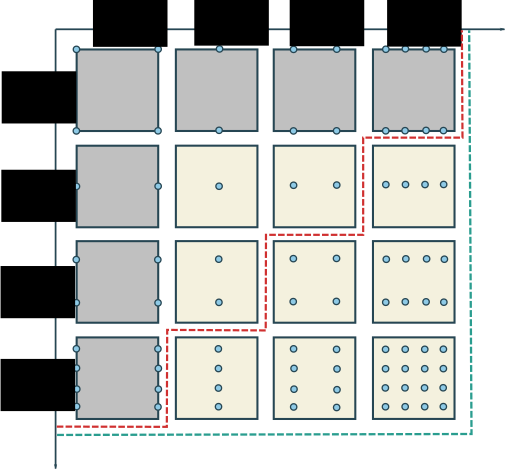
\includegraphics[width=.8\linewidth]{graphics/grid_subspaces}
  \subcaption{Hierarchical splitting of a grid point set}
\label{fig:grid_splitting}
\vspace{2.5mm}
    \end{minipage}%
    \begin{minipage}{0.28\textwidth}
        \centering
  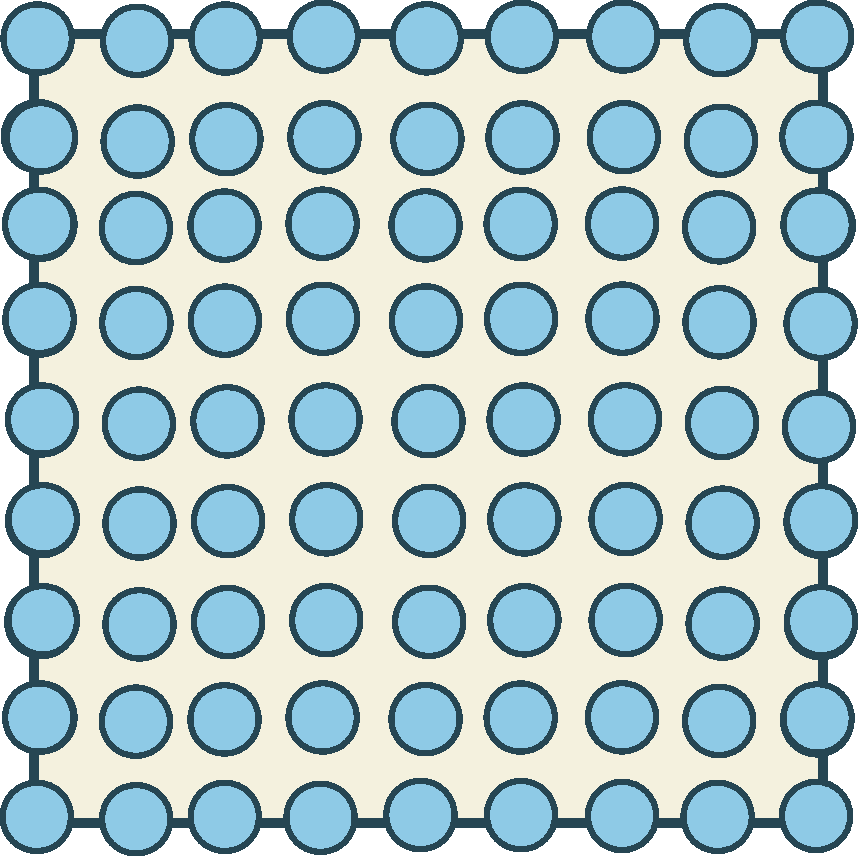
\includegraphics[width=.8\linewidth]{graphics/full_grid}
  \subcaption{Grid points of $V^{\text{fb}}_{3}$}
\label{fig:full_grid}
\vspace{4.5mm}
  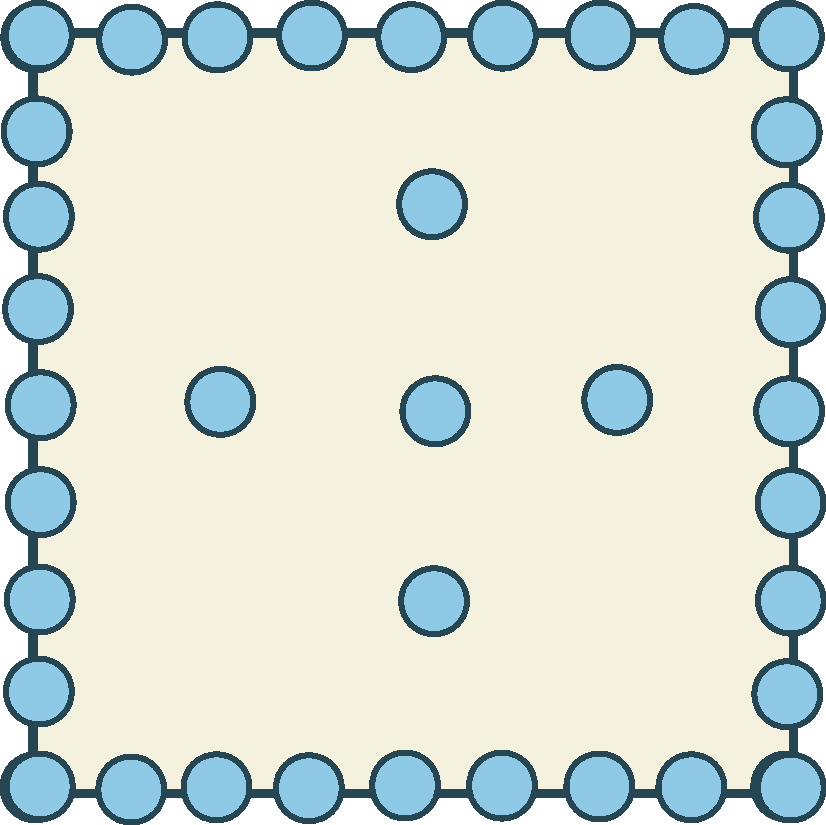
\includegraphics[width=.8\linewidth]{graphics/sparse_grid}
  \subcaption{Grid points of $V^{\text{sb}}_{3}$}
\label{fig:sparse_grid}
\vspace{2.5mm}
    \end{minipage}
\delimit
\caption{Construction of different grids from hierarchical grid point set increments. The full boundary grid $V^{\text{fb}}_{3}$ is a sum of all grid increments outlined in dotted \greencomma\,\,whereas the sparse boundary grid $V^{\text{sb}}_{3}$ is a sum of all grid increments outlined in dotted \reddot\,\,Boundary grid point increments are shaded in \greydot}
\label{fig:grid_construction}
\end{figure}
\end{mdframed}

\section{Basis functions}

Multivariate basis functions $\phi_{\underline{\ell},\underline{i}}$ (\cref{def:basis_functions}), are a central aspect of sparse grids.
Many different families of basis functions exist, each with various levels of complexity, capabilities, and properties.
In this section we will take a short look at the basis functions used in this thesis.

\paragraph{Hat functions}
An elementary basis for sparse grids can be constructed with the help of hat functions, which are just piecewise linear functions.
A one-dimensional hat function, $h(x) \coloneqq \max(1 - |x|,0)$, can be transformed into a basis function for a level $\ell$ and index $i$ to obtain
\begin{equation}
\phi^\mathrm{h}_{\ell,i}(x) \coloneqq h(2^\ell x-i).
\end{equation}
These basis functions are centered at their associated grid point $x_{\ell,i}$.
Furthermore, their supports are disjoint for the same level.
\Cref{fig:basis_hat_normal} shows the hat basis functions for the first few levels.

\paragraph{Modified basis functions}
One method of removing the need of using boundary grid points to accurately approximate some model functions in the boundary regions are modified basis functions \cite{Pflueger2010}.
These basis functions extrapolate the values at the boundaries from the grid points closest to the boundaries by using a modified version of normal basis functions.
Extrapolation of this sort can, at least to some degree, be a viable alternative to using boundary grids as a lot of grid points would be allocated just for the boundaries by high-dimensional sparse grid surrogates.
Removing all of them while still providing acceptable boundary approximations usually results in a good tradeoff between grid points and accuracy, which is the intuition behind sparse grids.
More formally, it is possible to modify any non-boundary basis functions by adding a constant function to it and also defining special boundary extrapolation functions $\phi^{\text{left}}_{\ell}$ and $\phi^{\text{right}}_{\ell}$ that are usually are similar with regards to their construction compared to the normal basis functions $\phi_{\ell,i}$.
For example, modified basis functions for the hat basis can be obtained by adding boundary functions and a constant function to the hat basis with
\begin{equation}
\phi^{\mathrm{mod,h}}_{\ell,i}(x) \coloneqq
\begin{cases}
1,& \ell=1\\
\max(2 - 2^\ell x, 0),& \ell>1, i=1\\
\max(2 - 2^\ell (1 - x), 0),& \ell>1, i=2^\ell - 1\\
\phi^{\mathrm{h}}_{\ell,i}(x),& \text{else}
\end{cases}.
\end{equation}
\Cref{fig:basis_hat_mod} shows the modified hat basis functions for the first few levels.

\begin{mdframed}[style=style]
\begin{figure}[H]
\begin{subfigure}{.5\textwidth}
  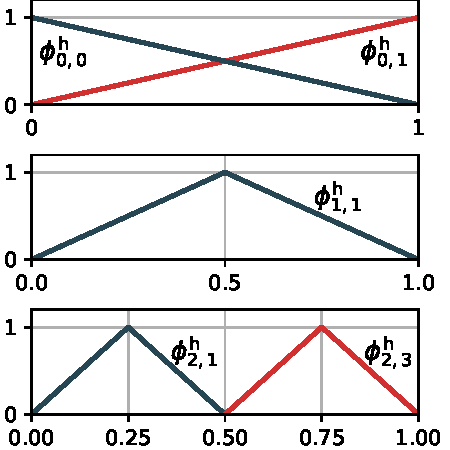
\includegraphics[width=\linewidth]{graphics/basis_hat}
  \subcaption{Hat basis for $\ell=0,\dots,2$.}
  \label{fig:basis_hat_normal}
\vspace{1.5mm}
\end{subfigure}%
\begin{subfigure}{.5\textwidth}
  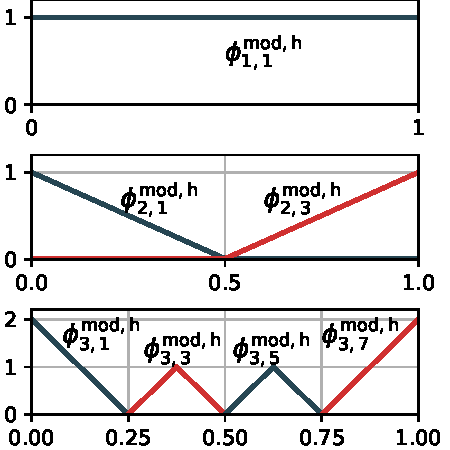
\includegraphics[width=\linewidth]{graphics/basis_mod}
  \subcaption{Modified hat basis for $\ell=1,\dots,3$.}
  \label{fig:basis_hat_mod}
\vspace{1.5mm}
\end{subfigure}
  \delimit
\caption{Hat basis functions and their modified counterparts.}
  \label{fig:basis_hat}
\end{figure}
\end{mdframed}

\paragraph{Other basis functions}
Over time, many kinds of basis functions have been developed.
Each one was created with a specific purpose in mind and has the potential to outshine other basis functions for certain applications.
There exist polynomial basis functions, spline basis functions that are just piecewise polynomials, wavelet basis functions, and numerous subtypes of them.
However, for the sake of simplicity, they are not covered in detail as they will not be primarily used in this thesis.
Instead, we will focus on hat basis functions and modified hat basis functions.

\section{Sparse grid surrogates}
\label{sec:gsc}

Sparse grid surrogates can be constructed using one of multiple different approaches.
As a sparse grid surrogate is a linear combination of all basis functions, in order to represent the instance $\hat{f}$, each basis function $\phi_{\underline{\ell},\underline{i}}$ is assigned a weight $\alpha_{\underline{\ell},\underline{i}}$, also called hierarchical surplus.

\begin{definition}[Sparse grid surrogates]
Let $\phi_{\underline{\ell},\underline{i}}$ be multivariate basis functions and $X$ a set of grid points.
Furthermore, let $\alpha_{\underline{\ell},\underline{i}} \in \mathds{R}$ be the hierarchical surplusses.
A grid surrogate is then a linear combination with
\begin{equation}
\hat{f}(x) \coloneqq \sum_{x_{\underline{\ell},\underline{i}} \in X} \alpha_{\underline{\ell},\underline{i}} ~ \phi_{
\underline{\ell},\underline{i}}(x).
\end{equation}
In the case of a regular sparse grid with $X=X^{\mathrm{s}}_{\ell}$, the surrogate instance can also be expressed with
\begin{equation}
\hat{f}(x) = \sum_{|\underline{\ell}|_1 \leq \ell, \underline{1} \leq \ell'} \sum_{\underline{i} \in {H_{\underline{\ell}}}} \alpha_{\underline{\ell},\underline{i}} ~ \phi_{
\underline{\ell},\underline{i}}(x).
\end{equation}
\end{definition}
%
The hierarchical surplusses can be computed in a variety of different ways, which results in multiple possible sparse grid construction schemes.
Most of the time, the interpolation approach is used.
In cases where only model function observations are given, a sparse grid surrogate can also be constructed through regression

\begin{definition}[Fundamental property]
A family of univariate basis functions $\phi_{\ell,i}$ fulfills the fundamental property iff
\begin{equation}
\begin{split}
&\phi_{\ell,i}(x_{\ell', j}) = 0, ~~  \ell' < \ell, j \in H_{\ell'},\\
&\phi_{\ell,i}(x_{\ell', j}) = \delta_{ij}, ~~  j \in H_{\ell'}.
\end{split}
\end{equation}
As the used multivariate basis functions are constructed using the tensor-product approach, the fundamental property holds for a multivariate basis iff it holds for the univariate one.
\label{def:fund}
\end{definition}

\paragraph{Interpolation}
The interpolation method is the most simple and common sparse grid surrogate construction scheme.
It evaluates the model function at every grid point and performs a hierarchization algorithm to obtain the hierarchical surplusses $\alpha_{\underline{\ell},\underline{i}}$.
A multivariate basis that fulfills the fundamental property can be hierarchized very efficiently through the unidirectional principle \cite{Balder1994} by applying a hierarchization operator iteratively on every dimension separately, effectively breaking down the hierarchization process into a series of one-dimensional hierarchizations.
The resulting surrogate constructed with the hierarchization method equals the model function at all grid points, \ie $\forall x_{\underline{\ell},\underline{i}} \in X \colon f(x_{\underline{\ell},\underline{i}})=\hat{f}(x_{\underline{\ell},\underline{i}})$.
As the model function has to be evaluated at every grid point, a grid interpolation surrogate requires exactly $|X|$ function evaluations and can not be used to approximate a function from only model function observations.

\paragraph{Regression}
An alternative surrogate construction scheme is sparse grid regression \cite{Pflueger2010}.
In contrast to interpolation, a regression approach does no longer require the function values at the grid points to interpolate between them.
Instead, it uses established regression approaches to iteratively improve the weights $\alpha_{\underline{\ell},\underline{i}}$ with regards to the approximation error by using train and validation observations from the model function.
As a result, the amount of required observations does no longer have to be equal to the amount of grid points.
This results in a greater level of flexibility as the amount of available inputs and the amount of grid points can vary.
The basic approach is to solve the least squares problem for the observation set, $S \coloneqq \left\{(x_i, f(x_i)\right\}_{i=1}^n \subseteq \Omega \times \mathds{R}$, with the standard square loss function,
\begin{equation}
\varepsilon_{\text{MSE}}(\hat{f}) \coloneqq \frac{1}{n} \sum_{i=1}^n \left(f(x_i) - \hat{f}(x_i)\right)^2 ,
\end{equation}
which contains a regularization functional $R$ and a regularization control parameter $\lambda > 0$ that allows for smoothing and can also prevent overfitting.
Sparse grid regression therefore tries to solve the regularized least squares problem to find the best possible surrogate for a set of possible regularization factors $\lambda \in \Lambda$ and sparse grid level $\ell$ to obtain the surrogate with
\begin{equation}
\hat{f} = \argmin_{\hat{f} \in V^{\text{s}}_{\ell}, ~ \lambda \in \Lambda} \varepsilon_{\text{MSE}}(\hat{f}) + \lambda R(\hat{f}).
\end{equation}

\section{Spatially adaptive sparse grids}

The process of generating a regular sparse grid can be improved upon in many cases by introducing adaptivity.
This allows us to spend more grid points, and therefore be more accurate, in regions that are more important and conversely reduce the amount of grid points spent in less important regions.
When done correctly, the surrogate can adapt itself to the model function characteristics and deliver a better approximation.
One method of implementing adaptivity during the sparse grid construction process are spatially adaptive sparse grids \cite{Pflueger2012}.
The central idea of them is to define a grid point hierarchy where each non-boundary grid point has two child grid points on the next level increment along every dimension.
A stepwise algorithm then adds these child grid points to the surrogate if they are needed and do not exist yet.
This creation of new grid points that stem from a parent grid point is called the refinement of the parent grid point.

\begin{definition}[Hierarchical grid point children]
Let $X$ be a set of grid points, and let $x_{\underline{\ell},\underline{i}} \in X$ be a grid point.
We define
\begin{equation}
c_{k}^{\mathrm{left}}(x_{\underline{\ell},\underline{i}}) \coloneqq (x_{\ell_1,i_1}, \dots, x_{\ell_k + 1,2  i_k - 1} \dots, x_{\ell_d,i_d})
\end{equation}
as its left child along the $k$-th dimension if $i_k > 0$ and
\begin{equation}
c_{k}^{\mathrm{right}}(x_{\underline{\ell},\underline{i}}) \coloneqq (x_{\ell_1,i_1}, \dots, x_{\ell_k + 1,2  i_k + 1} \dots, x_{\ell_d,i_d})
\end{equation}
as its right child along the $k$-th dimension if $i_k < 2^{\ell_k}$.
In addition, we define
\begin{equation}
c_{k}(x_{\underline{\ell},\underline{i}}) \coloneqq
\begin{cases}
\left\{c_{k}^{\mathrm{right}}(x_{\underline{\ell},\underline{i}})\right\}&, i_k=0\\
\left\{c_{k}^{\mathrm{left}}(x_{\underline{\ell},\underline{i}})\right\}&,i_k= 2^{\ell_k}\\
\left\{c_{k}^{\mathrm{left}}(x_{\underline{\ell},\underline{i}}), ~ c_{k}^{\mathrm{right}}(x_{\underline{\ell},\underline{i}}) \right\}&, \text{else}
\end{cases}
\end{equation}
as the set of children along the $k$-th dimension of the grid point $x_{\underline{\ell},\underline{i}}$, and
\begin{equation}
c(x_{\underline{\ell},\underline{i}}) \coloneqq \bigcup_{k=1}^d \left\{c_{k}(x_{\underline{\ell},\underline{i}})\right\}
\end{equation}
as the set of all children of a grid point.
It always holds that $\abs{c(x_{\underline{\ell},\underline{i}})} \leq 2d$, and in case there is no boundary involved, $\abs{c(x_{\underline{\ell},\underline{i}})}=2d$ holds as well.
Furthermore, we denote a grid point $x_{\underline{\ell},\underline{i}} \in X$ as a leaf if it holds that
\begin{equation}
c(x_{\underline{\ell},\underline{i}}) \cap X = \emptyset,
\end{equation}
\ie no children of it are already contained in $X$.
\end{definition}
%
To choose the best grid points to refine, a refinement criterion is introduced.
This abstract refinement criterion assigns a value to each grid point such that the grid points with the highest values can be refined.
\begin{definition}[Refinement criterion]
Let $X$ be a set of grid points.
We define $\xi \colon X \mapsto \mathds{R}$ as the refinement criterion, which assigns each grid point a value that determines the suitability of a refinement.
The commonly used surplus criterion,
\begin{equation}
\xi_s(x_{\underline{\ell},\underline{i}}) \coloneqq \abs{\alpha_{\underline{\ell},\underline{i}}},
\end{equation}
uses the absolute hierarchical surplus value, as a high value indicates steep rates of change in the area of a grid point.
\end{definition}
%
To prepare for an iterative adaptivity algorithm, we define the grid points of adaptive sparse grids after $m$ steps as $X_a^{(m)}$.
A spatially adaptive sparse grid usually starts out as a regular sparse grid with a coarse level, \ie $X_a^{(0)}=X^{\text{s}}_{\ell}$.
Then, during the $m$-th iteration, we first order all leaf grid points with
\begin{equation}
\xi(x_1) \geq \dots \geq \xi(x_p), ~~ x_1, \dots, x_p \in X_a^{(m-1)},
\end{equation}
and then perform $k$ refinements to obtain $X_a^{(m)}=X_a^{(m-1)} \cup c(x_1) \cup \dots \cup c(x_k)$.
Usually, when a leaf grid point is refined, all children are created because selective children creation would create additional overhead.
After $q$ steps, the spatially adaptive sparse grid is finished and consists out of the grid points $X_a^{(q)}$.
Important parameters that influence the results are the amount of iterations $q$, the refinements per step $k$, the refinement criterion $\xi$, as well as the initial grid type and size of $X_a^{(0)}$.

There also exist various other established adaptivity methods that adapt the underlying grid in other ways.
For example, dimensionally adaptive sparse grids use a more rigid refinement rule that adds the grid points of whole hierarchical subspaces to the surrogate.
One small downside of spatially adaptive sparse grids is that usually all child grid points are added in a refinement step.
In a dimensionality reduction focused setting this behaviour is not optimal, since we want to focus on more important dimensions when refining a grid point.
One more recently introduced method are spatially dimension adaptive sparse grids \cite{Khakhutskyy2016} that provide a solution for this by only selectively adding child grid points along certain dimensions.

\section{Radial basis functions}
\label{sec:rbf}

Radial basis function surrogates \cite{Broomhead1988} are another way of approximating a model function by utilizing radial basis functions.
A radial basis function $\varphi' \colon \Omega \mapsto \mathds{R}$ is a function whose value solely depends on the distance between the input and its associated center point $c \in \Omega$.
More formally, there must exist a function $\varphi$ such that $\varphi'(x)=\varphi(\|x - c\|)$ holds.
Functions that fulfill this property are called radial functions and the associated univariate function $\varphi$ is called a radial kernel centered at $c$.
Similar to sparse grid surrogates, a radial basis function surrogate is a linear combination of $m$ radial basis functions with center points $c_i$ and weights $\omega_i$ with
\begin{equation}
f(x) \approx \sum_{i=1}^m \omega_i \varphi(\|x - c_i\|).
\end{equation}
In the context of this thesis, only Gaussian functions with the Euclidean distance ${|\cdot |}_2$ measure,
\begin{equation}
\varphi(x) \coloneqq e^{-(\epsilon \abs{x - c_i}_2)^2},
\end{equation}
are used as basis functions.
The only parameter that can be tuned is $\epsilon$, which is referred to as the shape parameter and is used to scale the effects of the input radius.
Given a set of center points, type of basis functions, and shape parameter $\epsilon$, we can calculate the weight coefficients $\omega_i$ by solving a linear least squares problem.
This, combined with the fact that exponentially more center points are needed to maintain the same level of coverage when the model dimensionality increases, also causes this method to suffer from the curse of dimensionality.

Radial basis function approximation is covered in this thesis as it is almost a polar opposite to grid-based approximation.
Sparse grid surrogates require a hierarchical and axis-aligned grid, while radial basis function surrogates allow us to specify arbitrary center points.
Furthermore, radial basis functions are fundamentally different to tensor-product-based basis functions with regards to their orientation.
While tensor product basis functions are strictly axis-aligned, radial basis functions are unaware of the concept of axis-alignment or orientation as only the radius matters to them.
This property will allow us to use radial basis functions as a reference when investigating the effects of basis function alignment later on.

\section{Sampling}
\label{sec:lds}

In the coming chapters we will make use of regression and some Monte-Carlo-based methods, both of which requiring model function observations as inputs.
For this purpose, even the relatively simple process of drawing samples from the input parameter probability distribution of the model can improved to achieve better results.
We assume that the inputs of model functions are distributed according to a $d$-dimensional multivariate distribution defined by the probability density function,
\begin{equation}
\rho(x) \coloneqq \prod_{i=1}^d \rho_i(x_i),
\end{equation}
which is made up out of $d$ independent distributions $\rho_i$.

A problem that arises when using a pseudorandom number generator to draw samples from the $d$-dimensional uniform input distribution is that the sequence does not cover the function domain as evenly and quickly as it theoretically can.
One solution are so-called low-discrepancy sequences, which are also called quasirandom sequences to distinguish them from normal pseudorandom sequences.
These sequences are more evenly distributed than pseudorandom samples and therefore have a lower discrepancy.
Thus, they cause the result of various Monte-Carlo methods to converge faster than it would if we were just using the same amount of pseudorandom samples.
A commonly used quasirandom sequence is the Sobol sequence \cite{Niederreiter1988}, which is also used in this thesis.
It is generated using the Antonov and Saleev variant that uses the Gray code of $i$ to construct the $i$-th sample.

This approach can also be extended to allow for the generation of pseudorandom samples from non-uniform distributions through the commonly used inverse transform sampling method \cite{Devroye1986}.
However, this approach is not used in this thesis as the gains are minimal.

\section{Error metrics}
\label{sec:errors}

To evaluate the quality of a constructed surrogate $\hat{f}$, we define a couple of error metrics to measure the approximation error and also make it comparable to other surrogates.
An established and commonly used error metric in the context of sparse grids is the $L^2$ error:
\begin{definition}[$L^2$ error]
Let
\begin{equation}
{\|g\|}_{L^p}^p \coloneqq \int_{\Omega} \abs{g(x)}^p \mathrm{d}x
\end{equation}
be the $L^p$ norm for a real function $g \colon \Omega \mapsto \mathds{R}$.
We then define
\begin{equation}
\varepsilon_{\text{$L^2$}}(f, \hat{f}) \coloneqq \|f - \hat{f}\|_{L^2}=\sqrt{\int_{\Omega} {\abs{f(x) - \hat{f}(x)}}^2 ~ \mathrm{d}x}
\end{equation}
as the $L^2$ surrogate approximation error.
\label{def:l2}
\end{definition}
%
In numerics, to evaluate the accuracy of an estimator, the mean squared error and the root mean squared error are commonly used.
These metrics can be described as the expected value of the squared errors and its square root, respectively.

\begin{definition}[Mean squared errors]
Let $\hat{f}$ be model function surrogate for $f$ and $S=\left\{(x_i, f(x_i)\right\}_{i=1}^n \subseteq \Omega \times \mathds{R}$ a set of observations.
We define
\begin{equation}
\varepsilon_{\mathrm{MSE}}(f, \hat{f}) \coloneqq \frac{1}{n} \sum_{i=1}^n \left(f(x_i) - \hat{f}(x_i)\right)^2
\end{equation}
as the mean squared approximation error of the surrogate.
In the same fashion, we also define
\begin{equation}
\varepsilon_{\mathrm{RMSE}}(f, \hat{f}) \coloneqq \sqrt{\varepsilon_{\mathrm{MSE}}(f, \hat{f})} = \sqrt{\frac{1}{n} \sum_{i=1}^n \left(f(x_i) - \hat{f}(x_i)\right)^2}
\end{equation}
as the root mean squared error of the surrogate.
\end{definition}
%
The RMSE is closely related to the continuous $L^2$ error as it is just a discrete version of it in case the observations $S$ are uniformly distributed.
Thus, it holds that
\begin{equation}
\lim_{n \to \infty} \varepsilon_{\mathrm{RMSE}}(f, \hat{f}) = \varepsilon_{\text{$L^2$}}(f, \hat{f})
\end{equation}
when the inputs are uniformly distributed.

One problem of these error metrics is that they are all sensitive to the magnitude of the function values.
To improve upon these absolute error metrics and allow for comparisons across model functions with different ranges of function values, we define normalized error metrics.

\begin{definition}[Normalized root mean squared error]
Let $\hat{f}$ be a model function surrogate for $f$ and $S=\{(x_i, f(x_i)\}_{i=1}^n \subseteq \Omega \times \mathds{R}$ a set of observations.
We define
\begin{equation}
\varepsilon_{\mathrm{NRMSE}}(f, \hat{f}) \coloneqq \frac{\varepsilon_{\mathrm{RMSE}}(f, \hat{f})}{\max\limits_{(x, f(x)) \in S} f(x) - \min\limits_{(x, f(x)) \in S} f(x)}
\end{equation}
as the normalized root mean squared error.
\end{definition}


\chapter{Input transformations}
\label{chap:c3}

A lot of work has already gone into exploring all kinds of variants and optimizations for sparse grids that resulted in many different families of basis functions and grid types, showcased for example in \cite{Feuersaenger2010, Valentin2019}.
Moreover, many methods and algorithms that work on sparse grids have also been developed, for example in \cite{Gerstner1998, Garcke2001, Pflueger2010, Valentin2019, Rehme2021}, and allow the general sparse grids technique to be applied in a better and more flexible way to many different kinds of problems.
In the related literature, optimizing the sparse grid construction process itself was the primary focus most of the time.
In contrast to this approach, we instead inspect and adapt the inputs itself prior to constructing any sparse grid.
The basic idea that is propagated in this thesis is that, instead of directly using the sparse grids to approximate a function with $f(x) \approx \hat{f}(x)$, we insert another layer of flexibility into the process by introducing an input transformation function $t$ and creating a surrogate $\hat{f}_t$ in tandem with $t$ such that a transformed sparse grid approximation $f(x) \approx \hat{f}(t(x))$ performs better.
This general idea and also the necessary details will be expanded upon in this chapter.

\section{Intrinsic dimensionality}
\label{sec:intrinsic}

There already exist several techniques used in signal processing and data science that are related to the idea of input transformations, for example principal component analysis (PCA) \cite{Abdi2010}, which tries to find and exploit certain characteristics of the input data.
Related to PCA is the concept is intrinsic dimensionality \cite{Bennett1969}.
The intrinsic dimensionality of a function or dataset is the minimal amount of features required to completely represent its output.
It can be used as a guidance to determine the actual dimensionality of the model function and also optionally exploit the knowledge to construct a lower-dimensional surrogate, \ie performing a dimensionality reduction.

\begin{definition}[Intrinsic dimensionality]
A $d$-dimensional modelfunction $f \colon \Omega \mapsto \mathds{R}$ has an intrinsic dimensionality of $r \leq d$ if there exists an $r$-dimensional function $f_t \colon \Omega_r \mapsto \mathds{R}$ and a transformation function $t \colon \Omega \mapsto \Omega_r$ such that
\begin{equation}
\forall x \in \Omega \colon f(x)=f_t(t(x)).
\end{equation}
\label{def:intrinsic}
Even though we do not explicitly define $\Omega_r$, it should also be a bounded Euclidean product such that it can  transformed into the unit hypercube $\Omega_r=[0,1]^r$.
\end{definition}
%
We denote the minimal intrinsic dimensionality of a function as $r^\ast$.
Even if we are able to find a non-optimal $r$-dimensional transformation with $r > r^\ast$ that satisfies the requirement of \cref{def:intrinsic}, we still have gained an advantage and can define that function as having an intrinsic dimensionality of at most $r$.
Furthermore, in case it holds that $r=r^\ast$, we still refer to it as having an intrinsic dimensionality of at most $r$ because the true minimal intrinsic dimensionality $r^\ast$ is often unknown.

Since we are dealing with function approximation problems in this thesis, we extend \cref{def:intrinsic} to also allow for approximation errors:
\begin{definition}[Approximate intrinsic dimensionality]
Let $f$ be a $d$-dimensional function, and $\varepsilon$ an error metric.
We then define $f$ as having an approximate intrinsic dimensionality of $r \leq d$ with an error of $e$, if there exists an $r$-dimensional function $f_t \colon \Omega_r \mapsto \mathds{R}$ and a function $t \colon \Omega \mapsto \Omega_r$ such that
\begin{equation}
e=\varepsilon\left(f,  f_t \circ t\right).
\end{equation}
\end{definition}
%
Similar to the minimal intrinsic dimensionality $r^\ast$, we are not concerned about the finding, and also usually do not know, the minimal error $e^\ast=\min_{t, f_t} \varepsilon\left(f,  f_t \circ t\right)$ for a given $r$.
The introduction of approximation errors also enables us to determine a good tradeoff between intrinsic dimensionality and approximation error.

To achieve a good convergence rate and general representativeness when performing an operation on the model function that makes use of observations, \eg a Monte-Carlo quadrature operation, it is important to achieve a low discrepancy and thus cover the input space $\Omega$ more evenly.
Under normal circumstances, to achieve the same discrepancy in a high-dimensional space as in a low-dimensional space,
exponentially more observations are required.
However, combining this requirement with the concept of intrinsic dimensionality, we observe that we effectively only need to cover $\Omega_r$ and adapt any operation that normally works on $f$ to instead work on the lower dimensional function $f_t$.
Therefore, the amount of observations required to achieve a good coverage of the domain of $f_t$ would depend on $r$ and not on $d$.

\begin{definition}[Transformed distribution]
Let $t^{-1}(x_{t})=\{x \in \Omega \mid t(x)=x_{t}\}$ be the inverse transformation function.
We then define the transformed distribution,
\begin{equation}
\rho_t \colon \Omega_r \to \mathds{R_+}, ~~ \rho_t(x_t)=\int_{t^{-1}(x_t)} \rho(x) \; \mathrm{d}x.
\end{equation}
This is also a valid probability distribution since
\begin{equation}
\int_{\Omega_r} \rho_t(x_t) \; \mathrm{d}x_t=\int_{\Omega_r} \int_{t^{-1}(x_t)} \rho(x) \; \mathrm{d}x_t = \int_{\Omega} \rho(x) \; \mathrm{d}x = 1
\end{equation}
and $\rho_t(x_t) \geq 0$ holds.
\end{definition}
%
One thing to take note of is that applying a transformation on the original input distribution $\rho$ has the potential to change the distribution type.
For example, in case of a uniform distribution $\rho=\mathcal{U}[0,1]^d$, the associated transformed distribution $\rho_t$ could be a non-uniform distribution.
To effectively sample from $\rho_t$, it is still easier to just draw the samples $(x_1, \dots, x_n)$ from $\rho$ directly and feed them into the transformation function to obtain the transformed sequence $(t(x_1), \dots, t(x_n))$, which is distributed according to $\rho_t$.
The general quality and properties of transformed low discrepancy sequences (\cref{sec:lds}) also change compared to its original, untransformed sequence \cite{Wang2008}.

\section{Limitations of sparse grids}

All grid-based interpolation methods share the common problem of being affected by the curse of dimensionality \cite{Bellman1961}, which effectively puts an upper limit on the feasible dimensionality of sparse grid surrogates.
Sparse grids itself are already a pretty effective strategy to reduce the consequences of the curse of dimensionality compared to full grids because they provide a good tradeoff between the amount of grid points used and their approximation quality.
However, sparse grids can only weaken the curse of dimensionality and delay the effects of it a bit more.
Therefore, employing some form of dimensionality reduction is necessary for high-dimensional models.
Of course, the feasability and effectiveness of dimensionality reduction techniques is limited by the minimum amount of accuracy that is required for the specific use case.
In this section, we take a look at a few already established approaches to dimensionality reduction in the context of sparse grids and take a look at their properties with the help of simple example functions.

The first example function,
\begin{equation}
f_1(x_1, x_2)=\sin(2 \pi x_1) + 1,
\end{equation}
is designed to be a good fit for grid-based methods.
It is a two-dimensional function, where only the first component and a constant term contribute to the total function value, while the second component is unused.
We can easily see that it has an intrinsic dimensionality of $1$ according to \cref{def:intrinsic} since a transformation function could just cut off the second input component.
By simply rotating the function by a few degrees, we obtain the second example function,
\begin{equation}
f_2(x_1,x_2)=\sin(2 \pi x_1') + 1, ~~~~~ x_1'=\cos(0.15 \pi) x_1 -\sin(0.15 \pi) x_2,
\end{equation}
which is also a two-dimensional function but more importantly still has an intrinsic dimensionality of $1$.

\subsection{Spatially adaptive sparse grids}

We start off by interpolating both functions using spatially adaptive sparse grids to investigate how their generated grid points and interpolation errors compare.

\begin{mdframed}[style=style]
\begin{figure}[H]
\begin{subfigure}{.5\textwidth}
  \centering
  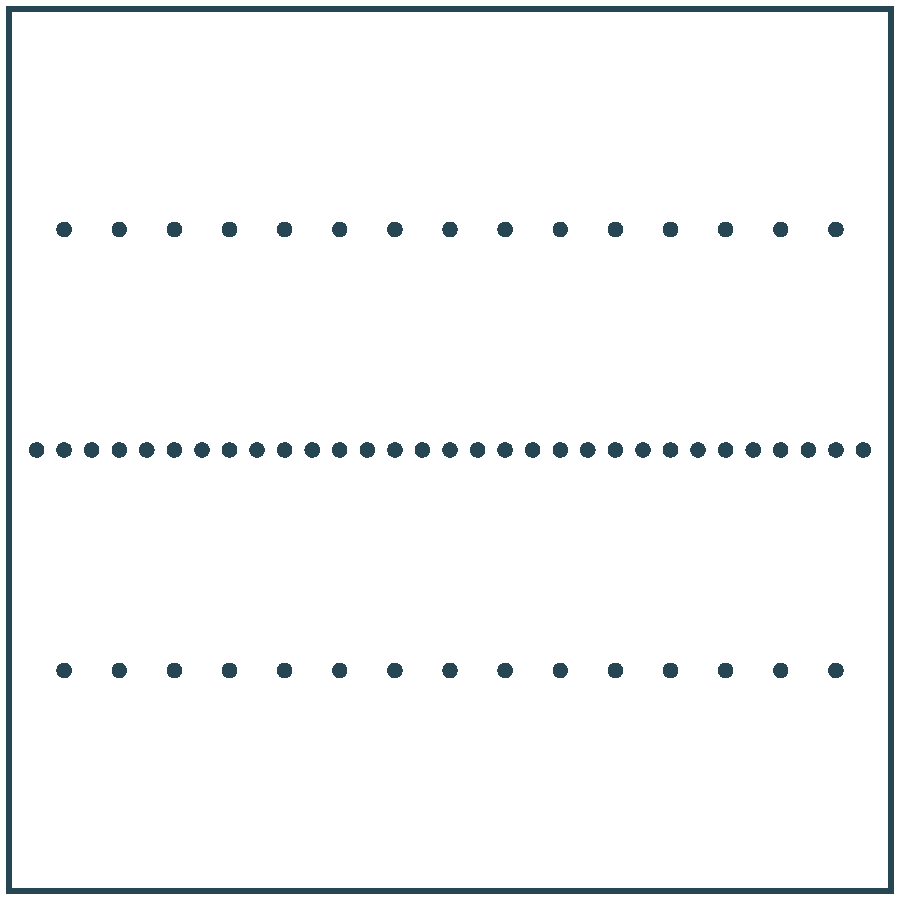
\includegraphics[width=.65\linewidth]{graphics/grid_f1}
  \subcaption{Surrogate grid points for $f_1$}
  \label{fig:grid_f1}
\vspace{2.5mm}
\end{subfigure}%
\begin{subfigure}{.5\textwidth}
  \centering
  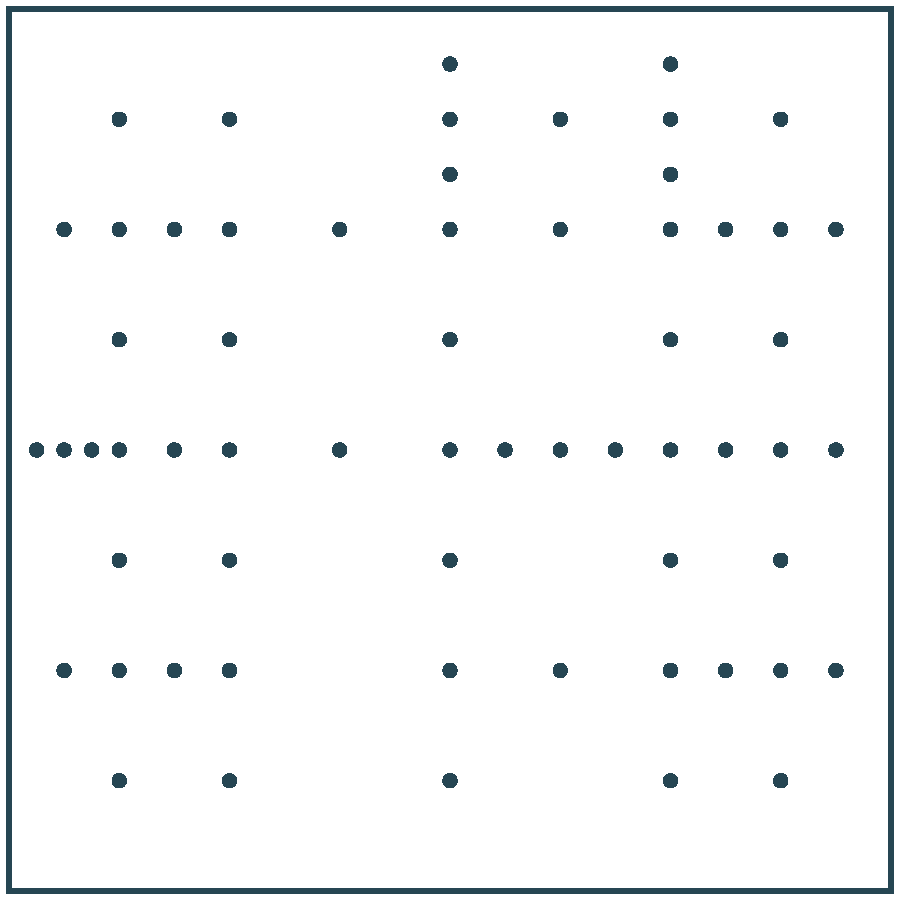
\includegraphics[width=.65\linewidth]{graphics/grid_f2}
  \subcaption{Surrogate grid points for $f_2$}
  \label{fig:grid_f2}
\vspace{2.5mm}
\end{subfigure}
\delimit
\caption{Grid points of generated spatially adaptive sparse grids for $f_1$ and $f_2$.
The sparse grids uses modified hat basis functions and started out as a regular sparse grid with level $\ell=1$. Moreover, the surplus refinement criterion and 15 refinements steps with one grid point refinement per step were used to adapt the sparse grids.}
\label{fig:grids}
\end{figure}
\end{mdframed}
%
\Cref{fig:grids} illustrates how spatially adaptive sparse grids are affected by the different alignment of the input functions.

The spatially adaptive strategy is able to exploit the one-dimensional nature of $f_1$ in \cref{fig:grid_f1} by only refining along the first dimension and therefore spending the grid points only where they matter.
Note that due to the default refinement rule that add all child grid points, the upper and lower grid point rows are created even though they are not necessary.
A tweaked refinement rule could easily fix this.

However, as we can see, \cref{fig:grid_f2}, the intrinsically one dimensional function $f_2$ can not be exploited as it is no longer axis-aligned.
This can be deduced from the fact that grid points all over the grid and along both dimensions are refined.
Moreover, this observation is reinforced by the actual approximation errors of surrogates for both functions seen in \cref{fig:grid_approx_f2}.

\subsection{Radial basis functions}

Radial basis functions behave differently than sparse grids when being applied to the same two functions as their basis functions are not constructed using the tensor-product approach.
Instead, they are orientation agnostic because only the radius relative to a support point determines the basis function value.
Therefore, as seen in \cref{fig:grid_approx_f1}, the approximation errors stay pretty much identical in both cases.
However, the general approximation quality for $f_1$ is worse compared to the sparse grid approximation since radial basis functions are not well suited for approximating functions that are constant along a dimension.
Modified basis functions come with a special constant basis function that is well suited for this purpose and therefore have an advantage.

\begin{mdframed}[style=style]
\begin{figure}[H]
\begin{subfigure}{.5\textwidth}
  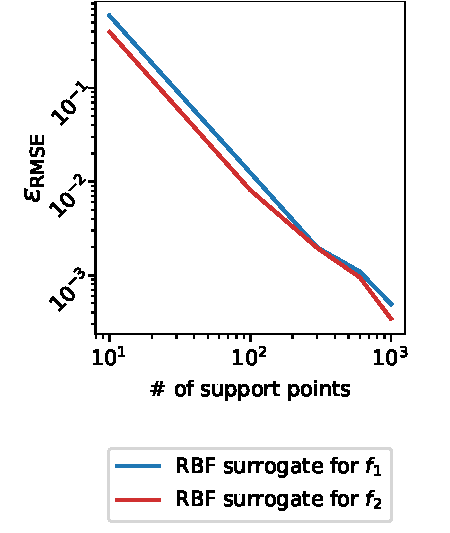
\includegraphics[width=\linewidth]{graphics/grid_approx_f1}
  \subcaption{RBF surrogates created with Gaussian basis functions, Euclidean distance measure, and shape parameter $\epsilon=0.5$.}
  \label{fig:grid_approx_f1}
\vspace{2.5mm}
\end{subfigure}%
\begin{subfigure}{.5\textwidth}
  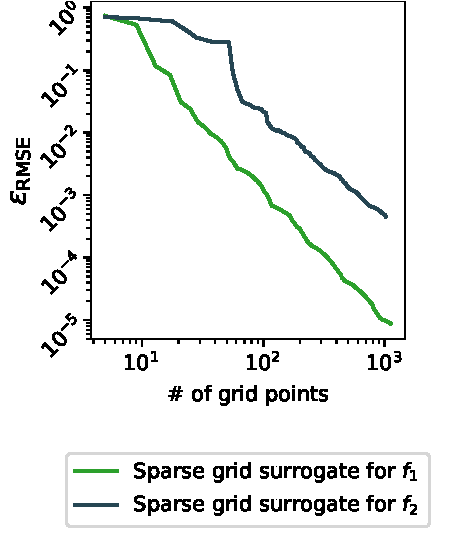
\includegraphics[width=\linewidth]{graphics/grid_approx_f2}
  \subcaption{Spatially adaptive sparse grids with $\ell=1$, surplus refinement criterion, 280 single refinement steps, and mod. hat basis functions.}
  \label{fig:grid_approx_f2}
\vspace{2.5mm}
\end{subfigure}
  \delimit
\caption{
Approximation error comparison between radial basis functions and spatially adaptive sparse grids for both example functions $f_1$ and $f_2$.}
  \label{fig:dim_reduction_errors}
\end{figure}
\end{mdframed}

\subsection{Variance-based sensitivity analysis}

The method of variance-based sensitivity analysis, a form of global sensitivity analysis introduced by Sobol \cite{S01}, is a well established method in statistics to determine the importance of model input parameters.
Given a set of dimension indices $D=\{1,\dots,d\}$, we define the set of ANOVA components with $C \coloneqq \mathcal{P}(D)$ where an ANOVA component $c \in C$ that contains a specific dimension index $i \in D$ indicates that a function term is varying along the $i$-th dimension.
We can then decompose a model function into a componentwise sum with
\begin{equation}
f(x)=\sum_{c \in \mathcal{P}(D)} f_{c}(x),
\label{anovaComp}
\end{equation}
which is called the ANOVA decomposition of $f$.

A decomposition of a high-dimensional function into $|\mathcal{P}(D)|=2^d$ lower-dimensional function terms allows for an examination of individual terms with the goal of identifying terms that contribute the least amount of variance to the total function variance.
This decomposition can also be employed on sparse grids \cite{Feuersaenger2010} by using special semi-orthogonal basis functions, for example pre-wavelet basis functions, to represent the terms $f_c$.
The terms $f_i$ are required to be semi-orthogonal such that can define the variance function,
\begin{equation}
\sigma^2(f) \coloneqq \int_{\Omega} f(x)^2 \rho(x) ~ \text{d} x=\sum_{c \in \mathcal{P}(D)} \sigma^2(f_c),
\end{equation}
in an additive manner.
For every ANOVA component $c \in C$, we are then able calculate the variance share, also called Sobol index,
\begin{equation}
S_{c} \coloneqq \frac{\sigma^2(f_{\underline{c}} )}{\sigma^2(f)}, ~~ \sum_{c \in \mathcal{P}(D)} S_{c} = 1.
\end{equation}
Computing the Sobol indices of all terms for both example functions gives insight into the structure of the function and tells us what share of the function we are able to represent with axis-aligned terms of varying dimension.
It also helps us to understand why spatial adaptivity only works well for one of them.
The Sobol method decomposes the two-dimensional functions into four axis-aligned terms.
A constant term $f_\emptyset$, two one-dimensional terms $f_{\{1\}}$ and $f_{\{2\}}$, and a two dimensional term $f_{\{1,2\}}$.

\begin{mdframed}[style=style]
\begin{figure}[H]
        \centering
\begin{minipage}[H]{.45\textwidth}
  \centering
  \begin{tabular}{ l | c c }
& $2 \notin c~$ & $2 \in c$ \\
\hline
$1 \notin c$ & 0.667 & 0.0\\
$1 \in c$ & 0.333 & 0.0\\
\end{tabular}
\delimit
  \captionof{table}{Sobol indices for all ANOVA components of $f_1$.}
  \label{tab:anova_f1}
    \end{minipage}%
    \hspace{.05\textwidth}
    \begin{minipage}[H]{0.45\textwidth}
  \centering
  \begin{tabular}{ l | c c }
& $2 \notin c~$ & $2 \in c$ \\
\hline
$1 \notin c$ & 0.636 & 0.001\\
$1 \in c$ & 0.163 & 0.199\\
\end{tabular}
\delimit
  \captionof{table}{Sobol indices for all ANOVA components of $f_2$.}
  \label{tab:anova_f2}
    \end{minipage}
\end{figure}
\end{mdframed}
%
As we can see in \cref{tab:anova_f1}, the method correctly identifies that only the terms $f_\emptyset$ and $f_{\{1\}}$ have some output variance with $\sigma^2(f_\emptyset)=0.667 > 0$ and $\sigma^2(f_{\{1\}})=0.333 > 0$.
Therefore, the other terms can be dropped and the function can be completely represented using only one-dimensional function terms.

However, we can see in \cref{tab:anova_f2} that the Sobol method attributes a share of output variance to all terms, since  it holds that $\sigma^2(f_{c}) > 0$ for all ANOVA components.
In this case, the Sobol method shows us that no dimensionality reduction can be performed, as the two-dimensional term $f_{\{1,2\}}$ has a decent amount of variance contribution.
Note that if the constant term $f_\emptyset$ is excluded from the analysis, as is often done, the effects of the changed alignment of $f_2$ on the Sobol indices would be even greater.

\subsection{Summary}

To summarise, we saw that a fundamental property of any approximation method that uses basis functions created using the tensor-product approach is that the approximation quality significantly depends on whether the model function primarily also consists out of axis-aligned terms or not.
In contrast to this behaviour, other basis functions, \eg radial basis functions, do not depend on the alignment of the function terms they are trying to approximate, \ie they can be seen as orientation agnostic.
In turn this means that an effective dimensionality reduction with conventional sparse grid based methods is highly dependent on the alignment of the model function.

Without adding another layer of flexibility, sparse grids can not use their full potential in many cases as we have seen with the function $f_2$.
If we were somehow able to change the alignment of a model function in a more axis-aligned way that matches the underlying sparse grid surrogate, we could improve the approximation in general and also allow a more efficient dimensionality reduction to take place.
In other words, the goal is to transform problems that, due to their alignment, produce results such as \cref{tab:anova_f2} into problems that are more suitable for sparse grids as in \cref{tab:anova_f1}.
This will allow us to perform a better dimensionality reduction.

\section{Active direction transformations}

The concept of intrinsic dimensionality allows us, at least in theory, to use arbitrary transformation functions to map into the lower-dimensional input space $\Omega_r$.
For this purpose, there are numerous possible types of transformation functions to choose from.
As an example, the previous chapter showed how a simple change of basis of the input parameters can have a huge impact on constructed sparse grid surrogates.
We will therefore start out with constructing an orthonormal transformation matrix $W \in \mathds{R}^{d \times d}$ to transform the inputs into a new coordinate system prior to passing them to a sparse grid surrogate.
A good first choice of new basis vectors would be some form of directions along which the model function output has high rates of change.
Various data analysis methods, such as PCA \cite{Abdi2010} or active subspaces \cite{Constantine2015}, employ some form of a singular value decomposition to obtain these directions of high change.
As the active subspace method will be used later on to obtain $W$, we will refer to the new basis vectors of the matrix $W$ as active directions, which is consistent with the active subspace method.
We then refer to the matrix $W$ as the active direction matrix and assume that its basis vectors are ordered by the level of change from highest to lowest, \ie it should hold that the column vector $w_1$ is the most active direction while $w_d$ is the most inactive direction.

After performing a change of basis with $W$ on the inputs, we can effectively eliminate the most inactive dimensions, as all active directions are now mapped onto dimensions in the new coordinate system.
This results in the possibility of drastically reducing the surrogate dimensionality while only suffering a small increase in the approximation error, as only the most inactive directions, which should not contribute a lot to the model function, are eliminated that way.

\begin{definition}[Reduced active direction matrix]
Let $W \in \mathds{R}^{d \times d}$ be an active direction matrix with $W^T W=I$, and let $r \leq d$ be the reduced dimensionality.
We then define
\begin{equation}
W_r \coloneqq \begin{bmatrix}
  \\
    w_1 ~ w_2 ~ \dots ~ w_{r-1} ~ w_r\\
    \\
  \end{bmatrix}
\end{equation}
as the reduced active direction matrix.
\end{definition}
%
As we can see, the reduced active direction matrix is simply obtained from a given active direction matrix $W$ and a reduced dimension $r$ by cutting off the last $d - r$ directions from $W$.
For now, we assume that $W$ and $r$ are given as we will cover the process of determining those essential inputs later on in detail.

\subsection{Unit hypercube projections}

To construct a transformation function $t$ that maps from the $d$-dimensional unit hypercube $\Omega=[0,1]^d$ to the $r$-dimensional unit hypercube $\Omega_r=[0,1]^r$ with $r < d$ for a given transformation matrix $W_r$, several adjustments have to be made in order to obtain a usable transformation function as the naive linear transformation approach with $W_r^T x$ would map inputs outside of $\Omega_r$ in some cases.
When applying a transformation $W_r^T x$ on the elements of a hypercube $x \in \Omega$, the result can be described with the help of zonotopes.

\begin{definition}[Zonotope]
Let $m$ be the dimensionality of the zonotope, and let $k \geq m$ be the amount of zonotope generators.
We define the set
\begin{equation}
Z \coloneqq \left\{\sum_{i=1}^k g_i x_i \mid ~ -1 \leq x_i \leq 1\right\}
  \label{zonotope}
\end{equation}
as an $m$-dimensional zonotope with $k$ generator vectors $g_1, \dots g_k \in \mathds{R}^m$.
\end{definition}

\begin{mdframed}[style=style]
        \centering
\begin{minipage}{.4\textwidth}
        \centering
  \captionof{figure}{Exemplary zonotope with $m=2$, $k=3$, and the three generators $g_1$, $g_2$, $g_3$.
  The outline of the zonotope is coloured in \darkblue and the origin in \reddot}
  \label{fig:zonotope}
    \end{minipage}%
    \begin{minipage}{0.6\textwidth}
        \centering
        \vspace{3.5mm}
  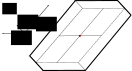
\includegraphics[width=0.8\linewidth]{graphics/zonotope}
  \hspace{-5.5mm}
    \end{minipage}
\end{mdframed}
%
When applying the projection $W_r^T$ to the inputs $x \in \Omega$, we can observe that
\begin{equation}
\begin{split}
W_r^T x=~W_r^T \sum_{i=1}^d x_i e_i=~\sum_{i=1}^d x_i w_i , ~~~~ w_i=W_r^T e_i,
\end{split}
\end{equation}
where the $w_i$ are just the transformed unit vectors.
Therefore, since for all components are contained in the unit interval with $x_i \in [0,1]$, we can express the transformed inputs with
\begin{equation}
\{W_r^T x \mid x \in \Omega\}=\left\{\sum_{i=1}^d x_i w_i \mid x \in \Omega \right\}=\left\{ \sum_{i=1}^r x_i w_i \mid 0 \leq x_i \leq 1\right\}.
\label{wtx}
\end{equation}
To get \cref{wtx} closer to the zonotope definition \cref{zonotope}, we first center the inputs $x \in \Omega$ before applying the transformation and divide the vectors $w_i$ by 2.
For this, we define $c_i=\underline{0.5}$ as the center of the $i$-dimensional unit hypercube.
We observe that a linear transformation using $W_r$ on centered inputs will yield the following result:
\begin{equation}
\begin{alignedat}{2}
&\left\{W_r^T (x - c_d) \mid x \in \Omega\right\}&&=\left\{W_r^T \sum_{i=1}^d \left(x_i - \frac{1}{2}\right) e_i \mid x \in \Omega \right\}\\
=&\left\{\sum_{i=1}^d \left(x_i - \frac{1}{2}\right) W_r^T e_i \mid x \in \Omega \right\}&&=\left\{\sum_{i=1}^d \left(x_i - \frac{1}{2}\right) w_i \mid x \in \Omega \right\}, ~~ w_i=W_r^T e_i\\
=&\left\{\sum_{i=1}^d \left(x_i - \frac{1}{2}\right) w_i \mid 0 \leq x_i \leq 1 \right\}&&=\left\{\sum_{i=1}^d x_i w_i \mid -\frac{1}{2} \leq x_i \leq \frac{1}{2} \right\}\\
=&\left\{\sum_{i=1}^d \frac{1}{2} x_i w_i \mid -1 \leq x_i \leq 1 \right\}&&=\left\{\sum_{i=1}^d x_i p_i \mid -1 \leq x_i \leq 1 \right\}, ~~ p_i=\frac{1}{2} w_i
\label{zonotope_form}
\end{alignedat}
\end{equation}
%
Therefore, the codomain of a centered transformation with $W_r$ is equal to the zonotope
\begin{equation}
Z_{p} \coloneqq \left\{\sum_{i=1}^d x_i p_i , ~ -1 \leq x_i \leq 1\right\}, ~~ p_i \coloneqq \frac{1}{2} W_r^T e_i,
\end{equation}
and the image of the function
\begin{equation}
p \colon \Omega \mapsto Z_p, ~~ p(x)=W_r^T (x-c_d)
\end{equation}
is equal to $Z_p$, \ie it holds that $Z_{p}=p(\Omega)$.

\subsection{Surrogate space}

After we obtained a zonotope $Z_p$, the next step is to determine how to go from this zonotope to a hypercube because sparse grid surrogates require the domain to be the unit hypercube.
To achieve this, the zonotope $Z_p$ is first encased in an $r$-dimensional hypercube, called the surrogate space $S$, which is then scaled and aligned to obtain the unit hypercube $\Omega_r$.
The generators $q_1, \dots, q_r$ of the encasing hypercube can be calculated by applying the Gram–Schmidt process on the ordered zonotope generators $p_i$ to obtain the orthogonal vectors,
\begin{equation}
q_i \coloneqq \frac{q_i'}{\| q_i' \|},~~ q_i' \coloneqq p_i - \sum_{k=1}^{i-1} \frac{\langle p_k, q_k'\rangle}{\langle q_k', q_k' \rangle} q_k'.
\label{q}
\end{equation}
%
The surrogate space, which encases the zonotope $Z_p$, is then an $r$-dimensional hypercube,
\begin{equation}
S \coloneqq \left\{\sum_{i=1}^r s_i q_i x_i, ~ -1 \leq x_i \leq 1\right\},~~ s_i \coloneqq \sum_{k=1}^d \langle q_i, p_k\rangle,
\label{surrogate_space}
\end{equation}
where the scaling factors $s_i$ are chosen in such a way that the hypercube $S$ exactly matches the extent of the zonotope $Z_p$, as seen in \cref{fig:surrogate_space}.

\begin{mdframed}[style=style]
        \centering
\begin{minipage}{.49\textwidth}
        \centering
  \captionof{figure}{Construction of the encasing surrogate space $S$ according to \cref{surrogate_space} for the zonotope $Z_p$ from \cref{fig:zonotope}.
  The outline of the zonotope $Z_p$ is coloured in \lightbluecomma the encasing surrogate space $S$ in dotted \darkbluecomma and the origin in \red.}
  \label{fig:surrogate_space}
    \end{minipage}%
    \begin{minipage}{0.49\textwidth}
        \centering
        \vspace{3.5mm}
  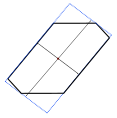
\includegraphics[width=0.8\linewidth]{graphics/surrogate_space}
  \hspace{-5.5mm}
    \end{minipage}
\end{mdframed}
%
As we only need $r$ generators to construct the surrogate space but have $d$ generators of $Z_p$ available, not all $p_i$ are used in the surrogate space construction.
In theory, the generators $p_i$ that are used to calculate the $q_i$ don't have to be ordered.
However, to emphasize the most important generators $p_i$, they are ordered by their magnitude such that $|p_1| \geq \dots \geq |p_d|$.
This is done to achieve the best possible encasement of $Z_p$, which is aligned along the dominant generators with respect to their length.

\subsection{Reduced unit hypercube}
\label{sec:ruh}

The surrogate space $S$, which is already a hypercube, is then transformed into the unit hypercube $\Omega_R$ in the last necessary step.
First, we observe that the generators of $S$ are created using the orthogonal vectors $q_i$ and the scaling factors $s_i$ to obtain the generator matrix,
\begin{equation}
G \coloneqq \begin{bmatrix}
  \\
    g_1 ~ \dots  ~ g_r\\
    \\
  \end{bmatrix}=Q ~ \text{diag}(s_1, \dots, s_r) ~, ~~~
Q \coloneqq \begin{bmatrix}
  \\
    q_1 ~ \dots  ~ q_r\\
    \\
  \end{bmatrix},
\end{equation}
in which the column vectors $g_i=s_i q_i$ are the corresponding generators of $S$.
To bring the elements of the surrogate space into a coordinate system of a unit hypercube, we perform a change of basis on them.
The change of basis formula to transform the $r$-dimensional elements $x_p=p(x)$ of $S$ into a representation $y$ in the new basis $G$ is $x_p=Gy \Leftrightarrow G^{-1} x_p=y$, and we can therefore obtain
\begin{equation}
y=G^{-1} p(x)=\text{diag}\left(\frac{1}{s_1}, \dots, \frac{1}{s_r}\right) ~Q^T p(x),
\label{alignment}
\end{equation}
where we know that, according to \cref{surrogate_space}, $y_i \in [-1,1]$ holds.
Once the inputs are represented in the new basis, we transform the surrogate space into the $r$-dimensional unit hypercube $\Omega_r$ by first scaling $S$ down by $2$ and then uncentering it again to finally obtain the usable transformation function $t_{W_r} \colon \Omega \mapsto \Omega_r$ for an active direction matrix $W_r$ with
\begin{equation}
t_{W_r}(x) = c_r + \frac{1}{2} \text{diag}\left(\frac{1}{s_1}, \dots, \frac{1}{s_r}\right) ~Q^T p(x),
\label{linear_trans}
\end{equation}
which achieves the goal of mapping from $\Omega$ into $\Omega_r$ just through some scaling and centering operations.
This last step of the transformation process that transforms $S$ into a unit hypercube is shown in \cref{fig:aligned}.

\begin{mdframed}[style=style]
\begin{figure}[H]
        \centering
\begin{minipage}{.49\textwidth}
        \centering
  \caption{Visualization of transformation used to obtain the unit hypercube $\Omega_r$ according to \cref{alignment}.
  The outline of the transformed inputs $t_{W_r}(\Omega)$ is coloured in \lightbluecomma the unit hypercube $\Omega_r$ in dotted \darkbluecomma and the origin in \reddot}
  \label{fig:aligned}
    \end{minipage}%
    \begin{minipage}{0.49\textwidth}
        \centering
   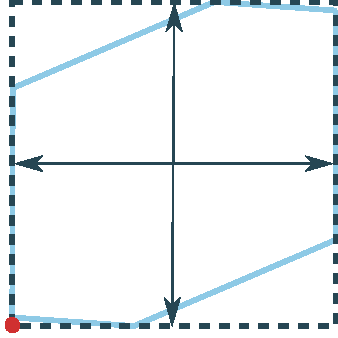
\includegraphics[width=0.7\linewidth]{graphics/surrogate_space_unit}
    \end{minipage}
\end{figure}
\end{mdframed}


\subsection{Visualizing transformations}
\label{sec:vis_trans}

The described transformation process can be visualized by illustrating where points from the lower dimensional space $\Omega_r$ would reside in the original input space $\Omega$.
While it is normally not required to revert the previously shown transformation process, \ie going from $\Omega_r$ back to $\Omega$, it can be useful for the visualization of transformed surrogates.

We observe that \cref{linear_trans} can be rearranged to solve for $p(x)$ with
\begin{equation}
p(x)=2 G (t_{W_r}(x) - c_r)=2 Q ~ \text{diag}(s_1, \dots, s_r) ~ (t_{W_r}(x) - c_r).
\label{proj}
\end{equation}
To reverse the transformation completely, we have to deal with reversing $p(x)$ and the fact that in many cases the inverse function $p^{-1}$ is not injective.
Our goal is to reverse the transformation only onto certain representative elements of the equivalence classes $[x]_p \coloneqq \{x \in \Omega \mid p(x)=x_{p}\}$.
We then only consider the points
\begin{equation}
C \coloneqq \{(x - c_d) \in \text{span} ~ W_r \mid x \in \Omega\},
\label{proj_rep}
\end{equation}
\ie the set of points which lie in the subspace that is spanned by the active directions of $W_r$ and crosses the center $c_d$.
We reverse $p(x)=W_r^T (x-c_d) \Leftrightarrow W_r p(x) + c_d = x$ only onto the representative elements $x \in C$ so that we are able to map one element $x_r \in \Omega_r$ onto one element $x \in C$ to obtain $t_{W_r}^{\text{reverse}}\colon \Omega_r \mapsto C$ with
\begin{equation}
t_{W_r}^{\text{reverse}}(x_r) = ~W_r 2 Q ~ \text{diag}\left(s_1, \dots, s_r\right) (x_r - c_r) + c_d.
\label{trans_rev}
\end{equation}
%
This function is denoted as a reverse function, as it is not a true inverse of $t_{W_r}$.

In \cref{fig:trans_vis}, we can examine the result of reversing the grid points of a regular two-dimensional sparse grid lying in $\Omega_r$ onto a plane in the original three dimensional space $\Omega$ with the help of \cref{trans_rev}.
As we can see, some grid points lie outside of $\Omega$ when being visualized this way.
We will focus on this and other peculiarities inherent to transformations in the next chapter.

\newpage
\begin{mdframed}[style=style]
\vspace{2.5mm}
\begin{figure}[H]
\begin{subfigure}{.5\textwidth}
  \centering
  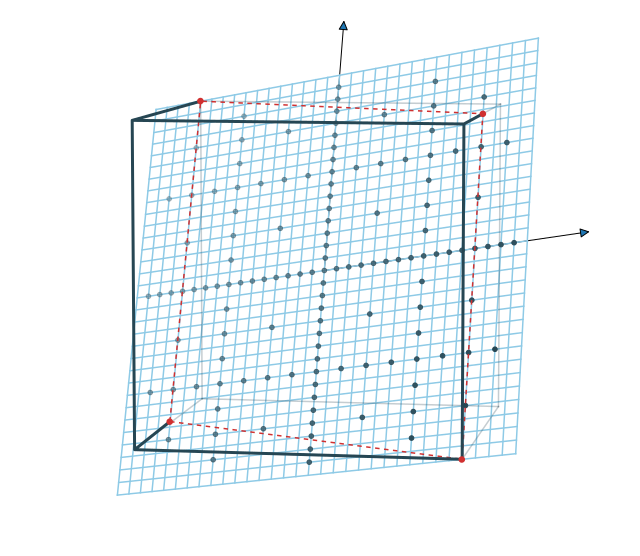
\includegraphics[width=\linewidth]{graphics/surrogate_vis_2}
\end{subfigure}%
\begin{subfigure}{.5\textwidth}
  \centering
  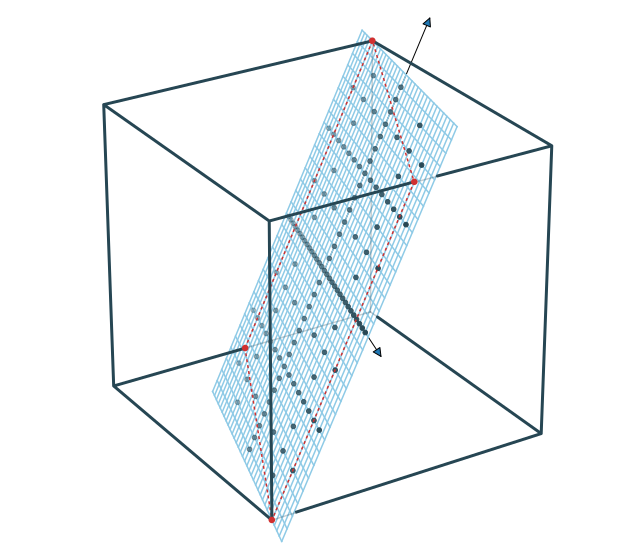
\includegraphics[width=\linewidth]{graphics/surrogate_vis_1}
\end{subfigure}
\vspace{2.5mm}
\delimit
\caption{Two views of the same transformed regular sparse grid of level $5$ with $r=2$ and $d=3$.
The \darkblue cube outline represents the edges of $\Omega$, the arrows are the first two active directions of $W_r$, and the dotted \red lines mark the intersections of $C$ and the edges of $\Omega$.}
\label{fig:trans_vis}
\end{figure}
\end{mdframed}

\section{Active subspaces}
\label{sec:as}

One way to construct the matrix $W_r$, which the foundation of the active direction transformation function $t_{W_r}$, is through the method of active subspaces \cite{Constantine2015}.
This dimensionality reduction technique conducts a parameter study to identify the most influential directions in the input space to construct a lower-dimensional active subspace of $\Omega$ that covers most of the model output variance.
The unused parts of the domain, which are spanned by the leftover inactive directions and are referred to as the inactive subspace, are then cut off.
To obtain the orthonormal active directions, the technique performs a singular value decomposition on the average outer product of the gradients,
\begin{equation}
C \coloneqq \int_{\Omega} (\nabla f) (\nabla f)^T \rho ~ \mathrm{d}x,
\label{eq:as_c}
\end{equation}
a $(d \times d)$ matrix.
Since $C$ is a positive semi-definite matrix, it is possible to decompose it into its eigenvectors $w_i$ and their corresponding real eigenvalues $\lambda_i$ with
\begin{equation}
C = W \Lambda W^T, ~~ \Lambda \coloneqq diag(\lambda_1, \dots, \lambda_d), ~~ W =
  \begin{bmatrix}
  \\
    w_1 ~ w_2 ~ \dots ~ w_{d-1} ~ w_d\\
    \\
  \end{bmatrix},
\end{equation}
where a larger eigenvalue indicates a higher rate of change along the direction.
More precisely, it is the average squared directional derivative of the function with respect to the eigenvector $w_i$ \cite{Constantine2014} with
\begin{equation}
\lambda_i=\mathds{E}\left[\left(\left(\nabla f\right)^T w_i\right)^2\right].
\label{eigenvalues}
\end{equation}
%
We furthermore assume that the eigenvectors in this decomposition are ordered by the magnitude of their eigenvalues, \ie $|\lambda_1| \geq \dots \geq |\lambda_d|$ should hold
Therefore, the column vectors of the matrix $W$ are ordered from the most the active direction $w_1$ to the least active direction $w_d$.
By keeping only a specific amount of the most active directions $r \leq d$, we obtain the active direction matrix with
\begin{equation}
W_r=\begin{bmatrix}
  \\
    w_1 ~ w_2 ~ \dots ~ w_{i-1} ~ w_r\\
    \\
  \end{bmatrix}.
\label{basis}
\end{equation}
%
The active subspace method itself usually determines $r$ by looking at the largest gaps between the eigenvalues to determine suitable cutoff points.
However, we deviate from this approach and will cover the process of determining $r$ later on as the eigenvalue gap approach is not the most optimal choice in the context of this thesis.

To actually compute the active directions, a set of model gradient observations, $S_g \coloneqq \{(x_i, \nabla f(x_i))\}_{i=1}^n$, is used to derive the matrix $C$ with the help of a classical Monte-Carlo approach from \cite{Constantine2014}.
With this approach, the matrix $C$ can be approximated by computing
\begin{equation}
C \approx \frac{1}{n} \sum_{i=1}^n  \left(\nabla f(x_i)\right) \left(\nabla f(x_i)\right)^T.
\label{eq:as_c_approx}
\end{equation}

\subsection{Estimating gradients for active subspaces}
\label{sec:as_est}

One potential downside of the active subspace method is that gradient observations are required to approximate the matrix $C$ in \cref{eq:as_c_approx}.
In cases where the gradient function is not known and can not be easily computed, this would seem like a roadblock limiting the general feasability of the active subspace method.
However, as this section will show, the gradients can be approximated in various ways from available observations and can also be used to obtain an acceptable active subspace approximation.
We will cover a few different methods of achieving this, where each one has its unique advantages and disadvantages as we will see.

\subsection{Finite differences}

The most common approach for estimating gradients of a function are finite differences.
In this thesis, an adaptive mix of forward and backward differences with a fixed distance $h$ are used, where the range of possible spacing is constrained by $0 < h \leq 0.5$.
We can approximate $\nabla f(x)$ with
\begin{equation}
\frac{\partial f(x)}{\partial x_i} \approx
\begin{cases}
    \dfrac{f(x_1, \dots, x_i + h, \dots, x_d) - f(x)}{h}, & x_i + h \leq 1 \\[1.5em]
    \dfrac{f(x_1, \dots, x_i - h, \dots, x_d) - f(x)}{h}, & \text{else}
\end{cases}.
\end{equation}
%
The downside in the context of an observation-based approach is the requirement to additionally evaluate the model function $d$ times to approximate the gradient at one observation sample point $x_i$.
For high values of $d$ and a large amount of observations $n$, additional $dn$ function evaluations for finite differences may become too costly.

\subsection{Directional derivatives}

In cases where finite differences are not suitable, the gradients can be determined using a different approach that only works on a given observation sample and does not require further function evaluations.
The approach is to roughly approximate the gradient by looking at neighbouring observations and using directional derivatives to create a system of linear equations for the gradient at a certain observation point.
Given two inputs $x, y \in \Omega, ~ x \neq y$, the simple approximation rule
\begin{equation}
\langle y-x, \nabla f(x) \rangle \approx f(y) - f(x)
\end{equation}
then just extrapolates the gradient along the direction $y-x$ in a linear fashion.

By choosing $m \in \mathds{N}$ neighbours $N = \{(y_i, f(y_i))\}_{i=1}^m$ of an observation $(x, f(x))$ from the available observation set $S = \{(x_i, f(x_i))\}_{i=1}^n$ with $N \subseteq S \setminus \{(x, f(x))\}$, we can create a system of linear equations with the linear extrapolation approach to obtain
\begin{equation}
\begin{bmatrix}
    y_1 - x\\
    \vdots \\
    y_m - x
  \end{bmatrix}  \widetilde{\nabla} f(x) =\begin{bmatrix}
    f(y_1) - f(x) \\ \vdots \\  f(y_m) - f(x)
    \\
  \end{bmatrix}.
  \label{eq:dd_sle}
\end{equation}
%
Solving this system of linear equations for a residual minimizing value for $\widetilde{\nabla} f(x)$ only provides a very rough approximation of the actual gradient.
Furthermore, the linear nature of the approximation, especially when estimating gradients of a non-linear function, can lead to biased gradients.
The choice of the neighbours $y_i$ also influences the result as well as the amount of neighbours $m$.

In the context of active subspaces, the difference between the approximated gradients and the true gradients is not the relevant metric to evaluate the actual quality of approximated gradients.
Instead, the primary focus should be the resulting surrogate approximation error, as it is the only metric that matters in the end.
Even though the active subspaces computation is based entirely on the average outer product of the gradients, there is not necessarily a strong link between the gradient approximation errors and the quality of the resulting active subspace.
Therefore, the evaluation of the active subspace approximations will be done later on when the surrogate quality in general is investigated.

\paragraph{Random neighbour approximation}
The random neighbour approximation method takes a subset $S_{\text{rn}} \subseteq S \setminus \{(x, f(x))\}$ with $|S_{\text{rn}}|=m < n$ as input.
The set $S_{\text{rn}}=\{(y_i, f(y_i)\}_{i=1}^m$ is then called a random neighbour set of $x$.
This random neighbour set is used as an input for \cref{eq:dd_sle} to compute $\widetilde{\nabla} f(x)$.
Choosing $m \ll n$ can be useful in cases where a lot more observations are available than are necessary for the system of linear equations to return a usable approximation.
This way, the time spent solving the system of linear equations is kept to a minimum.

For $n,m \to \infty$, the approximated gradient does not converge to the actual gradients, since the expected distance to the neighbours in a random neighbour set does not approach zero.
The problem of determining average neighbour distance is related to finding the mean line segment length $\Delta (d)$ in a d-dimensional unit hypercube \cite{Bailey2007}.
There is no closed form solution for $\Delta (d)$, however several approximations have been developed for various dimensionalities in \cite{Weisstein}, \eg $\Delta (1)=\frac{1}{3}$, $\Delta (2)=0.52$, $\Delta (3)=0.66$.
As $\Delta (d)$ grows with the dimensionality $d$, this results in higher average neighbour distances for greater values of $d$.

\paragraph{Nearest neighbour approximation}
The nearest neighbour variant first picks a subset $S' \subseteq S \setminus \{(x, f(x))\}$ with a manageable size $n'=|S'|$ similar to the random neighbour method and then computes the $m \leq n'$ nearest neighbours $S_{\text{nn}}=\{(y_i, f(y_i)\}_{i=1}^m \subseteq S'$ with
\begin{equation}
{\|(y_1-x)\|}_2 < {\|(y_2-x)\|}_2 < \dots < {\|(y_{n'-1}-x)\|}_2 < {\|(y_{n'}-x)\|}_2.
\end{equation}
The obvious advantage is that the used neighbours lie way closer to $x$ than with the random neighbour method.
\Cref{fig:as_approx} illustrates the differences between both methods.

Compared to the random neighbour approximation, for $n,n',m \to \infty$, the approximated gradient does converge to the actual gradient because the expected distance to the neighbours does approach zero.
However, this property comes at the cost of first having to sort the available $n'$ neighbours by distance to pick the $m$ closest ones.
The parameters $n'$ and $m$ also have to be chosen carefully as an unsuitable combination of $n'$ and $m$ would increase the average distance to the neighbours again such that the effect of choosing the nearest neighbours would vanish.

\begin{mdframed}[style=style]
\vspace{2mm}
\begin{figure}[H]
  \centering
\begin{subfigure}{.45\textwidth}
  \centering
  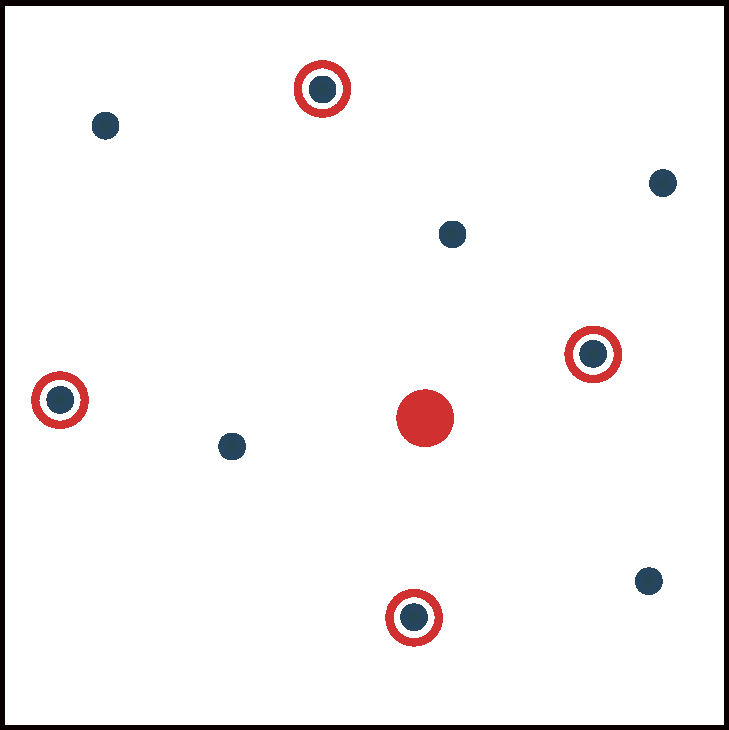
\includegraphics[width=.8\linewidth]{graphics/as_rn}
  \subcaption{Random neighbour method picks with $m=4$.}
  \vspace{2mm}
  \label{fig:as_rn}
\end{subfigure}%
\begin{subfigure}{.45\textwidth}
  \centering
  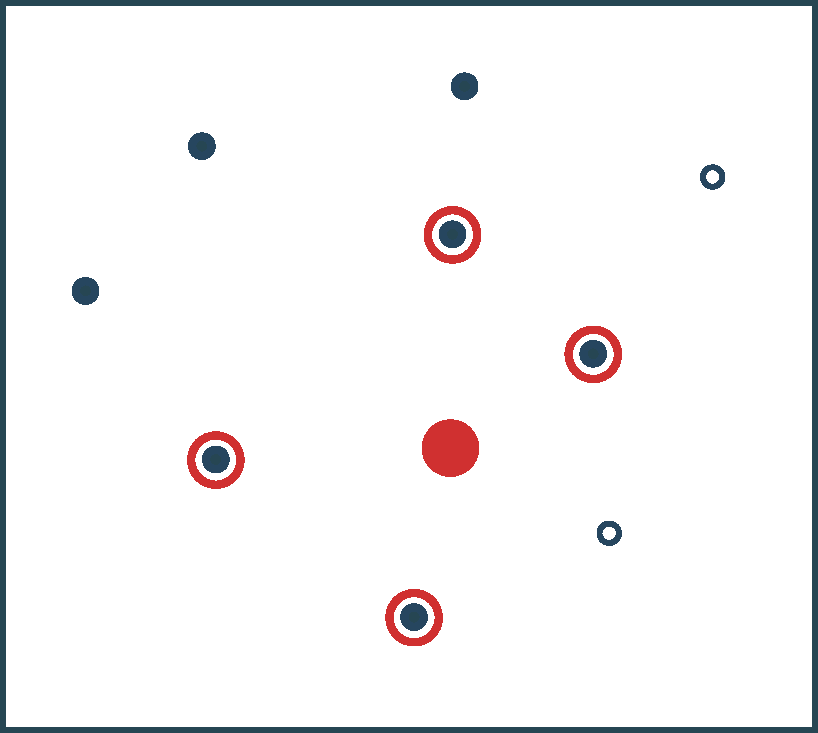
\includegraphics[width=.8\linewidth]{graphics/as_nn}
  \subcaption{Nearest neighbour method picks with $n'=7$ and $m=4$.}
  \vspace{2mm}
  \label{fig:as_nn}
\end{subfigure}
\delimit
\caption{Differences in the neighbour selection between the two neighbour approximation methods for an observation set $S$ with $|S|=10$.
The \darkblue points are the available observations $S \setminus \{(x, f(x))\}$.
A hollow point signals that the observation is not considered when looking for neighbours.
The \red point represents $x$, and other points circled in \red represent observations that were chosen as a neighbour of $x$ by the respective method.}
\label{fig:as_approx}
\end{figure}
\end{mdframed}

\subsection{Limitations}
\label{sec:asl}

Active subspaces, even if the true gradients are used to compute them, are not a perfect indicator on which active directions are suitable for a active direction transformation construction since they can be misled.
According to \cref{eigenvalues}, a larger eigenvalue indicates a higher rate of change along the direction.
More precisely, it represents the average squared directional derivative of $f$ with respect to its eigenvector.
However, a large average squared directional derivative does not necessarily indicate that a direction $v_i$ is worth keeping.
For example, the function
\begin{equation}
f(x_1, x_2)=10x_1 + \frac{1}{10} \sin(100 \pi x_2)
\end{equation}
illustrates the limitations of active subspaces.
The optimal active direction worth keeping would be the first dimension only, as the second term can be seen as a highly changing noise term that does not affect the approximation error a lot if removed as the amplitude of the sine is small.
However, as the average squared directional derivative along the second dimension $(0,1)^T$ is way higher than along the first dimension $(1,0)^T$, the calculated active subspace is biased towards the second dimension.
Therefore, we can not assume that the computed active subspace is always usable as directions with a high rate of change do not always correspond to directions that cover huge portions of the functions output variance.

A positive aspect of the active subspace neighbour approximation methods is that they effectively introduce a regularization through discretization \cite{Kress1999}, \ie as the distances between neighbours are comparatively high, they automatically discard noise terms with high frequencies such as the one shown in the previous example.
In certain cases, this can lead to more suitable active subspace approximation when using neighbour approximation methods compared to alternatives such as the finite differences method.

\section{Random active directions}
\label{sec:rt}

A completely different approach to finding orthonormal active directions $w_i$ to construct a transformation is just generating random ones.
This approach is easy to implement, can generate new transformation functions almost instantly, and offers a purely exploratory way of finding the best transformation.
It can also serve as a reference for comparison as the active subspace method should ideally almost always output better active directions.

A simple generation algorithm first generates random matrices $R \in \mathds{R}^{d \times d}$ until all column vectors are linear independent and then orthonormalizes $R$ using the Gram-Schmidt process to obtain the column vectors with
\begin{equation}
w_i=\frac{w_i'}{\| w_i' \|},~~ w_i'=r_i - \sum_{k=1}^{i-1} \frac{\langle r_k,  w_k' \rangle}{\langle w_k', w_k' \rangle} w_k',
\end{equation}
and therefore the orthonormal active direction matrix
\begin{equation}
W = \begin{bmatrix}
  \\
    w_1 ~ w_2 ~ \dots ~ w_{r-1} ~ w_d\\
    \\
  \end{bmatrix}.
\end{equation}
%
The final step randomly rolls a reduced dimensionality value $r$ with $1 \leq r \leq d$ and cuts off the last $d-r$ column vectors of $W$ to obtain the reduced active direction matrix
\begin{equation}
W_r = \begin{bmatrix}
  \\
    w_1 ~ w_2 ~ \dots ~ w_{r-1} ~ w_r\\
    \\
  \end{bmatrix}.
\end{equation}
%
Note that the generated random orthonormal matrices are not perfectly uniformly distributed in the orthogonal group $O(d)$ and we would need a different algorithm to achieve a true uniform distribution \cite{Wang2008}.
The simple Gram-Schmidt based approach is however perfectly usable for the purpose of generating input transformations.

\section{Alternative transformations}

Until now, the focus lied primarily on active directions because they are relatively easy to use and construct.
However, in theory we can construct and use arbitrary transformation functions to improve the model approximation.
This section will briefly cover a few alternative types of transformations that will not be covered in detail in this thesis but do show some potential that could be investigated further.

\subsection{Periodic transformations}

A possible use case for alternative transformations are periodic functions.
If the model function is for example periodic along one dimension $i$ with the period $p_i$, \ie it holds that $f(x_1,\dots,x_i,\dots,x_d) \approx f(x_1,\dots,x_i + p_i, \dots,x_d)$, we can easily define a transformation function $t_{\text{periodic}} \colon \Omega \mapsto \Omega$ with
\begin{equation}
t_{\text{periodic}}(x_1,\dots,x_i,\dots,x_d) = (x_1,\dots, \frac{x_i\text{ mod } p_i}{p_i}, \dots,x_d)^T,
\label{eq:per}
\end{equation}
and create a surrogate $\hat{f}$ in $\Omega$ with $f(x) \approx \hat{f}(t_{\text{periodic}}(x))$.
This way, the function can be interpolated better by sparse grids since there are effectively $1 / p_i$ times more grid points spent along the $i$-th dimension.
In theory, this concept can be also expanded upon with handling multiple periodic dimensions at once, antiperiodic functions, offsets, and combination with other transformations.

A simple example would be the periodic function $f_{\text{periodic}}(x)=\sin(16\pi x_1)  + \cos(16\pi x_2)$, which repeats in intervals of $\frac{1}{8}$ along both dimensions.
This can be exploited by constructing a periodic transformation with $p=p_1=p_2=\frac{1}{8}$ to obtain
\begin{equation}
t(x_1,x_2) = \left[\frac{1}{p} \left(x_1 \text{ mod } p\right), \frac{1}{p} \left(x_2 \text{ mod } p\right)\right]^T.
\end{equation}
%
To illustrate the improvement of the approximation quality in multiple smaller steps, we investigate periodic a transformation with several periods in \cref{fig:periodic}.
As we can see, a smaller value for $p$ results in a notable improvement, and going from $p=1$ (no transformation) to $p=0.125$ (best periodic transformation) improves the approximation error by a factor of around $10^2$.

\begin{mdframed}[style=style]
\vspace{2mm}
\begin{figure}[H]
        \centering
\begin{minipage}{.35\textwidth}
        \centering
  \captionof{figure}{
  Approximation errors of various periodic transformations with periods $p \in \{\frac{1}{8}, \frac{1}{4}, \frac{1}{2}, 1\}$ in combination with sparse grid surrogates of level $\ell \in \{1, \dots, 11\}$ and modified hat basis functions for the function $f_{\text{periodic}}$.}
\label{fig:periodic}
    \end{minipage}%
    \begin{minipage}{0.65\textwidth}
        \centering
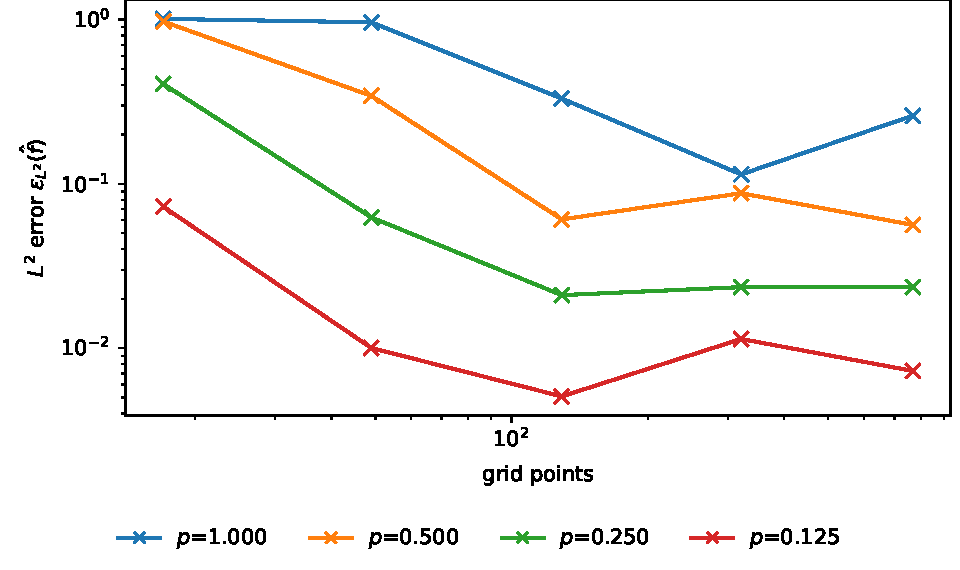
\includegraphics[width=0.85\textwidth]{graphics/periodic}
    \end{minipage}
\end{figure}
\end{mdframed}

\subsection{Manifolds}

Manifold-based methods for dimensionality reduction aim to identify nonlinear subspaces in the domain that are suitable for a dimensionality reduction.
They have the potential to create more flexible transformations compared to active directions but are also harder to implement and make use of.

\paragraph{Active Manifolds}
Inspired from active subspaces, which are purely linear in their nature, we can extend the concept to identifying a one-dimensional curve in the domain $\Omega$ along the flow of most active change, which is called an active manifold \cite{Bridges2019}.
Compared to active subspaces, calculating the active manifold is more complex and resource intensive.
Furthermore, defining a transformation function that maps from $\Omega$ onto the local one-dimensional space of the curve is way more complex and can be constructed in possibly many different ways.
This technique is currently limited to only one dimension with $r=1$, which results in the used surrogate construction method becoming pretty irrelevant.

\paragraph{Principal Manifolds}
A similar concept to active manifolds are principal manifolds \cite{Huo2008}.
They are an extension to principal component analysis \cite{Abdi2010}, which can only compute linear principal components.
The principal manifold technique is able to construct nonlinear multi-dimensional manifolds and is therefore more powerful than active manifolds.
This technique has already been investigated in conjunction with sparse grids in \cite{Feuersaenger2009}.

\chapter{Transformed surrogates}
\label{chap:c4}

Once a transformation function has been created, the next step is creating the surrogate in the reduced input space $\Omega_r$.
As we will see in this chapter, this is not a trivial thing to do with sparse grids and requires special care as there are several hurdles that come with the usage of input transformations.
Some of these are specific to sparse grids, whereas others are independent of the used surrogate type.

\section{Transformed input space}
\label{sec:tis}

All transformed inputs form the transformed input space, which is a part of the reduced input space $\Omega_r$.
In the last chapter, the transformation was constructed in such a way that every transformed input lies in $\Omega_r$ while also applying appropriate scaling to still use as much space of $\Omega_r$ as possible.

\begin{definition}[Transformed input space]
Let $t \colon \Omega \mapsto \Omega_r$ be transformation function.
We define the transformed input space as
\begin{equation}
T \coloneqq \{t(x) \mid x \in\Omega\}, ~~ T \subseteq \Omega_r.
\end{equation}
\end{definition}
%
The main difference between $T$ and $\Omega_r$ is that $\Omega_r$ is a unit hypercube, while $T$ might not be one.
As we will see later on, $T$ is not a unit hypercube in in many cases.
We should strive to have $T$ cover $\Omega_r$ as much as possible to not make a huge portion of $\Omega_r$ go unused when constructing the surrogate.

\begin{definition}[Unused reduced surrogate inputs]
Let $t \colon \Omega \mapsto \Omega_r$ be transformation function, and let $U=T \setminus \Omega_r$ be the unused reduced surrogate space.
We then define
\begin{equation}
\tilde{u}_t \coloneqq \frac{|U|}{|\Omega_r|}
\end{equation}
as the share of unused space in the reduced input space.
\end{definition}
%
The greater $U$, and therefore the unused input share $\tilde{u}_t$, the more grid points of a sparse grid can potentially be generated outside of $T$.
Note that even if a grid point lies outside of $T$, it can still contribute to some degree to the approximation error of the surrogate if the support of the basis function $\phi$ intersects with $T$.
Thus, grid points are only completely unused if their basis function support does not intersect with $T$ at all.
Other surrogate types do not have the same issue as radial basis functions for example can freely choose their support points and therefore automatically adapt to the shape of $T$ in relation to $\Omega_r$.

\section{Method selection}
\label{sec:ms}

Usually, the standard sparse grid technique makes use of interpolation (see \cref{sec:gsc}) and is able to generate an accurate interpolant quickly.
However, as we will show in this section, sparse grid interpolation is not suitable for many scenarios involving transformations and we will have to differentiate between two cases.

\subsection{Interpolation}
If it holds that $r=d$, \ie we do not perform a dimensionality reduction, the transformation can be seen as orientation changing only.
In that case, if an active direction transformation is created according to the rules of the previous chapter such that all inputs are transformed into a unit hypercube with equal dimension, the transformation function is injective and maps from $\Omega$ to $T \subseteq \Omega_r$.
\Cref{fig:aligned_grid} illustrates this case.

\begin{mdframed}[style=style]
\begin{figure}[H]
        \centering
\begin{minipage}{.49\textwidth}
        \centering
  \captionof{figure}{Exemplary case of an active direction transformation with $r=d=2$. The \beige square represents $\Omega=\Omega_r$, the black dots are the grid points of a sparse grid surrogate, and the rotated \lightblue square represents $T$. The \grey square in top right corner represents the basis function support of the grid point in its center.}
\label{fig:aligned_grid}
    \end{minipage}%
    \begin{minipage}{0.49\textwidth}
        \centering
   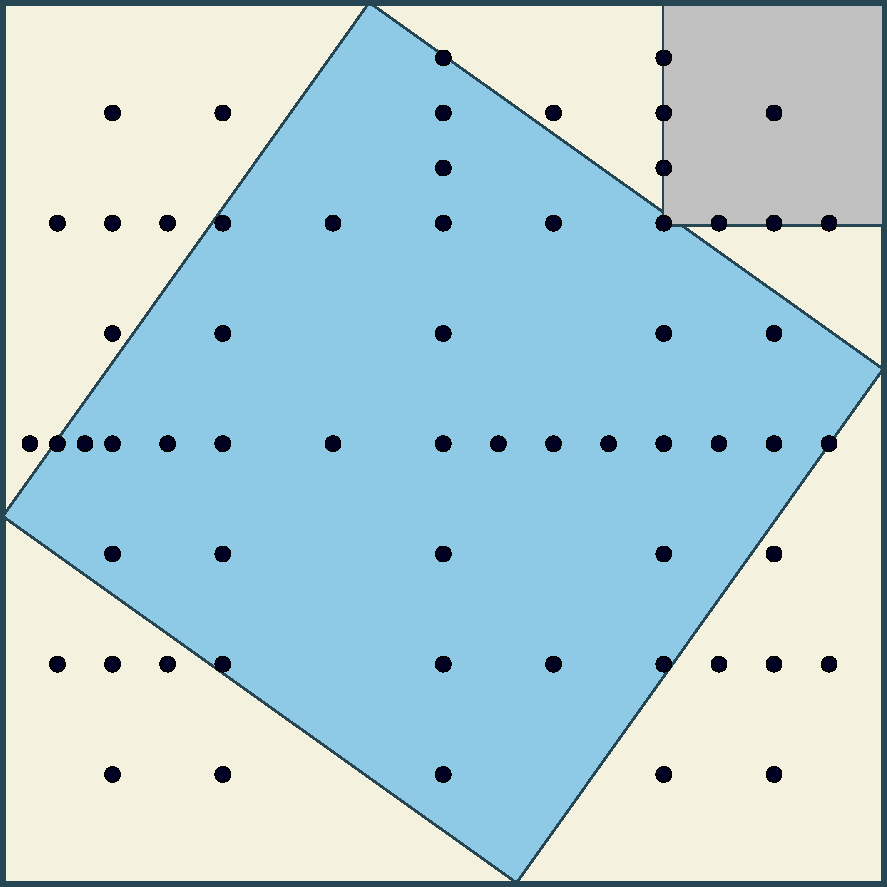
\includegraphics[width=0.8\linewidth]{graphics/aligned_grid}
   \vspace{2mm}
    \end{minipage}
\end{figure}
\end{mdframed}
%
It is then possible to use normal sparse grid interpolation to create a surrogate for the transformation if we define how to treat grid points outside of $T$.
For that we can either ensure that grid points outside of $T$ never are created or define a rule on how to treat these out of domain function evaluations.

Restricting grid point creation in $U$ is difficult as the grid point hierarchy, which dictates that every grid point has a parent, should be kept intact to work effectively with sparse grids.
Thus, restricting grid point creation in $U$ can prevent large areas in $\Omega$ being covered by grid points as a basic parent grid point might lie outside of $T$ and would not be added to the grid.
Note that even if there are many grid points that were generated outside of $T$, as seen in figure \cref{fig:aligned_grid}, very few grid points are actually completely unused as the support of many grid point basis functions intersects at least barely with $T$ and therefore contributes to the overall approximation.

The alternative approach would require us to define rules on how to treat grid points outside of $T$, which when mapped to their corresponding function input, would lie outside of $\Omega$.
To evaluate the model function at a grid point for a transformed sparse grid, we need to inverse the transformation.
As the transformation function is an automorphism of $\Omega$ when $r=d$, it is invertible for elements $t \in T$ and the inverse function $t^{-1} \colon T \mapsto \Omega$ can easily be constructed.
We can also extend the inverse transformation $t^{-1}$ to accept all elements $x \in \Omega_r$ without a problem with $t^{-1}_{\text{ext}} \colon \Omega_r \mapsto \mathds{R}^d$ to be able to inverse a grid point that lies outside of $T$.
In a similar fashion, we also have to extend the model input domain to allow the model function to be evaluated outside of $\Omega$ to create the interpolant surrogate $\hat{f}(x)=f_\text{ext}(t^{-1}_{\text{ext}}(x))$.
A simple implementation could set all values outside of $\Omega$ to 0 with
\begin{equation}
f_{\text{ext}, 0}(x) \coloneqq \begin{cases}
f(x), &\text{if $x \in \Omega$}\\
0, &\text{else}
\end{cases}
\end{equation}
or alternatively just extend the input domain to allow the model function to be evaluated outside of $\Omega$ with $f_{\text{ext}, f}(x) \coloneqq f(x)$.
Whether the latter approach is feasible or not depends on the model function behaviour when leaving the original input domain $\Omega$.

\subsection{Regression}
In case we perform a dimensionality reduction with $r < d$, we can no longer make use of sparse grid interpolation as the transformation is longer invertible.
We are then dealing with data that might be, depending on the model function and the transformation, very noisy and there also might be multiple different values for the same inputs with
\begin{equation}
t(x_i)=t(x_j), ~ f(x_i) \neq f(x_j), ~ x_i \neq x_j.
\end{equation}
As a result, the transformed surrogate construction is usually an ill-posed problem for $r < d$ and we have to employ regression based methods to successfully create a surrogate for the transformed data.
\Cref{fig:reduced_grid} illustrates this case.

\begin{mdframed}[style=style]
\begin{figure}[H]
        \centering
\begin{minipage}{.5\textwidth}
        \centering
  \caption{Exemplary case with $r=1$ and $d=2$.
  The surrounding \beige square represents $\Omega$, the \lightblue line represents $\Omega_r=T$, and the black dots are the grid points of the one-dimensional sparse grid surrogate.
The \green points are observations that are being mapped from $\Omega$ onto $\Omega_r$.
Note that as $\Omega$ and $\Omega_r$ are distinct vector spaces, this figure visualizes the one dimensional $\Omega_r$ as the elements crossing the center in the two-dimensional space.}
\label{fig:reduced_grid}
    \end{minipage}%
    \begin{minipage}{0.5\textwidth}
        \centering
   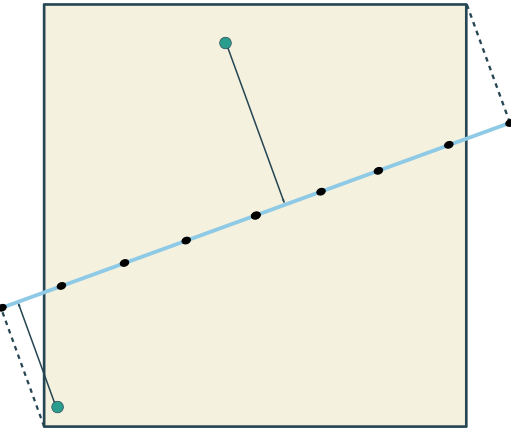
\includegraphics[width=0.85\linewidth]{graphics/reduced_grid}
    \end{minipage}
\end{figure}
\end{mdframed}
%
Since the focus of this thesis lies on dimensionality reducing transformations and the regression approach is also able to handle the orientation changing case with $r=d$, we will primarily use the regression method for the sparse grid surrogate construction.
For this, the original observations,
\begin{equation}
S =\{(x_1, f(x_1), \dots, (x_n, f(x_n))\} \subseteq \Omega \times \mathds{R},
\end{equation}
which were drawn randomly from the given input probability distribution $\rho$, are transformed to obtain the transformed observations,
\begin{equation}
S_t \coloneqq \left\{(t(x_1), f(x_1), \dots, (t(x_n), f(x_n))\right\} \subseteq T \times \mathds{R}.
\end{equation}
We then construct the surrogate $\hat{f}_t$ for the transformed observation set $S_t$ using sparse grid regression (see \cref{sec:gsc}) on a grid point set $X$ and basis functions $\phi_{\underline{l},\underline{i}}$ to obtain the sparse grid surrogate,
\begin{equation}
\hat{f}_t(x) \coloneqq \sum_{x_{\underline{l},\underline{i}} \in X} \alpha_{\underline{l},\underline{i}} \phi_{\underline{l},\underline{i}}(x).
\end{equation}

\section{Multifidelity surrogates}
\label{sec:lofi}

Compared to sparse grid interpolation, the regression method takes longer to construct a well fitting surrogate because an optimization problem that involves all grid points has to be solved.
Furthermore, the regression method also requires parameter calibration since there are many configuration parameters available that can significantly affect the resulting surrogate.
Given a set of possible regression configuration parameter combinations, finding the best combination can become very computationally expensive as every parameter combination has to be evaluated to determine the best one.
To mitigate this problem, we employ the concept of multifidelity simulations \cite{Robinson2006, Forrester2008}, \ie reducing the cost of parametrization by using low-fidelity sparse grids and datasets to evaluate a parameter combination and only using high-fidelity sparse grids and datasets when creating the final surrogate using the determined optimal parameters.

A low-fidelity sparse grid surrogate $\hat{f}^l$ has less grid points and employs no adaptivity compared to a high-fidelity sparse grid surrogate $\hat{f}^h$, \ie the level of $\hat{f}^l$ is lower and no grid points are refined.
It is vital that the used low-fidelity surrogates still stay comparable when evaluating their approximation errors for different parameter combinations.
They don't have to be representative of the high-fidelity approximation error but should be indicative of the comparative quality of their high-fidelity surrogates, \ie it should hold that
\begin{equation}
\varepsilon(\hat{f}_1^l) < \varepsilon(\hat{f}_2^l) \Rightarrow \varepsilon(\hat{f}_1^h) < \varepsilon(\hat{f}_2^h).
\end{equation}
%
This multifidelity approach will also be heavily utilized in later chapters.
The ability to evaluate transformed surrogates quickly is especially critical for random active direction transformation (see \cref{sec:rt}) because it allows for the generation and evaluation of many transformations to choose the best from.

\section{Operations on transformed surrogates}

Now that we are able to construct a transformed surrogate and approximate the model function with $f(x) \approx \hat{f}_t(t(x))$, we can look at the differences when working with transformed sparse grid surrogates compared to using sparse grid interpolation surrogates without employing an input transformation function.

\paragraph{Differentiation}
Assuming that the surrogate uses a basis that can be differentiated easily, such as B-splines, the gradients can be approximated using the chain rule and the gradient function of the transformed surrogate to get
\begin{equation}
\nabla f(x) \approx \nabla \hat{f}_t(t(x)) = \nabla (\hat{f}_t \circ t)(x)=\left(\frac{\partial t(x)}{\partial x}\right)^T \frac{\partial \hat{f}_t(t(x))}{\partial x}.
\end{equation}
Therefore, as long as the transformation function and the surrogate are differentiable, the transformed surrogate can be differentiated as well.
This holds true for the primarily used active direction transformations.

\paragraph{Optimization}
To determine the approximate maximum $x^\text{max} \coloneqq \argmax_{x \in \Omega} f(x)$ or minimum $x^\text{min} \coloneqq \argmin_{x \in \Omega} f(x)$ of the model function, we can perform an optimization on the transformed surrogate in $\Omega_r$.
There already exist optimization algorithms for sparse grids, especially for B-spline basis functions, presented in \cite{Valentin2019}.
However, we have to keep in mind that not every element $x_r \in \Omega_r$ might actually have a corresponding input in $x \in \Omega$ that maps onto $x_r$ with $x_r=t(x)$.
Therefore a constrained optimization has to be performed on the surrogate with
\begin{equation}
x_{r}^\text{max} \coloneqq \argmax_{x_r \in \Omega_r} \hat{f}(x_r), ~ x_r \in T.
\end{equation}
%
Afterwards, at least for dimensionality preserving transformation with $r=d$, we then can obtain the maximum $x^\text{max}$ with $x^\text{max}=t^{-1}(x_{r}^\text{max})$, since $x_{r}^\text{max} \in T$.
One problem is that in the case of a dimensionality reducing transformation with $r<d$, a computed transformed surrogate maximum or minimum may be a set of many points in the original input domain $\Omega$.
Therefore another non sparse grid based optimization has to be performed on the set $t^{-1}(x_{r}^\text{max})=\{x \in \Omega \mid t(x)=x_{r}^\text{max}\}$ to obtain a good maximum estimate.

\paragraph{Quadrature}
Given an input distribution $\rho$ and transformation $t$, we can approximate the integral of the model function with
\begin{equation}
\begin{split}
\int_{\Omega} f(x) \rho(x) \; \text{d}x \approx &\int_{\Omega} \hat{f}_t(t(x)) \rho(x) \; \text{d}x\\
=&\int_{\Omega_r} \hat{f}_t(x_r) \left(\int_{t^{-1}(x_r)} \rho(x)  \; \text{d}x \right)  \; \text{d}x_r\\
=&\int_{\Omega_r} \hat{f}_t(x_r) \rho_t(x_r) \; \text{d}x_r.
\end{split}
\end{equation}
We have to note that the transformed distribution $\rho_t$ is usually a complex distribution, even in cases where $\rho$ is a uniform distribution.
Furthermore, similar to transformed optimization, integration of $\hat{f}_t$ over $\Omega_r$ is not representative in case $\Omega_r \neq T$.
We therefore lose the ability to easily employ sparse grid based quadrature algorithms.
However, since we are aiming to choose $r$ to be a lot smaller than $d$, a Monte-Carlo based quadrature becomes a much better option for transformed surrogates as the curse of dimensionality is weakened that way.

\chapter{Iterative transformations}
\label{chap:c5}

We now covered all the required steps to approximate a model function with a transformed surrogate, which in this thesis mainly happens to be a transformed sparse grid.
However, we can easily see that using just one transformed surrogate for approximation purposes is not as powerful as it needs to be for many models.
Especially if the model function is a sum of terms itself, an iterative approach that generates a sum of multiple different transformed surrogates suits a model function better than a single one.
We can extend the definition of intrinsic dimensionality, to obtain a concept for surrogate sums:
\begin{definition}[Compounded intrinsic dimensionality]
A $d$-dimensional function $f(x_1, \dots, x_d)$ has a compounded intrinsic dimensionality of $r \leq d$ if there exist $p$ transformation functions $t_i \colon \Omega \mapsto \Omega_{r_i}$ and functions $f_{t_i} \colon \Omega_{r_i} \mapsto \mathds{R}$ with $r=\max r_i$ such that
\begin{equation}
\forall x \in \Omega \colon f(x)=\sum_{i=1}^p f_{t_i}(t_i(x)).
\end{equation}
\label{def:intrinsic_sum}
\end{definition}
%
For example, having multiple surrogates allows us to approximate model functions that consist out of multiple terms with a low compounded intrinsic dimensionality such as $f(x_1, x_2)=\sin(2 \pi x_1) + x_2$, which consists out of two terms with an intrinsic dimensionality of $1$ and therefore also a compounded intrinsic dimensionality of $1$.

\section{Projection pursuit regression}

When taking a look at other dimensionality reduction techniques to draw some inspiration from them, one insightful related method that shares some similarities is projection pursuit regression \cite{huber1985projection}.
The projection pursuit regression technique comes from statistics and is in its core idea related to our approach with active direction transformations.
It tries to represent a dataset,
\begin{equation}
P \coloneqq \{(x_i, y_i)\}=\{(x_i, f(x_i))\},
\end{equation}
using the statistical model,
\begin{equation}
y_i=\beta_0 + \sum_{k=1}^m f_k(\beta_k^T x_i) + \varepsilon_i,
\label{eq:ppr}
\end{equation}
where $\beta_0$ is a constant, $\beta_k$ are projection matrices, the $f_k$ are lower dimensional functions, and the $\epsilon_i$ are the residuals.
Using the $\beta_k$ to map inputs onto a lower-dimensional space is very similar to our concept of creating active direction transformations, which is also based on transformation matrices.
The functions $f_k$ and projection matrices $\beta_k$ of this additive model can be computed iteratively by finding a projection and constructing a surrogate repeatedly for the current error function,
\begin{equation}
e_k(x) \coloneqq f(x) - \sum_{i=1}^k f_k(\beta_k^T x).
\end{equation}
%
A basic implementation of this approach can be seen in \cref{alg:ppr}.

\begin{mdframed}[style=algstyle,frametitle={\textbf{function} \texttt{projectionPursuitRegression}{$(f, k_{\text{max}})$}}]
\normalsize
\vspace{5.5mm}
\begin{algorithmic}[1]

    \State $e_0 = f$
    \For{$k = 1, \dots, k_{\text{max}}$}
    	\State $\beta_k \gets$ \texttt{determineBestProjection}($e_{k - 1}$)
    	\State $f_k \gets$ \texttt{constructBestSurrogate}($e_{k - 1}, \beta_k$)
    	\State $e_k \gets e_{k - 1} - f_k$
    \EndFor
    \State $\hat{f}(x) \gets \sum_{k=1}^m f_k(\beta_k^T x)$
    \State \Return{$\hat{f}$}
\end{algorithmic}

\vspace{-1.5mm}
\delimit

	\captionof{algorithm}{Pseudocode of the iterative projection pursuit regression algorithm. Parameters are the model function $f$ and the maximum amount of iterations $k_{\text{max}}$.}
	\label{alg:ppr}
\end{mdframed}
%
Alternatively, we could also introduce an error exit condition to \cref{alg:ppr} that exits the loop if the approximation error is small enough with $\varepsilon(e_i) < \varepsilon_{\mathrm{min}}$.
We can already spot that the function \texttt{determineBestProjection} relates to \cref{chap:c3} where we extensively covered finding a suitable active direction transformation.
Furthermore, \texttt{constructBestSurrogate} relates to \cref{chap:c4} that covered the creation of sparse grid surrogates for a given transformation.

\section{An iterative approach}
\label{sec:it}

Going from this statistical model to our function approximation problem, we can formulate the same concept using the notation used in this thesis by removing the constant term $\beta_0$ and the residuals $\varepsilon_i$ from \cref{eq:ppr} to get
\begin{equation}
\hat{f}(x)=\sum_{i=1}^m \hat{f_{t_i}}(t_i(x_i)),
\end{equation}
%
where the $t_i$ are active direction transformations, which are similar to the projections $\beta_k^T$ and the $\hat{f_{t_i}}$ are the surrogate equivalents of the $f_k$.
The functions $\hat{f_{t_i}}$ and transformations $t_i$ can then be constructed iteratively by repeatedly executing a stepwise algorithm of first finding a transformation and then constructing a surrogate for the current error function,
\begin{equation}
e_k(x)=f(x) - \sum_{i=1}^k \hat{f_{t_i}}(t_i(x)).
\end{equation}
%
\Cref{alg:itappr} illustrates this iterative approach, which is similar to \cref{alg:ppr}, but has been adapted to fit our notation.
It also handles the error function observations $S_i$ and transformed observations $S_{t_i}$ that are needed to construct a regression surrogate.
The algorithm also includes a flexible exit condition in the form of the function \texttt{shouldExit()}.
We usually either use a fixed amount of iterations exit condition or a relative convergence condition, which exits the loop if the new approximation error has not improved by a certain amount compared to the last iteration, \ie it quits if $\varepsilon(e_i) > (1 - \eta) \varepsilon(e_{i - 1})$ for some $\eta \in [0,1]$.

\newpage
\begin{mdframed}[style=algstyle,frametitle={\textbf{function} \texttt{transformedSurrogateSum}{($f, n$)}}]
\normalsize
\vspace{5.5mm}
\begin{algorithmic}[1]
    \State $e_0 \gets f$
    \State $S_0 \gets \{\left(x_j, e_0(x_j)\right) \mid x_j \sim \rho \}_{j=1}^n$
    \State $\hat{f} \gets 0$
    \For{$i = 1, \dots,  \infty$}
    	\State $t_i \gets$ \texttt{generateBestTransformation}($S_{i - 1}$)
    	\State $S_{t_i} \gets \left\{\left(t_i(x_j), e_{i - 1}(x_j)\right)\right\}_{j=1}^n$
    	\State $\hat{f}_{t_i} \gets$ \texttt{generateBestSurrogate}($S_{t_i}, t_i$)
    	\State $e_i \gets e_{i - 1} - \left(\hat{f}_{t_i} \circ t_i\right)$
    	\State $S_i \gets \{\left(x_j, e_{i - 1}(x_j) - \hat{f}_{t_i}\left(t_i(x_j)\right)\right)\}_{j=1}^n$
    	\State $\hat{f} \gets \hat{f} + \left(\hat{f}_{t_i} \circ t_i\right)$
    	\If{\texttt{shouldExit}$(S_{t_i})$}
    		\State  \textbf{\texttt{break}}
    	\EndIf
    \EndFor
    \State \Return{$\hat{f}$}
\end{algorithmic}
\vspace{-1.5mm}
\delimit
	\captionof{algorithm}{Pseudocode of the iterative transformed surrogate sum algorithm. Parameters are the model function $f$ and the amount of used observations $n$.}
	\label{alg:itappr}
\end{mdframed}
%
Note that this algorithm can be applied to problems where either the original model function or only model observations are given.
The continuous error function $e_i$ is maintained and available in the algorithm only in case $f$ is known.
It is however not required in case only the input observations $S_0$ are given instead of $f$ .

\section{Generating the best surrogate}
\label{sec:gs}

Surrogates can, depending on their type, have possibly many independent configuration parameters that can heavily influence the end result and therefore the approximation error.
The amount of possible configuration parameter combinations makes finding the best combination difficult as it would require the examination of a lot of combinations.
In most cases, the actual surrogate has to be constructed with a given parameter combination to evaluate the suitability of them.
The main driver of the runtime of the function \texttt{generateBestSurrogate} is therefore the amount of configuration parameters available.
Common configuration parameters usually include various regression parameters, with the smoothing factor $\lambda$ being the most prominent one.
More formally, assuming that we have $m$ independent configuration parameters where each one has a set of possible values $C_i$, the combined configuration set would be $C=C_1 \times \dots \times C_m$ and the amount of necessary examinations would be $|C|=|C_1| \dots |C_m|$.

Furthermore, the general structure and properties of the current regression problem at hand can change with each new iteration and the current error function $e_i$.
Thus, configuration parameters have to examined in every iteration again because there might not exist a set of optimal configuration parameters for all iterations.

As a result, low-fidelity surrogates are employed during the parametrization phase that occurs right before the actual high-fidelity surrogate construction.
\Cref{alg:bestsur} shows a simple implementation that uses low-fidelity surrogates for parameter evaluation to reduce runtime to determine the optimal low-fidelity configuration,
\begin{equation}
c^\ast \coloneqq \argmin_{c \in C} \varepsilon(\hat{f}_c^l).
\end{equation}
%
This algorithm works fine presuming that the low-fidelity surrogates $\hat{f}_c^l$ are representative of the high-fidelity ones as already discussed in \cref{sec:lofi}.
It is satisfactory as long as the actual approximation quality of the generated high-fidelity surrogate is close to the optimal configuration over all parameter combinations, \ie in a high-fidelity setting it should hold that
\begin{equation}
\varepsilon(\hat{f}_{c^\ast}^h) \approx \argmin_{c \in C} \varepsilon(\hat{f}_c^h),
\end{equation}
where $c^\ast$ was determined with low-fidelity surrogates.

\begin{mdframed}[style=algstyle,frametitle={\textbf{function} \texttt{generateBestSurrogate}{$(S_{t_i}, t_i)$}}]
\normalsize
\vspace{5.5mm}
\begin{algorithmic}[1]
    \State $c^\ast \gets ?$
    \State $\varepsilon_{min} \gets \infty$
    \For{$c \in C$}
      \State $\hat{f}_c^l$ $\gets$ \texttt{generateLowFidelitySurrogate}($S_{t_i}, t_i, c$)
    	\State $\varepsilon \gets \varepsilon_{S_{t_i}}(\hat{f}_c^l)$
    	\If{$\varepsilon < \varepsilon_{min}$}
    	  \State $\varepsilon_{min}\gets \varepsilon$
    	\State $c^\ast \gets c$
    	\EndIf
    \EndFor
    \State \Return{\texttt{generateHighFidelitySurrogate}($S_{t_i}, t_i, c^\ast$)}
\end{algorithmic}
\vspace{-1.5mm}
\delimit
	\captionof{algorithm}{Pseudocode of the surrogate generation algorithm. The parameters are the current error function observations $S_{t_i}$ and the transformation function $t_i$. The the set of possible surrogate configurations $C$ and Monte-Carlo-based error metric $\varepsilon_{S_{t_i}}$ are fixed.}
	\label{alg:bestsur}
\end{mdframed}
%
Some other sparse grid construction properties, like the level, also have to be adapted to handle arbitrary surrogate dimensionalities as a the approximate grid point amount should be decoupled from the used dimensionality $r$, especially when comparing surrogates with differing dimensionalities.
This means that instead of passing a fixed level $\ell$ when constructing a sparse grid surrogate, we instead specify a fixed grid point amount to control how much grid points the surrogate should approximately have and determine the most appropriate level and refinements from there.
That way, we can always get reasonably close to a specific amount of grid points even for higher dimensionalities.
This means that we can always come reasonably close to any specified grid point amount through choosing the right level and performing the right amount of refinements such that we can accurately compare approximation errors of sparse grid surrogates across all possible reduced dimensionalities because their grid point amount is equal.


\section{Generating the best transformation}
\label{sec:trans_gen}

Until now, we assumed that the reduced dimensionality value $r$ was given and did not cover ways on how to determine the optimal reduced dimensionality $r^\ast$ during each iteration step.
When covering active subspaces in \cref{sec:as}, we already mentioned that, even though the active subspace method provides a suggested criterion to determine the optimal cutoff dimension $r^\ast$ by looking for the largest gap in the sequence of eigenvalues, this criterion is not always optimal and could be influenced by various factors.
Furthermore, alternative transformation generation methods, like random active direction transformations in \cref{sec:rtg}, can not make use of such a cutoff criterion.
We are therefore looking a for a generalized approach to determine the best value for $r^\ast_i$ in each iteration that is independent of the employed transformation type.
One solution would be to use the exploratory look ahead approach, which we already used to find the best configuration parameters in previous section, to determine the best value for $r^\ast_i$ in the same way.
In \cref{alg:besttrans}, we can see a simple implementation to generate the best transformation by testing a range of possible values for $r$.

\begin{mdframed}[style=algstyle,frametitle={\textbf{function} \texttt{generateBestTransformation}{$(S_{i - 1}, r_{\text{min}} ,r_{\text{max}})$}}]
\normalsize
\vspace{5.5mm}
\begin{algorithmic}[1]
    \State $t_i^\ast \gets ~ ?$
    \State $\varepsilon_{min} \gets \infty$
    \For{$r = r_{\text{min}},\dots,r_{\text{max}}$}
      \State $t_{i, r}$ $\gets$ \texttt{generateTransformation}($S_{i - 1}, r$)
      \State $\hat{f}_{c^\ast}^h$ $\gets$ \texttt{generateBestSurrogate}($S_{i - 1}, t_{i, r}$)
    	\State $\varepsilon \gets \varepsilon_{S_{i - 1}}(\hat{f}_c^h)$
    	\If{$\varepsilon < \varepsilon_{min}$}
    	  \State $\varepsilon_{min}\gets \varepsilon$
    	\State $t_i^\ast \gets t_{i, r}$
    	\EndIf
    \EndFor
    \State \Return{$t_i^\ast$}
\end{algorithmic}
\vspace{-1.5mm}
\delimit
	\captionof{algorithm}{Pseudocode of the transformation generation algorithm. Parameters are the error function observations $S_{i - 1}$, the minimum reduced dimensionality $r_{\text{min}}$, and the maximum reduced dimensionality $r_{\text{max}}$.}
	\label{alg:besttrans}
\end{mdframed}
%
The actual implementation of the function \texttt{generateTransformation} is usually fixed and can use any of the transformation generation methods presented in \cref{chap:c3}, for example random active direction transformations.

\newpage
\section{Visualizing the algorithm}

The iterative algorithm can be visualized using a simple two-dimensional function,
\begin{equation}
f(x_1, x_2)=e^{x_1' + 1} + \sin(2 \pi x_2') + 1, ~~ \begin{pmatrix}
    x_1' \\ x_2'
    \\
  \end{pmatrix} = \begin{pmatrix}
    +\cos(0.1 \pi) & -\sin(0.1 \pi)\\
    +\sin(0.1 \pi) & +\cos(0.1 \pi)
    \\
  \end{pmatrix}\begin{pmatrix}
    x_1 \\ x_2
    \\
  \end{pmatrix},
\end{equation}
where the first component contributes the most to the total function value while the second one does not.
It has a compounded intrinsic dimensionality of $1$ and is not axis-aligned to further visualize how the algorithm handles multiple non axis-aligned function terms.

For every iteration, we take a look at the error functions $e_{i - 1}$ and at the regression problem that has solved by the surrogate generator.
To better illustrate the surrogate construction, $r$ is always set to $1$, regardless of whether a value of $r=2$ would make sense or not.
Furthermore, the regression surrogate employs heavy regularization and is only plotted as far as it needs to be, \ie the plot might not cover $[0,1]$ as the amount of transformed samples in the boundary regions is very low.
This also illustrates how the transformed input distribution changes from the original input distribution, a uniform distribution in this case.
The active subspaces gradient inputs were approximated using finite differences, and the amount of samples $n$ is set to $4000$.

As we can see in \cref{fig:pipeline_1}, the first algorithm iteration removes a big chunk of the original function error of $e_0=f$ to reduce the approximation error in the first step.
It identified the most active direction mostly right, constructed a one-dimensional active direction transformation, and was able to create a well fitting regression surrogate for the transformed observations $S_{t_1}$.
The regression surrogate had to employ a lot of regularization, as seen in \cref{fig:pipeline_local_1}, since there is still some function output contribution by the sine term that will all be projected onto the first active direction.
\begin{mdframed}[style=style]
\begin{figure}[H]
\begin{subfigure}{.5\textwidth}
  \centering
  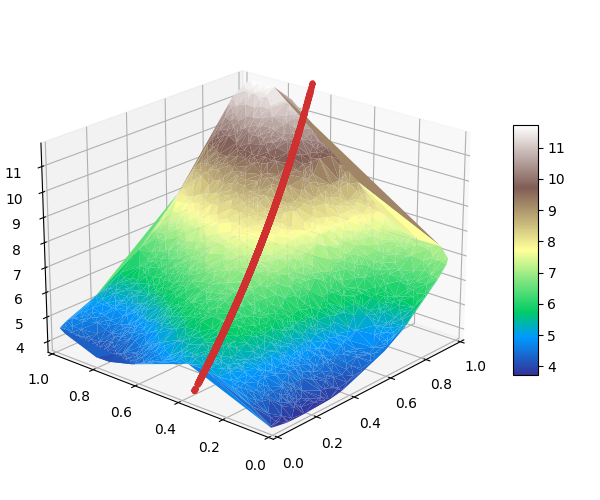
\includegraphics[width=.8\linewidth]{graphics/pipeline_current_1.png}
  \caption{Error function $e_0$ and its intersection with the first active subspace direction $w_1$ in \reddot}
\label{fig:pipeline_current_1}
\end{subfigure}%
\begin{subfigure}{.5\textwidth}
  \centering
  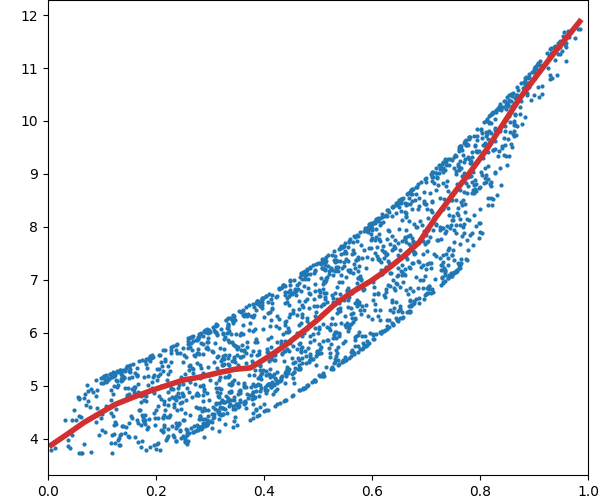
\includegraphics[width=.8\linewidth]{graphics/pipeline_local_1.png}
  \caption{Transformed input samples $S_{t_1}$ in \blue and the surrogate $\hat{f}_{t_1}$ in \reddot}
\label{fig:pipeline_local_1}
\end{subfigure}
\delimit
\caption{First iteration of the iterative transformation algorithm.}
\label{fig:pipeline_1}
\end{figure}
\end{mdframed}
%
In \cref{fig:pipeline_2}, we can clearly identify the remnants of the rotated sine term that are the leftovers after the exponential term was mostly removed in the first iteration.
However, we can also see that the leftover error function is not exactly equal to the sine term as there still exists some noise.
In theory, an optimal method should be able to approximate $f$ without a resulting in a leftover error function after two iterations since it consists out of two terms and its compounded intrinsic dimension is $1$.
However, because the method is not perfect and encounters small errors from various sources throughout the algorithm, it can not approximate functions in an optimal way.
\begin{mdframed}[style=style]
\begin{figure}[H]
\begin{subfigure}{.5\textwidth}
  \centering
  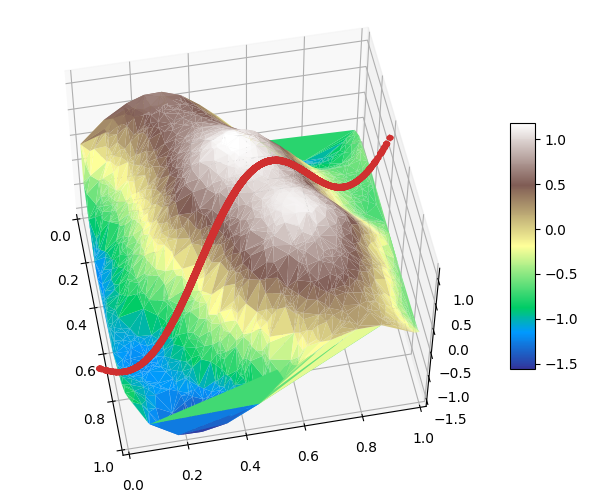
\includegraphics[width=.8\linewidth]{graphics/pipeline_current_2.png}
  \caption{Error function $e_1$ and its intersection with the first active subspace direction $w_1$ in \reddot}
\label{fig:pipeline_current_2}
\end{subfigure}%
\begin{subfigure}{.5\textwidth}
  \centering
  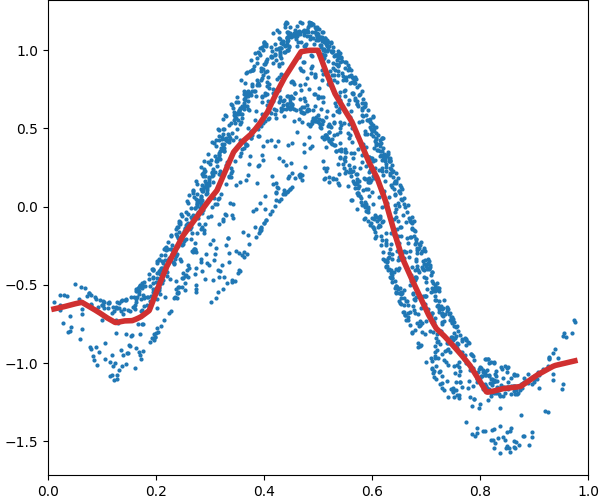
\includegraphics[width=.8\linewidth]{graphics/pipeline_local_2.png}
  \caption{Transformed observations $S_{t_2}$ in \blue and the surrogate $\hat{f}_{t_2}$ in \reddot}
\label{fig:pipeline_local_2}
\end{subfigure}
\delimit
\caption{Second iteration of the iterative transformation algorithm.}
\label{fig:pipeline_2}
\end{figure}
\end{mdframed}
%
These small errors are caused by inaccuracies inherent to the algorithm:
\begin{itemize}
\item The active subspace method not finding perfect active directions caused by the nature of the active subspace method itself (see \cref{sec:asl})
\item The gradient inputs for the active subspace method being biased caused by using gradient approximation methods
\item The regression method not producing ideal surrogates caused by too little or too much regularization or insufficient samples at the boundaries, as seen in \cref{fig:pipeline_local_1} at the left boundary
\end{itemize}
%
As evident in \cref{fig:pipeline_3} and \cref{fig:pipeline_4}, the algorithm eventually hits a point where it can no longer effectively reduce the approximation error by adding another one-dimensional surrogate because the transformed input data is mostly two-dimensional noise that can't be regressed.
Even though we can try to fit a heavily regularized surrogate to the transformed observations, the gain is minimal.
\begin{mdframed}[style=style]
\begin{figure}[H]
\begin{subfigure}{.5\textwidth}
  \centering
  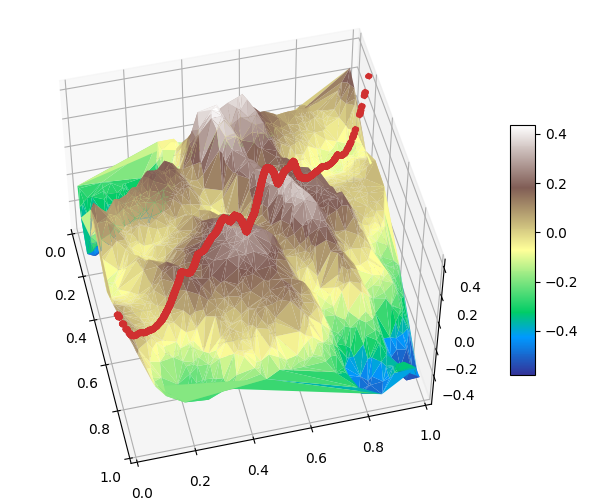
\includegraphics[width=.73\linewidth]{graphics/pipeline_current_3.png}
  \caption{Error function $e_2$ and its intersection with the first active subspace direction $w_1$ in \reddot}
\end{subfigure}%
\begin{subfigure}{.5\textwidth}
  \centering
  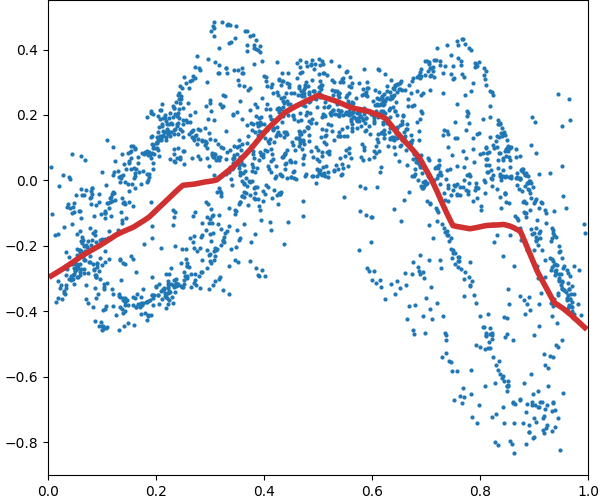
\includegraphics[width=.73\linewidth]{graphics/pipeline_local_3.png}
  \caption{Transformed input samples $S_{t_3}$ in \blue and the surrogate $\hat{f}_{t_3}$ in \reddot}
\end{subfigure}
\delimit
\caption{Third iteration of the iterative transformation algorithm.}
\label{fig:pipeline_3}
\end{figure}
\end{mdframed}
\begin{mdframed}[style=style]
\begin{figure}[H]
\begin{subfigure}{.5\textwidth}
  \centering
  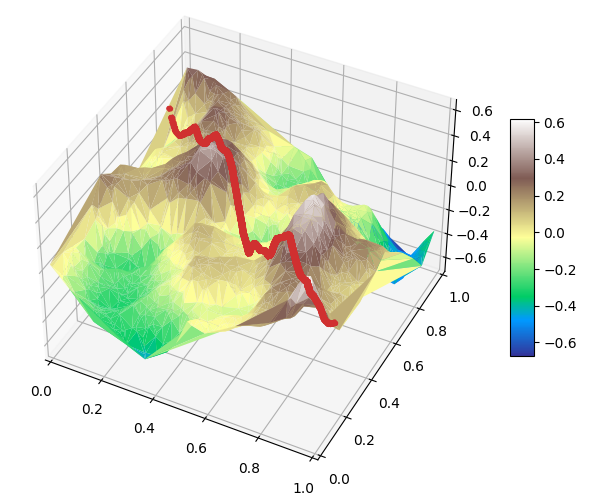
\includegraphics[width=.75\linewidth]{graphics/pipeline_current_4.png}
  \caption{Error function $e_3$ and its intersection with the first active subspace direction $w_1$ in \reddot}
\end{subfigure}%
\begin{subfigure}{.5\textwidth}
  \centering
  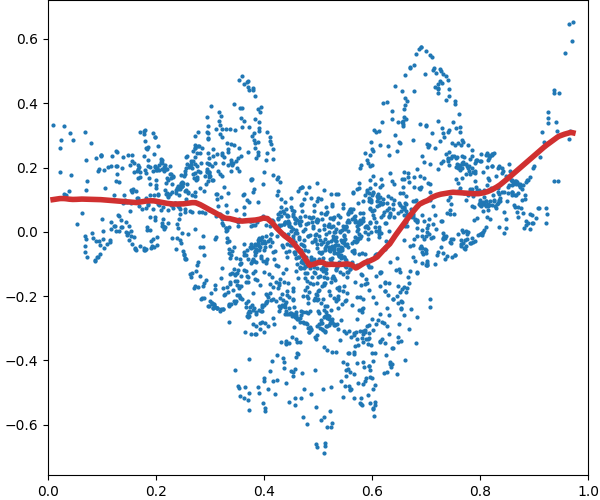
\includegraphics[width=.75\linewidth]{graphics/pipeline_local_4.png}
  \caption{Transformed input samples $S_{t_4}$ in \blue and the surrogate $\hat{f}_{t_4}$ in \reddot}
\end{subfigure}
\delimit
\caption{Fourth iteration of the iterative transformation algorithm.}
\label{fig:pipeline_4}
\end{figure}
\end{mdframed}
%
In \cref{fig:pipeline_5}, we observe that we definitely hit a convergent state as the change compared to the previous iteration is minimal again.
Therefore, we stop the algorithm after this iteration and return a sum of five one-dimensional sparse grid surrogates as an approximation for the model function.
We can also choose to not include the last few transformed surrogates as they did not vastly improve the approximation.
\begin{mdframed}[style=style]
\begin{figure}[H]
\begin{subfigure}{.5\textwidth}
  \centering
  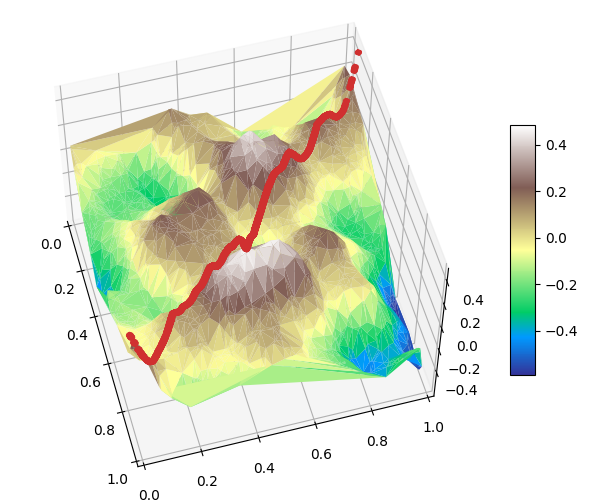
\includegraphics[width=.8\linewidth]{graphics/pipeline_current_5.png}
  \caption{Error function $e_4$ and its intersection with the first active subspace direction $w_1$ in \reddot}
\end{subfigure}%
\begin{subfigure}{.5\textwidth}
  \centering
  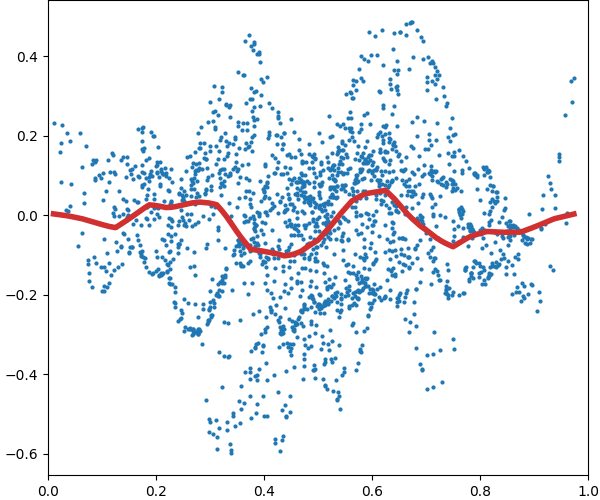
\includegraphics[width=.8\linewidth]{graphics/pipeline_local_5.png}
  \caption{Transformed input samples $S_{t_5}$ in \blue and the surrogate $\hat{f}_{t_5}$ in \reddot}
\end{subfigure}
\delimit
\caption{Fifth iteration of the iterative transformation algorithm.}
\label{fig:pipeline_5}
\end{figure}
\end{mdframed}

\section{Local vs global optimization}
\label{sec:lvsg}

The previously introduced transformation generation algorithm uses a local optimization approach to determine the optimal transformation to use.
However, in some cases this approach can lead the algorithm down a wrong path that will result in a worse approximation error in the end than otherwise possible.
If we look at the example function from the previous section again and give the algorithm the additional choice of not employing a lot of regularization, the algorithm might fall in to the trap of overfitting when only looking ahead one iteration.
\begin{mdframed}[style=style]
\begin{figure}[H]
\begin{subfigure}{.5\textwidth}
  \centering
  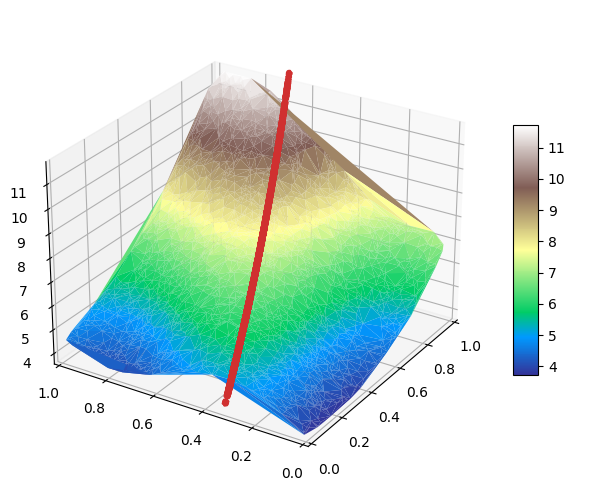
\includegraphics[width=.75\linewidth]{graphics/pipeline_bad_current_1.png}
  \caption{Error function $e_0=f$ and its intersection with the first active subspace direction $w_1$ in \reddot}
\label{fig:pipeline_bad_current_1}
\end{subfigure}%
\begin{subfigure}{.5\textwidth}
  \centering
  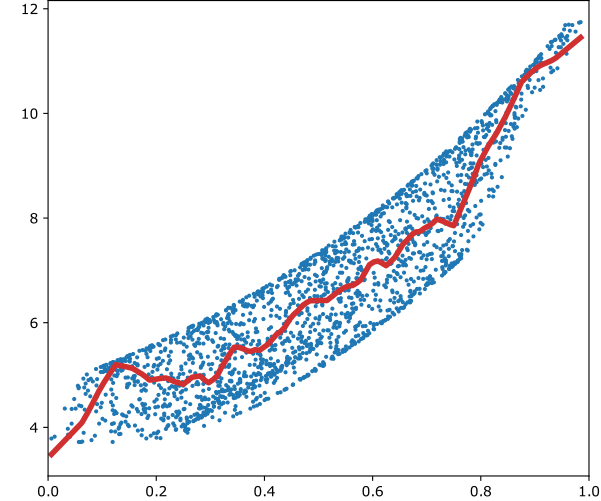
\includegraphics[width=.75\linewidth]{graphics/pipeline_bad_local_1.png}
  \caption{Transformed input samples $S_{t_1}$ in \blue and the surrogate $\hat{f}_{t_1}$ in \red.}
\label{fig:pipeline_bad_local_1}
\end{subfigure}
\delimit
\caption{First iteration of the iterative transformation algorithm with less regularization than before.}
\label{fig:pipeline_bad_1}
\end{figure}
\end{mdframed}
%
As we can see in \cref{fig:pipeline_bad_local_1}, the surrogate is overfitted.
At this stage, the approximation error is almost equal to the more regularized surrogate from \cref{fig:pipeline_local_1} due to the noise.
However, the consequences of this badly fitted surrogate will propagate into the next iteration.
\Cref{fig:pipeline_bad_local_2} shows that no effective surrogate can be created as the input data is mostly just noise because the surrogate in the previous iteration was overfitted.

\begin{mdframed}[style=style]
\begin{figure}[H]
\begin{subfigure}{.5\textwidth}
  \centering
  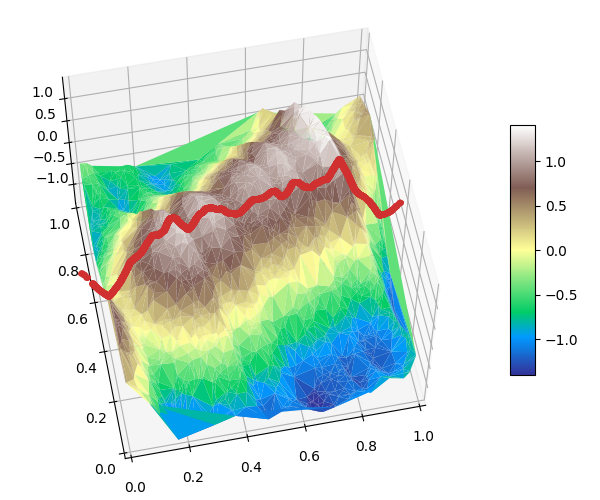
\includegraphics[width=.85\linewidth]{graphics/pipeline_bad_current_2.png}
  \caption{Error function $e_1$ and its intersection with the first active subspace direction $w_1$ in \reddot}
\label{fig:pipeline_bad_current_2}
\end{subfigure}%
\begin{subfigure}{.5\textwidth}
  \centering
  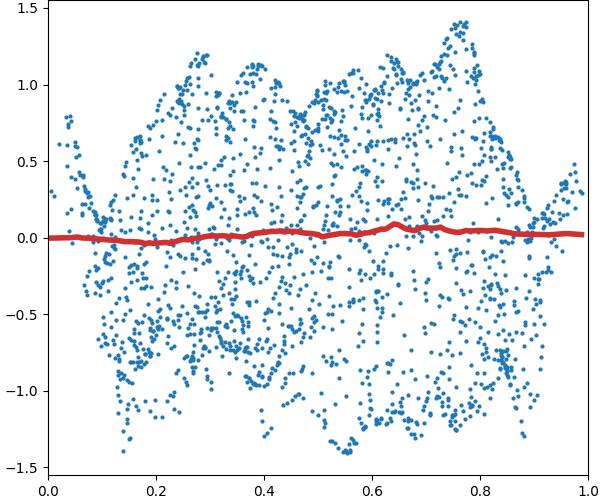
\includegraphics[width=.85\linewidth]{graphics/pipeline_bad_local_2.png}
  \caption{Transformed input samples $S_{t_2}$ in \blue and the surrogate $\hat{f}_{t_2}$ in \red.}
\label{fig:pipeline_bad_local_2}
\end{subfigure}
\delimit
\caption{Second iteration of the iterative transformation algorithm with less regularization than before.}
\label{fig:pipeline_bad_2}
\end{figure}
\end{mdframed}
%
One solution would be to instead look ahead more than iteration in cases where overfitting is possible.
Instead of effectively performing only one look ahead iteration, we could perform $i$ look ahead iterations to better gauge the quality of the produced transformation with regards to the resulting approximation error of the surrogate sum.
To guarantee fast execution speed, we would have to use low-fidelity surrogates when looking ahead.

A more simple solution would be to just very carefully treat the smoothing factor $\lambda$ and prefer more regularization over less regularization.
However, this might not deliver optimal results as in some cases, especially if the last iteration is performed, a lower regularization factor might deliver better results.

\chapter{Implementation}
\label{chap:c6}

The last step missing before we can apply the transformed sparse grid technique to practical models is the actual implementation since all required theoretical aspects have been covered.
In this chapter, we will take a look at the practical implementation of the iterative algorithm described in \cref{chap:c5} and model its various components using component diagrams to describe the general structure and possible configuration parameters.
Such a formal description of the whole implementation will make the experimental results presented later as transparent as possible because it will list and explain possible algorithm configuration parameters that will impact the end result.
The used notation for these component diagrams is shown in \cref{fig:defs}.

\begin{mdframed}[style=style,frametitle={Notation}]
\begin{figure}[H]

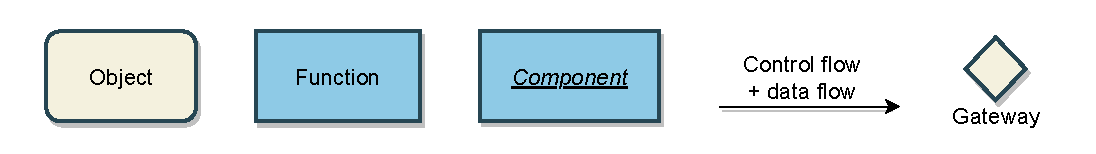
\includegraphics[width=\textwidth]{graphics/definitions.pdf}
\vspace{-7.5mm}

\delimit

\vspace{3.5mm}

\begin{description}
\item[Elements] {~ \begin{itemize}[\null]
\item \textbf{Object}: An object can represent any kind of data, for example a model function, a set of function observations, a transformation function, a surrogate, and more.
\item \textbf{Function}: A function takes some inputs in the form of objects, performs some kind of operation on them, and outputs an object.
\item \textbf{Function component}: A function component is a also function where the actual implementation can be exchanged for many different function implementations of the same interface.
\item \textbf{Control flow + data flow}: Arrows signal control flow and also data flow.
\item \textbf{Gateway}: A gateway evaluates an attached condition and decides which outgoing control flow to follow.
\end{itemize}}
\end{description}

\delimit

\caption{Notation used for different elements in the component structure diagrams in this chapter.}
\label{fig:defs}
\end{figure}
\end{mdframed}
%
The source code of this project, which internally is called \textit{tsgpp} as it adds transformations to the $\mathrm{SG}^{++}$ library \cite{Pflueger2010}, is publicly available at \href{https://github.com/crschnick/tsgpp}{https://github.com/crschnick/tsgpp}.
It is basically implemented exactly as described in this chapter.

\newpage
\section{Transformation pipeline}
\label{sec:tp}

The complete transformation process is modeled and implemented as pipeline that is made up of different components to allow for maximum flexibility.
The pipeline structure is visualized in \cref{fig:tp}.
Every pipeline iteration has the goal of adding another transformed surrogate to the current sum of surrogates to further improve the model approximation.
Many pipeline function components can be exchanged for various different implementations that can also be customized by passing configuration parameters.

\begin{mdframed}[style=style,frametitle={Transformation Pipeline}]
\begin{figure}[H]

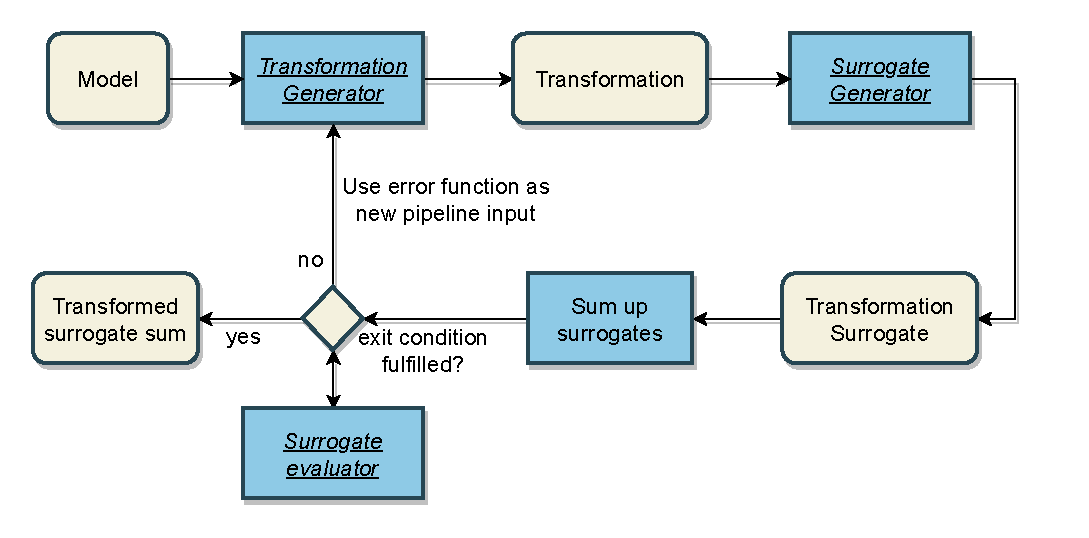
\includegraphics[width=\textwidth]{graphics/TransformationPipeline.pdf}
\vspace{-7.5mm}

\delimit
\vspace{1.5mm}

\begin{description}
\item[Parameters] {~ \begin{itemize}[\indent{}]
\item \texttt{\textbf{exitCondition}}: A predicate indicating whether the pipeline iteration loop should exit. This can make use of a variety of conditions, for example a fixed iteration amount with \texttt{maxIterations($i_{\mathrm{max}}$)} or a relative convergence condition \texttt{relativeConvergence($\eta$)} from \cref{sec:it}.
\item \texttt{\textbf{sampleCount}}: The amount of model observations $n$ used during pipeline execution. These observations are used for a variety of operations and are split into train, validate, and test datasets in each iteration.
\end{itemize}}
\end{description}

\delimit

\caption{Component structure of the transformation pipeline and its associated configuration parameters.}
\label{fig:tp}
\end{figure}
\end{mdframed}
%
The most important component of the transformation pipeline with regards to achieving good approximation results is the transformation generator component (\cref{sec:tg}) as the quality of a single transformation will affect all later iterations.
The generated transformation is fed into a surrogate generator component (\cref{sec:sg}), which will generate the transformed surrogate.
Using the appropriate surrogate generator, any type of surrogate, such as sparse grids or RBFs, can be generated.
The newly generated surrogate is then added to the sum of previously generated surrogates to obtain the new transformed surrogate sum.
At the end of each iteration, we decide whether to exit the pipeline or continue.

\newpage
\section {Transformation generators}
\label{sec:tg}

The transformation generator component has the responsibility of finding a good transformation function to use for a pipeline iteration.
We covered the creation of input transformations extensively in \cref{chap:c4}, and transformation generators are a straightforward implementation of the covered methods.

\subsection {Stream-based transformation generator}
\label{sec:tsg}

We saw previously that we can generate a whole family of transformations for every generated active direction matrix, which is usually accomplished by using different values for the reduced dimensionality $r$, \ie cutting off less or more dimensions.
To apply this concept and to couple it with other components introduced later on, this implementation makes use of so-called transformation stream generators.
A transformation stream generator will generate as much different transformations as it can where the range of generated transformations is usually defined by a minimum and maximum value for $r$.
Every transformation that is generated by a stream generator is first evaluated using a transformation evaluator (\cref{sec:te}) and then compared to the other transformations to choose the best transformation out of all in the end.
The stream-based transformation generator component structure can be seen in \cref{fig:tsg}.

\begin{mdframed}[style=style,frametitle={Transformation generator (stream-based)}]
\begin{figure}[H]
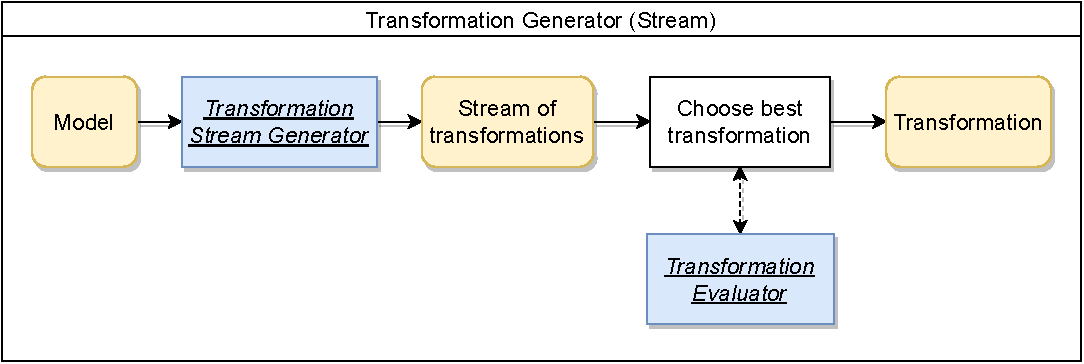
\includegraphics[width=\textwidth]{graphics/TransformationGen_Stream.pdf}
\delimit
\caption{Component structure of a stream-based transformation generator.}
\label{fig:tsg}
\end{figure}
\end{mdframed}
%
Such a design allows us, in theory at least, to parallelize the transformation generation process as we can generate and evaluate all possible transformations in parallel.

\newpage
\subsection{Active Subspace stream generator}

Transformation generation with the active subspaces method, as covered in \cref{sec:as}, is implemented as a transformation stream generator component since there are multiple different cutoff possibilities.
The exact range of the cutoff dimensions can be customized using various parameters, as seen in \cref{fig:astsg}.
However, the general order of active directions from $w_1$ to $w_d$ is still fixed however as it is dictated by the magnitude of the eigenvalues.

\begin{mdframed}[style=style,frametitle={Transformation stream generator (active subspaces)}]
\begin{figure}[H]
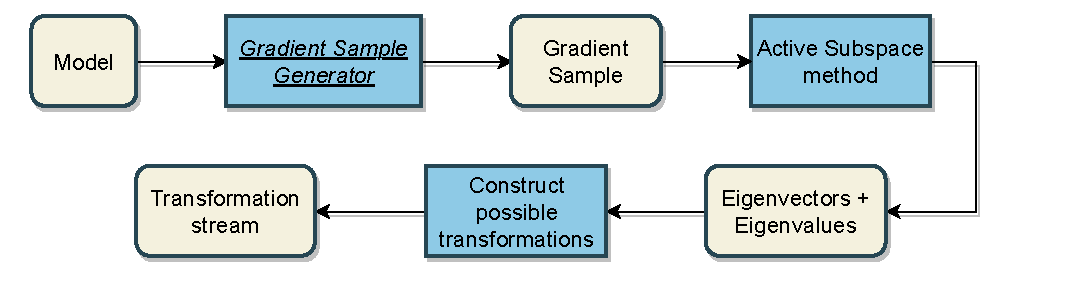
\includegraphics[width=\textwidth]{graphics/TransformationStreamGen_AS.pdf}

\delimit

\begin{description}
\item[Parameters] {~ \begin{itemize}[\indent{}]
\item \texttt{\textbf{maxSampleCount}}: The maximum amount of observations used to create a gradient sample.
\item \texttt{\textbf{minDimensions}}: The minimum amount of used directions, \ie the lower bound for $r$.
\item \texttt{\textbf{maxDimensions}}: The maximum amount of used directions, \ie the upper bound for $r$.
\end{itemize}}
\end{description}
\delimit
\caption{Component structure of an active subspace transformation stream generator and the associated configuration parameters.}
\label{fig:astsg}
\end{figure}
\end{mdframed}
%
The Monte-Carlo based active subspaces method requires gradient samples as inputs.
These are generated by a gradient sample generator component.
If the gradient function of the model function is not known, we can employ various gradient approximation algorithms that we already covered in \cref{sec:as_est}.
Three implementations for gradient approximation are available to choose from as listed in \cref{fig:gg}.

\begin{mdframed}[style=style,frametitle={Gradient sample generators}]
\begin{figure}[H]
\begin{description}
\item[\texttt{\textbf{finiteDifferences($h$)}}:] Gradient samples can be determined using finite differences if the runtime cost of $d$ additional model function evaluations per sample is acceptable.
\item[\texttt{\textbf{randomNeighbours($n'$)}}] Random neighbour approximation using $n'$ random neighbours.
\item[\texttt{\textbf{nearestNeighbours($n', m$)}}] Nearest neighbour approximation that selects the $m$ nearest neighbours out of $n'$ possible ones.
\end{description}
\delimit
\caption{List of available gradient sample generator implementations.}
\label{fig:gg}
\end{figure}
\end{mdframed}

\subsection {Random stream generator}
\label{sec:rtg}

An alternative approach to constructing an active direction transformation is just generating a random one (see \cref{sec:rt}).
This random transformation generator is easy to implement, as shown in \cref{fig:rtsg}, can generate new transformation functions almost instantly, and offers a purely exploratory approach to finding the best transformation.
Random transformations are only viable if many of them are generated consecutively because the chance of finding a good random transformation in one try is very low.
They are therefore mainly used in conjunction with iterative transformation generators (\cref{sec:itg}).

\begin{mdframed}[style=style,frametitle={Transformation stream generator (random)}]
\begin{figure}[H]
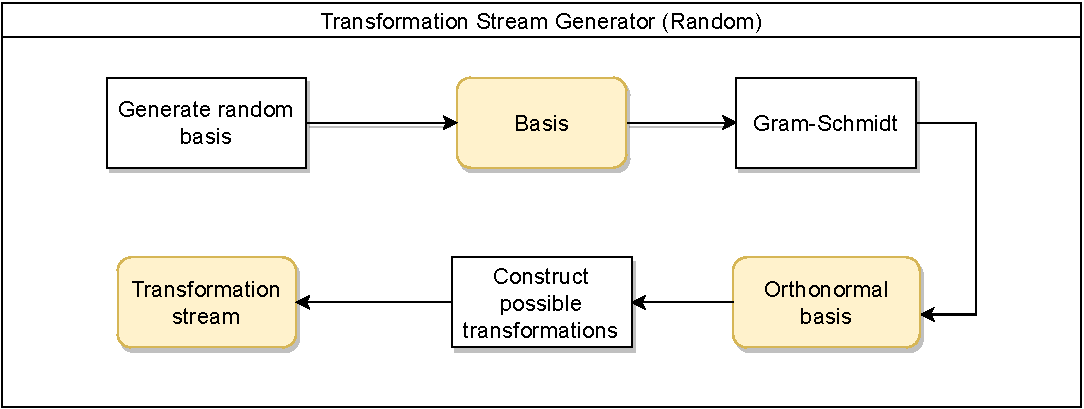
\includegraphics[width=\textwidth]{graphics/TransformationStreamGen_Random.pdf}
\delimit
\begin{description}
\item[Parameters] {~ \begin{itemize}[\indent{}]
\item \texttt{\textbf{minDimensions}}: The minimum amount of used directions, \ie the lower bound for $r$.
\item \texttt{\textbf{maxDimensions}}: The maximum amount of used directions, \ie the upper bound for $r$.
\end{itemize}}
\end{description}
\delimit
\caption{Component structure of an random transformation stream generator and the associated configuration parameters.}
\label{fig:rtsg}
\end{figure}
\end{mdframed}
%
Note that the random active direction matrix generation is also be affected by the curse of dimensionality in the sense that it will become much harder to find a good random transformation in higher dimensionalities because there are many more degrees of freedom for a single active direction vector and also a lot more possible orderings of multiple active direction vectors.
Since the ordering process can be seen as a combination of a set of orthonormal vectors without replacement, the amount of possible combinations given a set of $d$ active directions is $\binom{d}{r} r!$, which increases sharply as $r$ and $d$ grows.

\newpage

\subsection {Iterative transformation generator}
\label{sec:itg}

In some cases, for example when dealing with random transformation generation, it makes sense to introduce an iterative transformation generator component, which can be combined with any other transformation generator component.
A transformation evaluator component (\cref{sec:te}) is responsible for assigning comparable quality ratings to each generated transformation such that the best one can be returned after the iteration limit is reached.
This process is shown in \cref{fig:itg}.

\begin{mdframed}[style=style,frametitle={Transformation generator (iterative)}]
\begin{figure}[H]
	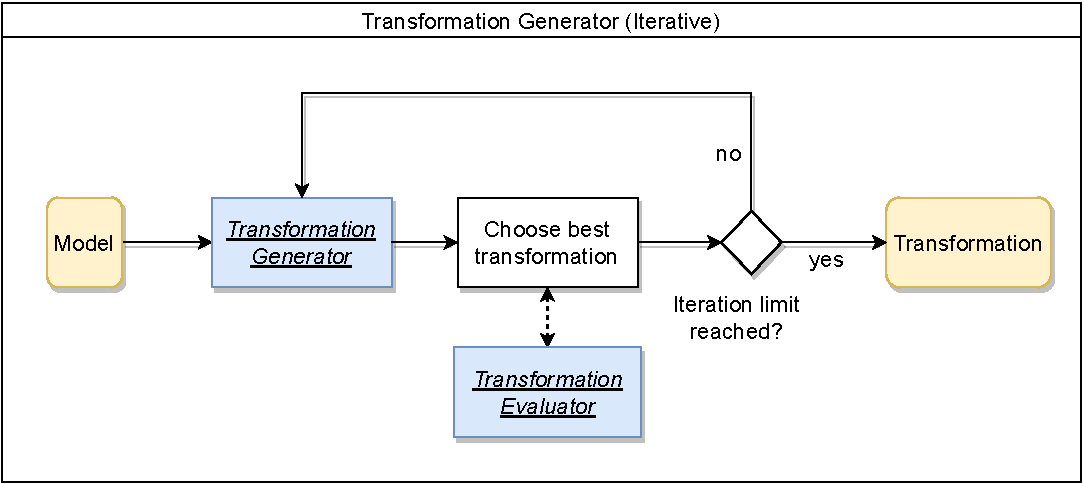
\includegraphics[width=\textwidth]{graphics/TransformationGen_Iterative.pdf}
\delimit

\begin{description}
\item[Parameters] {~ \begin{itemize}[\null]
\item \texttt{\textbf{numIterations}}: The amount of iterations that should be executed.
\end{itemize}}
\end{description}

\delimit
\caption{Component structure of an iterative transformation generator and the associated configuration parameters.}
\label{fig:itg}
\end{figure}
\end{mdframed}
%
Note that this iterative approach is independent from the pipeline iterations, \ie an iterative transformation generator executes all of its iterations during one pipeline step to determine the best transformation that should be used in the current pipeline step.
To achieve fast execution of many iterations, we choose to work on low-fidelity surrogates during the iterations when interacting with transformation evaluator.
This means that the approximation errors used to identify the best transformation do not necessarily come close to the actual high-fidelity approximation errors.

\section {Surrogate generators}
\label{sec:sg}

The last component needed for the pipeline implementation is the surrogate generator, which constructs the function $\hat{f}_t$ for given configuration parameters and transformed input samples,
\begin{equation}
S_t=\left\{\left(t(x_i), f(x_i)\right)\right\}_{i=1}^n \subseteq T \times \mathds{R}.
\end{equation}
The implementation is straightforward and closely matches the construction of sparse grid surrogates in \cref{chap:c4} and of RBF surrogates in \cref{sec:rbf}.

\subsection {Sparse Grid surrogate generator}

Sparse grid generators are implemented using the $\mathrm{SG}^{++}$ library \cite{Pflueger2010}.
The configuration parameters of a sparse grid surrogate generator contains all the usually required inputs like grid type, basis type, several adaptivity properties, and regression parameters.
Instead of passing a fixed level $\ell$ as a parameter, we instead specify how much grid points the surrogate should approximately have and determine the most appropriate level and refinement amounts from there as it varies greatly for different values of $r$.
This guarantees that sparse grids of different dimensionalities all contain an almost equal amount of grid points, which is very useful when performing comparisons.
We are able to come very close to a targeted grid point amount $g$ by performing refinements a certain amount of times on a regular sparse grid of the largest possible level, \ie generating a regular sparse grid with
\begin{equation}
\ell_{\mathrm{max}}=\left\{\abs{X^{\mathrm{s}}_{\ell}} \leq g \mid \ell \in \mathds{N}\right\}
\end{equation}
and padding up the missing amount of grid points using refinements.
Furthermore, for sparse grid regression we similarly express the amount of training samples with the variable \texttt{trainSamplesPerGridPoint} to automatically link the amount of grid points and used training samples together.

\subsection {RBF surrogate generator}

Radial basis function surrogate generation is implemented with the help of ALGLIB \cite{Bochkanov}, a numerical analysis and data processing library that supports fitting RBFs on arbitrary input data.
Compared to sparse grids, RBFs do not have a lot of configuration parameters.
The main parameters are the shape parameter $\epsilon$ and also a regularization factor $\lambda$.
RBF surrogates can be created with the interpolation approach since they can interpolate from arbitrary model observations.

\section {Evaluators}

To judge the quality of transformations and surrogates, we introduce evaluator components.
These take a transformation or surrogate as an input and output a real number that represents their quality and allows for comparisons with others.

\subsection {Surrogate evaluator}
\label{sec:se}

A surrogate evaluator is a simple component that computes the surrogate approximation error by using validation observations and an error metric to compute the Monte-Carlo approximation error of the surrogate, \eg the MSE, RMSE, or NRMSE.
To compute the approximation error, we can either implement a simple train-validate observation split or make use of a more sophisticated cross-validation approach.
Furthermore, this straightforward evaluation can also be customized, for example by adding penalty terms for certain surrogate features, \eg the surrogate dimensionality or regression regularization parameters to steer the transformation pipeline, which relies on these evaluation results, in a certain direction.

\newpage
\subsection {Transformation evaluator}
\label{sec:te}

The role of a transformation evaluator is to take a newly constructed transformation, evaluate its quality, and make it comparable to other transformations.
As discussed in \cref{sec:trans_gen}, evaluating the true quality of a transformation is only really possible by creating a transformed surrogate with it.
We therefore generate a surrogate first and then make use of a surrogate evaluator to return the evaluation result.
This is illustrated in \cref{fig:te}.
While this is a pretty straightforward process, it can still be customized by changing the surrogate construction rules, for example by using a low-fidelity surrogate generator to speed up the evaluation.

\begin{mdframed}[style=style,frametitle={Transformation evaluator (forward looking)}]
\begin{figure}[H]
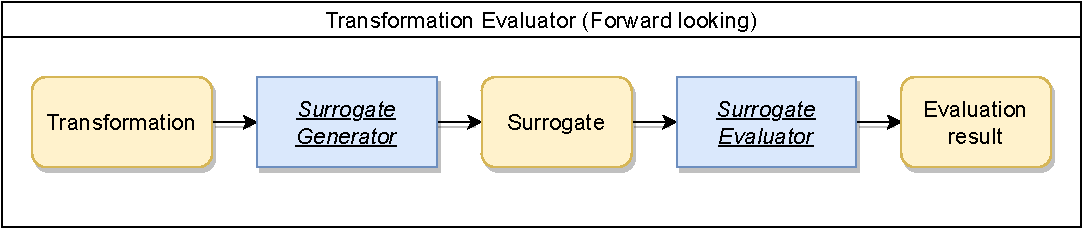
\includegraphics[width=\textwidth]{graphics/TransformationEval.pdf}
\delimit
\caption{Component structure of a forward looking transformation evaluator.}
\label{fig:te}
\end{figure}
\end{mdframed}


\subsection{Observation sample budgeting}

A central aspect of the transformation is pipeline is the handling of observations since they are used in almost every pipeline component.
With the heavy use of the same observations across various stages, special care has to be taken to prevent all kinds of overfitting that can occur.
For example, the generator components and evaluator components should all work on different observations such that no overfitting can possibly take place.

Furthermore, components that only work together, such as the surrogate generator and surrogate evaluator, are internally designed to coordinate their observation use with each other.
For example, a cross validated surrogate evaluator partitions the observation samples multiple times and passes the train partition to the surrogate generator and then evaluates the quality using the associated validate partition.
Therefore, the actual implementation control flow is not as simple as shown in \cref{fig:tpex}.
The observation subset, which is passed down by each component to the next ones, is also randomly shuffled such that partitioning them into train and validation sets is not deterministic when performing multiple pipeline iterations.

In general, the pipeline works fine for any amount of observations as long there is at least a minimum viable amount.
It also does not require any additional function evaluations to work if an appropriate transformation generator is chosen.
This is an advantage compared to any interpolation based approach and makes the transformed surrogate technique very flexible.

\newpage
\section{Example pipeline}

To give an example on how an actual transformation pipeline instance could look like, we will construct a simple one in this section.
As many components are designed to be forward looking, we can think of the transformation pipeline as a collection of different sub-pipelines.
The high-fidelity sub-pipeline is responsible for finding the the best and most expensive possible surrogate that will be returned after each complete pipeline iteration.
It achieves this by usually evaluating the quality of multiple transformations from one family of possible transformations using a look-ahead approach, \ie executing a low-fidelity sub-pipeline that evaluates the transformation quality by effectively performing a whole iteration with low-fidelity surrogates for every possible transformation.
This low-fidelity sub-pipeline has to be quick to execute as it gets executed potentially many times..
The structure of an example pipeline can be seen in \cref{fig:tpex}.

\begin{mdframed}[style=style]
\begin{figure}[H]
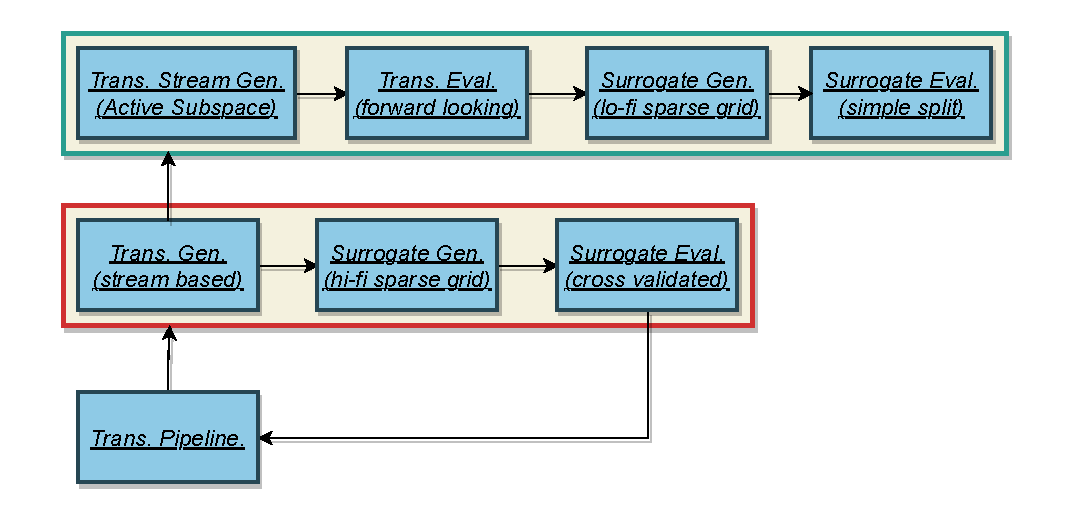
\includegraphics[width=\textwidth]{graphics/PipelineExample.pdf}
\delimit

\captionof{figure}{Structure and control flow of an exemplary transformation pipeline.\\
The \red box represents the high-fidelity sub-pipeline components, and the \green box identifies the low-fidelity sub-pipeline components.}
\label{fig:tpex}
\end{figure}
\end{mdframed}

\chapter{Experiments}
\label{chap:c7}

The construction process for transformed surrogates is realized through the transformation pipeline, which consists out of many different components.
These components interact with each other by exchanging data and are therefore vulnerable to compounding inaccuracies and errors.
In this evaluation chapter, we investigate the qualities and properties of transformation pipeline components in an isolated environment such that we can obtain concrete data for each component that enables us to make use of the best possible pipeline configurations when performing experiments on real-world model functions in the next chapter.
Of course, since not all components can be perfectly isolated, we will settle with best effort approaches that try to be as convincing as possible.
We will first look at the low-dimensional Ishigami function followed by the higher-dimensional wing weight function.

All approximation error results throughout the chapter are computed using a Monte-Carlo NRMSE surrogate evaluator with $10^5$ separate observations.
Furthermore, the sparse grid surrogate generator uses a value of $\texttt{trainSamplesPerGridPoint}=1$ when creating the regression surrogate.
The concrete grid point amount of low-fidelity and high-fidelity surrogates varies and is explicitly mentioned in each section.

\section{Ishigami function}

We start off with the three-dimensional Ishigami function,
\begin{equation}
i(x)=\sin(x_1) + a \sin^2(x_2) + b x_3^4 \sin(x_1), ~~ a = 7, b=0.1,
\end{equation}
%
which has been originally used for uncertainty quantification purposes in \cite{Ishigami1990AnIQ}.
It has also been used to test sensitivity analysis techniques in \cite{Sobol1999}.
To get an idea of the general structure and importance of the inputs, we first apply the active subspace method on this function. It yields the following results:
\begin{mdframed}[style=style]
\begin{figure}[H]
\centering

\bgroup
\def\arraystretch{1.2}%
  \begin{tabular}{ l | c c c}
$i$ & $w_i$ & $\lambda_i$ & $\lambda_i / \sum_{i=1}^d \lambda_i$\\
\hline
$1$ & $(+0.005, ~+0.999, ~+0.007)^T$ & 967.93 & $81.7\%$\\
$2$  & $(+0.540, ~+0.003, ~-0.841)^T$ & 112.20 & $9.5\%$\\
$3$ & $(-0.841, ~+0.008, ~+0.540)^T$ & 104.77 & $8.8\%$\\
\end{tabular}
\egroup
\vspace{0.5em}

\delimit

\captionof{table}{Computed eigenvectors, eigenvalues, and eigenvalue shares of the active subspace matrix for the Ishigami function using the Monte-Carlo method and $10^5$ observations with finite differences.}
\label{tab:ishigami_as}
\end{figure}
\end{mdframed}
%
Based on the values in \cref{tab:ishigami_as}, we can see that the most active direction almost exactly corresponds to second input dimension and is responsible for a big chunk of the average gradient change while the other two directions are less important and are also not axis aligned.
These two less active directions are however not negligible beucase their combined eigenvalue share still is $18.3\%$.

\subsection{Dimensionality preserving transformations}

While the main focus of this thesis lies on reducing transformations with $r < d$, we still take a short look at the quality of simple dimensionality preserving transformations with $r=d$, which are effectively only changing the orientation of the function input parameters.
For the orientation change, we use all computed active directions from \cref{tab:ishigami_as}.
In other words, we apply the active direction transformation $t_{W_3}$ (see \cref{sec:ruh}) on the inputs.
As discussed in \cref{sec:ms}, with a few small modifications concerning model function evaluations outside of $\Omega$, we can also apply the interpolation method to construct a transformed sparse grid surrogate.
Compared the non transformed interpolation approach, the approximation error should be improved by the more optimal orientation of inputs.
On the other side, the unused parts of surrogate space (see \cref{sec:tis}) effectively reduce the grid point resolution of the sparse grid surrogate and may make some grid points obsolete.
Furthermore, the necessary model function evaluations outside of $\Omega$ might worsen the approximation quality if they deviate sharply from function values inside $\Omega$ and might create steep value differences at the boundaries of $T$.
In this section, we are interested in answering the following basic questions:
\begin{enumerate}
\item How does the approximation error compare when applying an orientation changing transformation with $r=d$?
\item How big is the approximation error difference between interpolation and regression surrogates?
\item How is the approximation error affected when transformations and regression are used together?
\item How much difference is there between regular sparse grids and regular sparse boundary grids?
\end{enumerate}
\Cref{fig:ishigami_errors} shows the first comparison results of untransformed and transformed sparse grid surrogates created using interpolation and regression.
\begin{mdframed}[style=style]
\vspace{-3mm}
\begin{figure}[H]
\centering
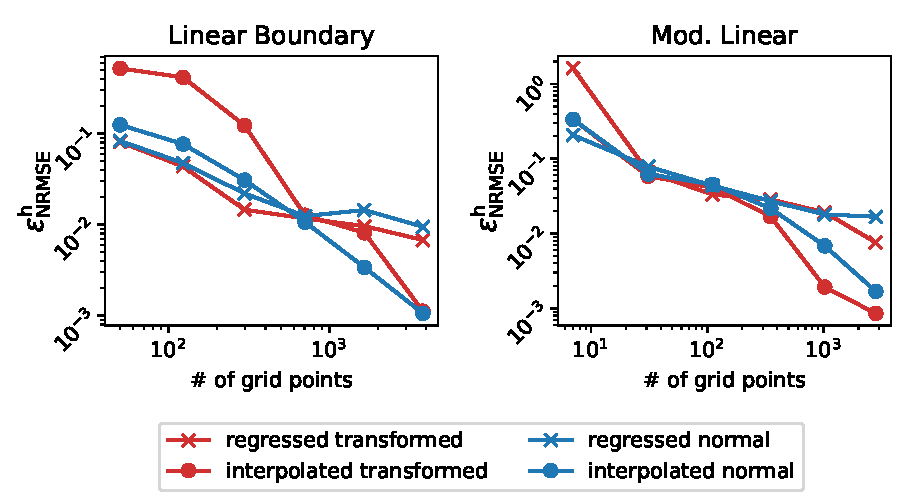
\includegraphics[width=0.9\textwidth]{graphics/ishigami_orientation}\vspace{-4mm}
\delimit
\captionof{figure}{Approximation errors of transformed and untransformed sparse grid surrogates with $\ell \in \{2, \dots, 7\}$ for the Ishigami function using boundary hat basis functions and modified hat basis functions. The transformations were constructed using the active directions from \cref{tab:ishigami_as} and only one pipeline iteration was performed.}
\label{fig:ishigami_errors}
\end{figure}
\end{mdframed}
%
As we can see in \cref{fig:ishigami_errors}, the pure orientation change does not lead to better interpolation results.
In this concrete example, the penalty of the unused transformation space $U$ evens out the gains from a more optimal orientation for sparse grid surrogates.
As we do not perform a dimensionality reduction, even if it would be feasible, this results in a constructed surrogate space that covers a lot more than the required transformation space.
In this case, the unused surrogate space share is $\tilde{u}_t=0.44$, which means that $T$ only makes up $56\%$ of the surrogate space $S$.
This effectively lowers the grid point resolution and results in some grid points being unused.
Furthermore, the introduced regression penalty factor is approximately $10^1$ compared to the interpolation method.

There are also no significant quality differences when using modified hat basis functions instead of a hat basis with boundaries.
Therefore, we will only use the modified hat basis for the Ishigami function later in this evaluation section.

Based on these results, we can conclude that, even though there is no improvement with this method, there is also no significant downside even as $\tilde{u}$ is relatively large and regression is employed.
This can be seen as a positive insight because it means that having a lot of unused space, which can not be avoided when using active direction transformations, approximately cancels out with the orientation improvements.
Moreover, the additional use of regression only results in a slight increase of the approximation error.
As the transformation process focuses on reducing transformations that have to deal with unused space and can only use regression, this means that the individual transformed sparse grid surrogates do not become worse just through the orientation change but allow for a much more flexible dimensionality reduction process.
Therefore, dimensionality reducing transformations seem to have a much bigger potential.

\subsection{Dimensionality reducing transformations}

Next, we look at dimensionality reducing transformations with $r < d$.
Note that for this low-dimensional model function, there is no real need to perform a dimensionality reduction as the curse of dimensionality does not really affect sparse grid surrogates for $d=3$.
We can therefore not expect to see any gain from applying a transformation with $r < d$.
Even though reducing transformations should not be competitive for the Ishigami function, we are still interested in answering some basic questions:
\begin{enumerate}
\item By how much does dimensionality reduction increase the approximation error?
\item How much do the increased approximation errors correlate with the computed active subspace eigenvalues?
\end{enumerate}
%
Based on the active subspace information from \cref{tab:ishigami_as}, a one-dimensional reduction by cutting off the eigenvectors $v_2$ and $v_3$ looks feasible because the first active direction covers the majority of the eigenvalue share.
However, as already discussed in \cref{sec:asl}, the active subspace method can be biased and may not produce suitable active directions and eigenvalues.
Therefore, the primarily used pipeline component uses a look ahead approach to evaluate the suitability of the computed active directions and corresponding eigenvalues instead of relying solely on the active subspaces results.

To better investigate the active subspace properties, we first generate transformations for $r=1$ and $r=2$.
Since these are dimensionality reducing transformations, we can only create regression surrogates.
Then we compare them to regression and interpolation surrogates with $r=3$ to obtain the added approximation error.

\newpage
\begin{mdframed}[style=style]
\begin{figure}[H]
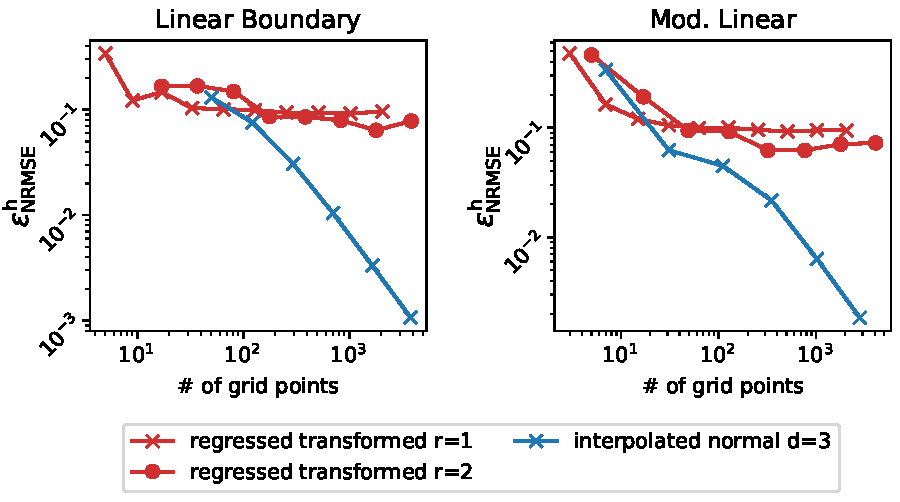
\includegraphics[width=\textwidth]{graphics/ishigami_red}\vspace{-2mm}
\delimit
\captionof{figure}{Approximation errors of various transformed sparse grid surrogates with $\ell \in \{2, \dots, 7\}$ for the Ishigami function using boundary hat basis functions and modified hat basis functions. The transformations were constructed using the active directions from \cref{tab:ishigami_as} and only one pipeline iteration was performed.
The interpolation result is included as a reference.}
\label{fig:ishigami_red}
\end{figure}
\end{mdframed}
%
As we can see in \cref{fig:ishigami_red}, the dimensionality reducing transformations lead to, as expected, way worse results and do not provide competitive surrogates.
We see that the approximation error for the reduced surrogates reaches a convergent state very fast and an increase in grid points does not improve the surrogate quality.
Furthermore, the actual approximation error of the reduced surrogates does not correlate with the active subspace eigenvalues.
Even though the eigenvalue share of the first two eigenvectors is around $90\%$, the loss of the approximation quality when cutting of the most inactive eigenvector in the $r=2$ case is already very large.

\subsection{Multiple iterations}

After we looked at the results of a mostly static pipeline in the sense that $r$ was fixed, we now continue to look at a more dynamic pipeline approach.
The goal here is to dynamically choose a suitable reduced dimensionality value $r_i$ for each iteration such that we can obtain better results than with a purely static pipeline.
By specifying how many grid points should be added in each iteration, we can easily implement a dynamic pipeline that determines the best $r_i$ by looking ahead and then creates a sparse grid surrogate with the given amount of grid points.
The amount of grid points added per iteration can be customized with the goal of finding the best amount.
We are interested in answering the following questions:
\begin{enumerate}
\item Do multiple iterations deliver better results than a single one?
\item Are there differences between the amount of grid points added per iteration?
\end{enumerate}
Results for various grid point amounts are shown in \cref{fig:ishigami_dyn}, which showcases dynamic pipeline results that use a different amount of grid points per iteration (gp/it).

\begin{mdframed}[style=style]
\begin{figure}[H]
\vspace{-2mm}
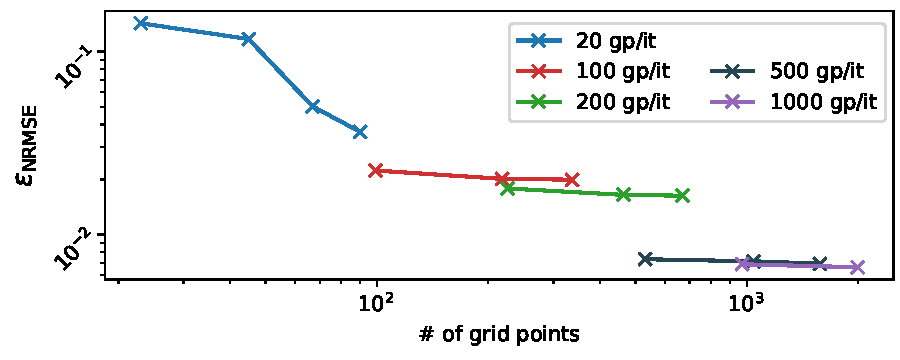
\includegraphics[width=\textwidth]{graphics/ishigami_dynamic}\vspace{-4mm}
\delimit
\captionof{figure}{Approximation errors of various transformed surrogate sum approximations for the Ishigami function created using a dynamic pipeline.\\
In contrast to previous figures, every marker of a graph in \cref{fig:ww_dyn} now represents the result of a new iteration with the approximation error of the new surrogate sum and the grid point amount of all surrogate sum elements combined.}
\label{fig:ishigami_dyn}
\end{figure}
\end{mdframed}
%
As we are able to see, the gains from using multiple iterations are, except in the 20 gp/it case, nonexistent.
This might be explained by the fact that reducing transformations are very ineffective at approximating the function and therefore force the iterative algorithm to always construct three-dimensional surrogates as they still provide the best approximation quality.
We therefore wait for the high-dimensional function evaluation later in this chapter to judge the true potential of the iterative algorithm because it can not deliver any gains for low-dimensional model functions like this.

\subsection{Random transformations}

To verify the quality of the active subspace method compared to a true optimal active direction transformation, which we can't necessarily construct deterministically using active subspaces, one approach are random active direction transformations (see \cref{sec:rt}).
This generation method is not affected by any potential biases or compounding gradient approximation errors like the active subspace method is.
To effectively make use of this strategy, it is vital that we can quickly generate, evaluate, and discard many random transformations, as more generated transformations will allow us to get closer to the potential optimal transformation.
As the mainly used transformation evaluator component is forward looking, \ie generating an actual transformed surrogate, we have to employ very low-fidelity components to achieve a large amount of runs.
We are interested in answering the following questions:
\begin{enumerate}
\item How do the best found random transformations compare to active subspaces?
\item What does the approximation error distribution of the randomly generated transformations look like?
\item Are random active direction transformations a viable alternative for constructing transformations?
\end{enumerate}
%
Once the algorithm has determined the random transformation with the lowest error based on the low-fidelity surrogates, we construct an actual high-fidelity surrogate and calculate the error again.
The low-fidelity transformation errors are visualized using histograms and while the errors do not come close to the actual high-fidelity errors, the distribution of low-fidelity errors can provide valuable insights into the actual approximation error distribution since the low-fidelity surrogates are chosen to be comparatively representative.

As we will make use of low-fidelity and high-fidelity simulations, we will distinguish the resulting errors by denoting them by $\varepsilon^\mathrm{l}_{\mathrm{NRMSE}}$ and $\varepsilon^\mathrm{h}_{\mathrm{NRMSE}}$, respectively.
For the Ishigami function in the low-fidelity case, we use a sparse grid surrogate generator with modified hat basis functions, and 250 grid points..
In the high-fidelity case, we increase the grid point amount to $10^3$.
We only perform one pipeline iteration as we already saw that additional iterations do not considerably improve the approximation.

\begin{mdframed}[style=style]
\begin{figure}[H]
\begin{subfigure}{.5\textwidth}
  \centering
   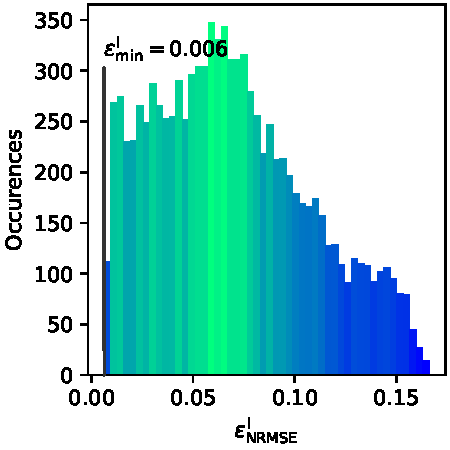
\includegraphics[width=0.95\linewidth]{graphics/ishigami_hist_3_inter}
  \subcaption{Interpolated transformed sparse grid surrogates with $r=3$. The resulting high-fidelity error is $\varepsilon^\mathrm{h}_{\mathrm{min}}=0.0007$.}
\vspace{3mm}
  \label{fig:ishigami_hist_3_inter}
\end{subfigure}%
\begin{subfigure}[H]{.5\textwidth}
  \centering
   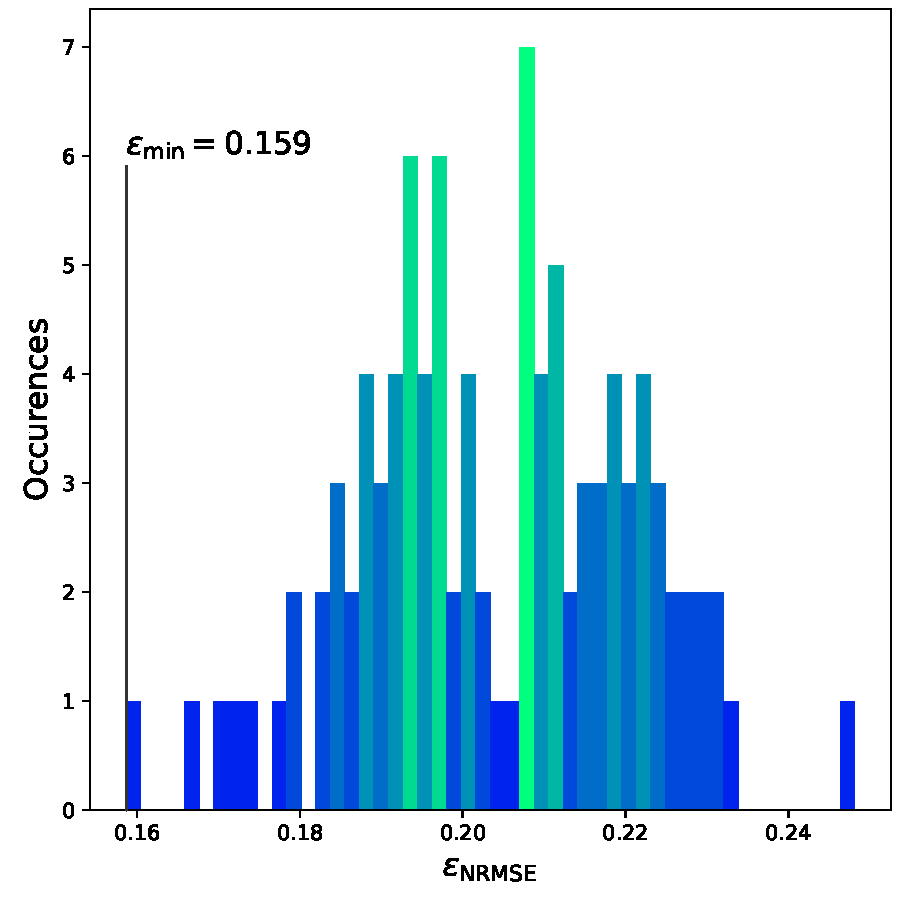
\includegraphics[width=0.95\linewidth]{graphics/ishigami_hist_3}
  \subcaption{Regressed transformed sparse grid surrogates with $r=3$. The resulting high-fidelity error is $\varepsilon^\mathrm{h}_{\mathrm{min}}=0.031$.}
\vspace{3mm}
  \label{fig:ishigami_hist_3}
\end{subfigure}
\delimit
  \caption{Histogram of low-fidelity approximation errors for $10^4$ randomly generated transformations and the associated best possible high-fidelity error.}
\label{fig:ishigami_hists_pres}
\end{figure}
\end{mdframed}
%
\Cref{fig:ishigami_hists_pres} shows the approximation error distribution of interpolation and regression surrogates for $r=3$.
Comparing the high-fidelity results with $10^3$ grid points to the previous active subspace transformation results in \cref{fig:ishigami_red}, we see that random transformations can deliver competitive results.
We see that the distribution has a broad center of mass and almost no real tails, which makes it easier to find good transformations.

\newpage
\begin{mdframed}[style=style]
\begin{figure}[H]
\begin{subfigure}{.5\textwidth}
  \centering
   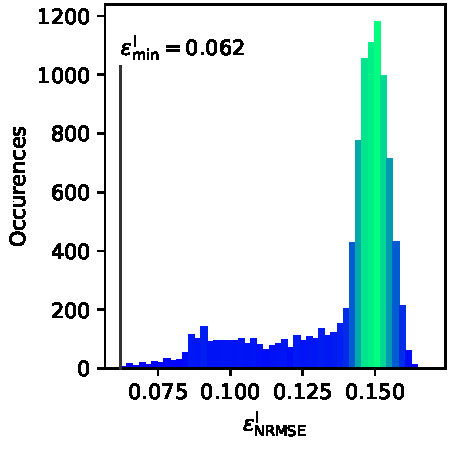
\includegraphics[width=0.95\linewidth]{graphics/ishigami_hist_2}
  \subcaption{Regressed transformed sparse grid surrogates with $r=2$. The resulting high-fidelity error is $\varepsilon^\mathrm{h}_{\mathrm{min}}=0.05$.}
\vspace{3mm}
\label{fig:ishigami_hist_2}
\end{subfigure}%
\begin{subfigure}{.5\textwidth}
  \centering
   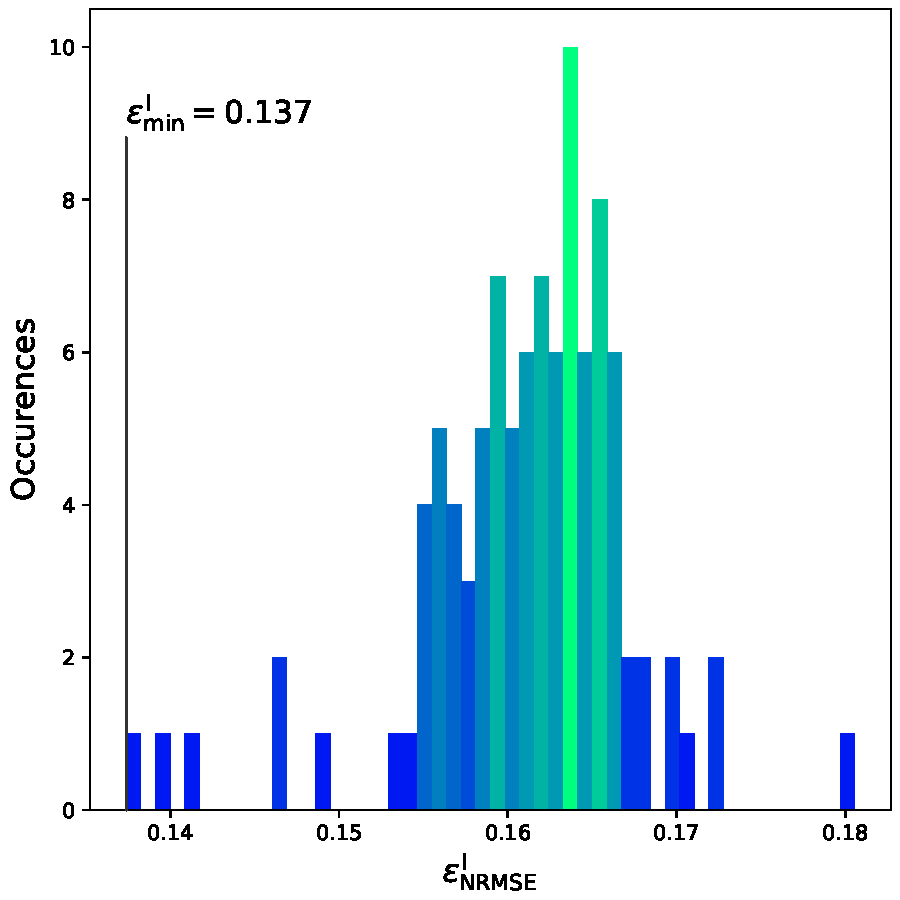
\includegraphics[width=0.95\linewidth]{graphics/ishigami_hist_1}
  \subcaption{Regressed transformed sparse grid surrogates with $r=1$. The resulting high-fidelity error is $\varepsilon^\mathrm{h}_{\mathrm{min}}=0.09$.}
\vspace{3mm}
\label{fig:ishigami_hist_1}
\end{subfigure}
\delimit
  \caption{Histogram of low-fidelity approximation errors for $10^4$ randomly generated transformations and the associated best possible high-fidelity error.}
\label{fig:ishigami_hists_red}
\end{figure}
\end{mdframed}
%
In \cref{fig:ishigami_hists_red} with $r=1$ and $r=2$, the distribution shape changes drastically to a distribution with a high peak, very long tails and a negative skew.
As a result, it requires more generation runs to obtain a good transformation because the probability of finding one far too the left of the peak is low.
However, compared to the results in \cref{fig:ishigami_red}, the best found transformation still delivers similar results to active subspaces.

In conclusion, random transformation generation proves to be a valuable alternative to active subspaces, at least for this example function and enough runs, as it comes close to the active subspace transformations.
However, for higher dimensional functions, the required amount of random generation iterations to find an acceptable transformation is expected grow very fast, as more dimensions will mean more possible directions and also orders of directions.
Therefore, we expect the active subspace method to scale better with higher dimensions as it only requires exactly one run and an order of directions is implicitly given.

\newpage
\section{Wing weight function}

Now that we investigated several important pipeline components with regards to their properties when being applied to a low-dimensional model function, we compare the results to a case study that involves a high-dimensional model function to look out for properties that can't be generalized from one low-dimensional case study.
The model function covered in this section is the wing weight function \cite{Forrester2008},
\begin{equation}
w=0.036 \, S_\mathrm{w}^{0.758} \, W_\mathrm{fw}^{0.0035} \left(\frac{A}{\cos^2(\Lambda)}\right)^{0.6} q^{0.006} \lambda^{0.04} \left( \frac{100 t_\mathrm{c}}{\cos(\Lambda)} \right)^{-0.3} (N_\mathrm{z} W_\mathrm{dg})^{0.49} + S_\mathrm{w} W_\mathrm{p},
\end{equation}
which models the weight of a wing for a light aircraft based on ten input parameters that are defined in \cref{tab:ww_params}.
It has already been studied in the context of sensitivity analysis in \cite{Moon2012}.
\begin{mdframed}[style=style]
\begin{figure}[H]
\vspace{-2mm}
\centering
\bgroup
\def\arraystretch{1.2}%
  \begin{tabular}{ l l l l}
Variable & Description & Distribution\\
\hline
$S_{\mathrm{w}}$ & wing area (ft$^2$) & $\mathcal{U}(150,\, 200)$\\
$W_{\mathrm{fw}}$ & weight of fuel in the wing (lb) & $\mathcal{U}(220,\, 300)$\\
$A$ & aspect ratio & $\mathcal{U}(6,\, 10)$\\
$\Lambda$ & quarter-chord sweep (degrees) & $\mathcal{U}(-10 ,\,  10)$\\
$q$ & dynamic pressure at cruise (lb/ft$^2$) & $\mathcal{U}(16,\, 45)$\\
$\lambda$ & taper ratio & $\mathcal{U}(0.5, \, 1)$\\
$t_\mathrm{c}$ & aerofoil thickness to chord ratio & $\mathcal{U}(0.08\, 0.18)$\\
$N_\mathrm{z}$ & ultimate load factor & $\mathcal{U}(2.5\, 6)$\\
$W_\mathrm{dg}$ & flight design gross weight (lb)& $\mathcal{U}(1700\, 2500)$\\
$W_\mathrm{p}$ & paint weight (lb/ft$^2$) & $\mathcal{U}(0.025,\, 0.08)$\\
\end{tabular}
\egroup\\
\vspace{0.5em}
\delimit
\captionof{table}{Input parameters of the wing weight model function.}
\label{tab:ww_params}
\end{figure}
\end{mdframed}
%
To get an idea of the general structure and importance of the inputs, we apply the active subspaces method on this function as well, which yields the results of \cref{tab:ww_as}.
\begin{mdframed}[style=style]
\begin{figure}[H]
\vspace{-2mm}
\centering
\bgroup
\def\arraystretch{1.2}%
  \begin{tabular}{ l | c c c}
$i$ & $\lambda_i$ & $\lambda_i / \sum_{i=1}^d \lambda_i$\\
\hline
$1$  & 28318.959 & $97.1\%$\\
$2$   & 478.48 & $1.6\%$\\
$3$  & 200.70 & $0.7\%$\\
$4 \dots 10$  & < 71.0 & $< 0.02\%$\\
\end{tabular}
\egroup
\vspace{0.5em}

\delimit

\captionof{table}{Computed eigenvalues and eigenvalue shares of the active subspace matrix for the wing weight function using the Monte-Carlo method and $10^5$ samples with finite differences.}
\label{tab:ww_as}
\end{figure}
\end{mdframed}
%
Based on the values in \cref{tab:ww_as}, we can see that there exists one dominant active direction that takes up the majority of the eigenvalue share and that there are two less important active directions as well.
The seven other directions only make up a very small share of the total eigenvalue sum.

\noindent However, as we learned for the Ishigami function, these eigenvalues should only be used as rough indicators and not as reliable sources about the suitability for using transformed sparse grids.

\subsection{Static pipeline}

To start off, we first investigate the general quality of active direction transformations with multiple iterations and fixed $r$ to get an idea of the model function properties with regards to its approximate compounded intrinsic dimensionality.
To achieve this, we use the directions from \cref{tab:ww_as} and employ the relative convergence criterion with $\eta=0$, \ie we perform iterations until the approximation error does not improve anymore.
The results can be seen in \cref{fig:wwf}.

\begin{mdframed}[style=style]
\begin{figure}[H]
\vspace{-2mm}
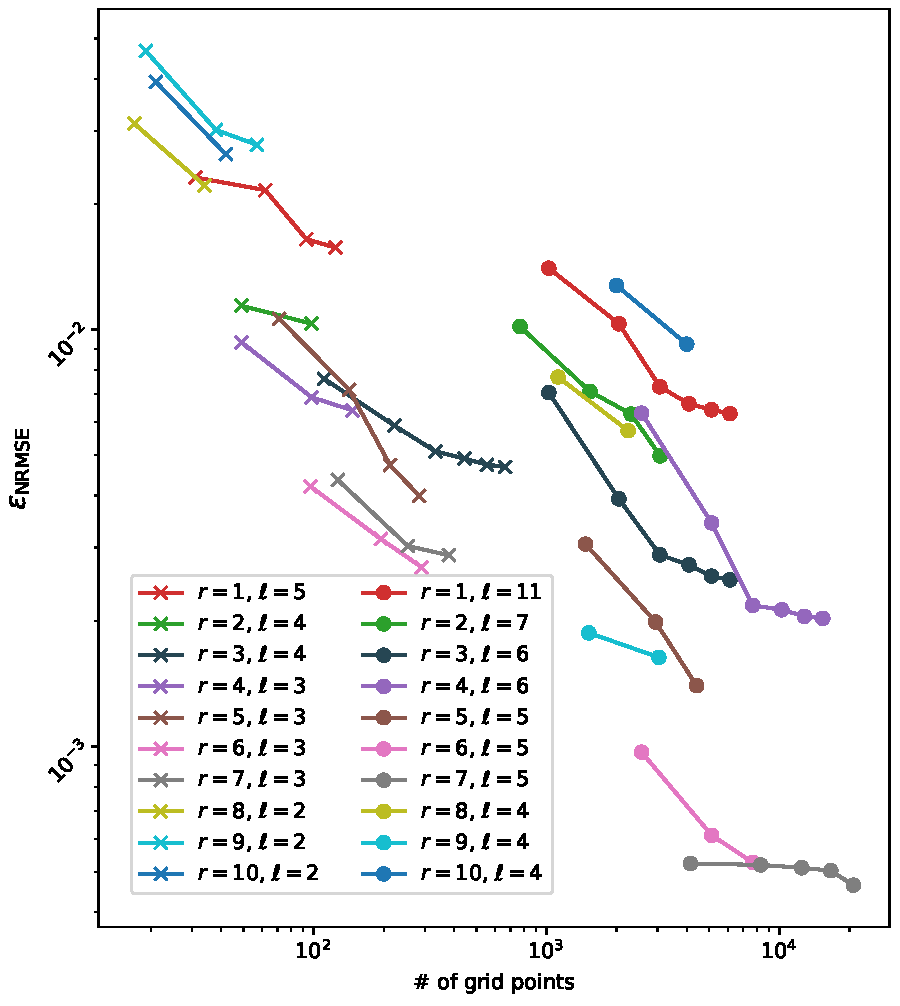
\includegraphics[width=0.97\textwidth]{graphics/wingweight_fixed}\vspace{-4mm}
\delimit
\captionof{figure}{Approximation errors of various transformed surrogate sum approximations with fixed values of $r$ for the wing weight function.}
\label{fig:wwf}
\end{figure}
\end{mdframed}
%
Every marker of a graph in \cref{fig:wwf} represents the result of a new iteration with the approximation error of the new surrogate sum and the grid point amount of all surrogate sum elements combined.
In the left half, we see surrogate sum approximations using a coarse level and in the right half we see the fine level equivalents.
The range between coarse and fine level surrogate sums for the same reduced dimensionality $r$ gives insight into what part of the approximation error is based on the compounded intrinsic dimensionality of the model function and what part is based on the surrogate fidelities itself.
For example, we see that for $r=1, \dots, 4$, the approximation error improvement from low-level to high-level surrogates is relatively small compared to higher values of $r$.
This means that the main limiting factor in these cases is that the model function can not be approximated well with such low-dimensional surrogates.
For $r > 4$, we see bigger improvement gaps when going from low levels to higher levels, which means that there is  more potential approximation quality for higher-dimensional surrogates.

Moreover, we see that multiple iterations do improve the approximation, in contrast to the Ishigami function.
The majority of approximation improvements can be achieved within the first three pipeline iterations as most error graphs converge after the third iteration.
As we make use of static pipeline iterations only and therefore do not have the freedom to optimally choose the best reduced dimensionality in each iteration, we also might limit the effectiveness of multiple iterations.

Another interesting trend that can be observed is the behaviour of the approximation errors as $r$ grows.
The general approximation quality improves from $r=1$ to $r=7$ but hits a point at which the trend reverses and then worsens from $r=7$ to $r=10$.
This can be explained by the general tradeoff between grid point resolution and dimensionality.
As higher-dimensional grids effectively have to spend less grid points for each dimension when keeping the amount of grid points constant, this results in a tradeoff between grid points spent per dimension and reduced dimensionality.
This optimal tradeoff point is hit at $r=7$ in this case.

All in all, we can conclude that higher reduced dimensionalities up to $r=7$ provide the best approximation error tradeoff when comparing the results for an equal amount of grid points
This does not correlate at all with the active subspace results from \cref{tab:ww_as} and reinforces the evidence that we should not rely on the active subspace eigenvalues.
The greater difference between low-fidelity and high-fidelity surrogates for larger values of $r$ means that applying transformation generators that require a lot of low-fidelity surrogates, such as the random active direction generators, will take up more runtime as the amount of grid points for low-fidelity surrogates has to be increased to produce representative surrogates.

\subsection{Dynamic pipeline}

After we looked at the results of a mostly static pipeline in the sense that $r$ was fixed, we now continue to look at a more dynamic pipeline approach.
The goal is to dynamically choose a suitable reduced dimensionality $r_i$ for each iteration such that we can obtain better results than with a static pipeline.
By specifying how many grid points should be added in each iteration, we can easily implement a dynamic pipeline that determines the best $r_i$ by looking ahead and then creates a sparse grid surrogate with the given amount of grid points.
The targeted grid point amount can always be reached by performing refinements a certain amount of times.
We differentiate the dynamic pipeline results by the spent amount of grid points per iteration (gp / it).

\newpage
\begin{mdframed}[style=style]
\begin{figure}[H]
\vspace{-2mm}
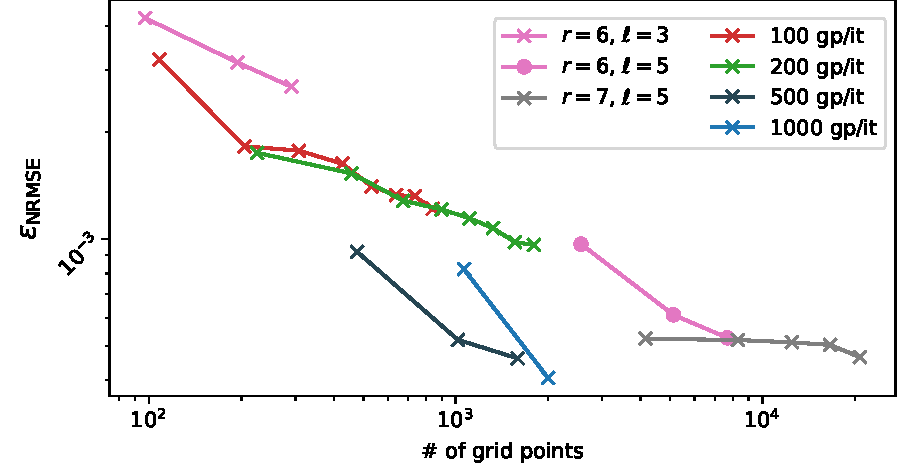
\includegraphics[width=\textwidth]{graphics/ww_dynamic}\vspace{-4mm}
\delimit
\captionof{figure}{Approximation errors of various transformed surrogate sum approximations for the wing weight function created using a dynamic pipeline.
The best results from the static pipeline are also included for reference.}
\label{fig:ww_dyn}
\end{figure}
\end{mdframed}
%
\Cref{fig:ww_dyn} shows that by utilizing a more flexible dynamic pipeline, we can improve the approximation quality a little bit compared to a purely static pipeline.
Furthermore, we also observe that there are differences in the approximation quality between the different amount of grid points spent per iteration as a pipeline with 500 gp/it delivers better results than one with 100 gp/it and 200 gp/it.
Overall, when using the right amount of grid points per iteration, we are able to obtain some improvements.
This is in contrast to the Ishigami function where multiple iterations did not improve the approximation at all.
Therefore, when we have more possible values of $r$ to choose from and when almost all values of $r$ result in somewhat acceptable approximations, the dynamic pipeline approach becomes the better option.

\subsection{Active subspace approximations}

Another central aspect of the transformation pipeline is the quality of the generated transformations for any given value of $r$.
In cases the transformation is constructed using the active subspace method, we are interested in the quality differences between the available active subspace approximation methods (see \cref{sec:as_est}) and want to ideally make use of the neighbour approximation methods because they don't require known gradients and no additional model function evaluations.
We are interested in answering the following questions:
\begin{enumerate}
\item How much do approximated active subspaces differ from the true active subspaces?
\item Do the active subspace differences actually manifest themselves in the approximation error?
\item Which active subspace approximation method performs the best?
\end{enumerate}
\newpage
\noindent
To judge the quality of approximated gradients, we first have to define an error metric for them:
\begin{definition}[Gradient approximation error]
Let $S=\{(x_i, f(x_i)\}_{i=1}^n$ be a set of observations, and let $\widetilde{\nabla} f(x_i)$ be the approximated gradient for each observation point $x_i$. We then define
\begin{equation}
\varepsilon_{\mathrm{grad}}(S) \coloneqq \frac{1}{n} \sum_{i=1}^n \frac{\|{\widetilde{\nabla} f(x_i) - \nabla f(x_i)}\|_2}{{\| \nabla f(x_i) \|}_2}
\label{eq:e_grad}
\end{equation}
as the gradient approximation error of the observation set.
\end{definition}
%
In the context of active subspaces, the approximation error of the gradients is not the relevant metric to evaluate a gradient approximation method.
Instead, the primary focus should be the resulting surrogate approximation error, as it is the only metric that matters in the end.
Even though the active subspaces computation is based entirely on the average outer product of the gradients, there is not necessarily a strong link between $\varepsilon_{\text{grad}}$ and the quality of the resulting active subspace.
While the individual approximated gradients approximated can be far off, the average of the outer products of the gradients can still come close to the real one if the general trend of the gradients is still be reflected in the approximated gradients.
Therefore, inaccuracies of single gradients can be averaged out, but systematic biases of the gradients will influence the approximated active subspace.
The end result doesn't necessarily have to be bad however, as even the true active subspaces might not result in an optimal transformation.

At first glance, using some sort of approximated active subspace deviation looks like a good metric to evaluate approximated active subspaces.
This would entail calculating some matrix norm of the approximation error compared to the true active subspace, that is to calculate $\| W - W^\ast \|$.
However, this error calculation is not suitable for cases in which $\lambda_i \approx 0$, since the corresponding eigenvectors can vary greatly in that case.
Also, if two eigenvalues $\lambda_i, \lambda_j$ are similar in magnitude, the order of eigenvectors might switch arbitrarily and result in a huge matrix norm value.
An error calculation of this type would therefore be potentially very unstable and not suitable.
We therefore settle with the surrogate look ahead approximation error.

\begin{mdframed}[style=style]
\begin{figure}[H]
	\includegraphics[width=\textwidth]{graphics/ww_as_grad_errors}
\delimit
	\caption{Gradient approximation errors of various gradient approximation methods averaged over 10 separate runs.}
	\label{fig:ww_as_grad}
\end{figure}
\end{mdframed}
%
As seen in \cref{fig:ww_as_grad}, the finite differences approximation error converges towards zero as the spacing $h$ goes down, which is to be expected.
Furthermore, both neighbour methods do deliver approximately the same results with regards to $\varepsilon_{\mathrm{grad}}$.
Their gradient errors all lie in a range that is similar to the finite differences approximation with a very big step size of $h=5$, which at first glance makes them look not suitable.
Different configuration parameters for the neighbour-based methods also seem to only improve the gradient approximation error by a small amount.

\begin{mdframed}[style=style]
\begin{figure}[H]
\begin{subfigure}{.5\textwidth}
  \centering
   \includegraphics[width=\linewidth]{graphics/ww_as_10}
	\caption{Surrogates with $r=10$.}
	\label{fig:ww_as_3_inter}
\end{subfigure}
\begin{subfigure}{.5\textwidth}
  \centering
   \includegraphics[width=\linewidth]{graphics/ww_as_7}
	\caption{Surrogates with $r=7$.}
	\label{fig:ww_as_3}
\end{subfigure}\vspace{4mm}
\begin{subfigure}{.5\textwidth}
  \centering
   \includegraphics[width=\linewidth]{graphics/ww_as_4}
	\caption{Surrogates with $r=4$.}
	\label{fig:ww_as_2}
\end{subfigure}
\begin{subfigure}{.5\textwidth}
  \centering
   \includegraphics[width=\linewidth]{graphics/ww_as_1}
	\caption{Surrogates with $r=1$.}
	\label{fig:ww_as_1}
\end{subfigure}\vspace{4mm}
\delimit
	\caption{Surrogate look ahead errors for select values of $r$ using active direction transformations, which were created by using various gradient approximation methods, averaged over 10 separate runs.
	The sparse grid surrogates were created using $10^3$ grid points and modified hat basis functions.}
	\label{fig:ww_as}
\end{figure}
\end{mdframed}
%
\Cref{fig:ww_as} shows the actual performance of the different methods by using the look ahead error.
It can be observed that the gradient approximation quality from \cref{fig:ww_as_grad} does not exactly correlate with the constructed surrogate quality.
While the finite differences method with $h=0.01$ has the best error $\varepsilon_{\mathrm{grad}}$ by far, the constructed surrogate does not perform better than basically the other finite differences methods and also some of the nearest neighbour methods.
The random neighbour method lags a little bit behind in terms of the gradient errors and also surrogate errors in some cases but is still in a comparable range to the other methods.
Furthermore, the nearest neighbour method does deliver far better results than the random neighbour method as it shows a similar quality as the finite differences approximation with smaller step sizes in many cases when $m$ is chosen correctly.

Especially important here are the results for $r=7$ as we have seen that the best approximation errors are achieved for that reduced dimensionality.
Overall, the finite differences method performs the best, followed by the nearest neighbour method with $m=100$.
The random neighbour method performs the worst in almost all cases.
These results are good news as they indicate that the nearest neighbour approximation method, which is way cheaper with regards to required function evaluations, can deliver almost the same results as more expensive methods when the configuration parameters are chosen right.


\subsection{Random active directions}

Similar to the first model function, we also try to find good active directions randomly as well.
This time however, the results should be way worse because finding good active directions in ten dimensions is more difficult.
We saw in the last sections that the wing weight function can already be approximated pretty well with only one transformed surrogate and further iterations do not massively increase the approximation quality.
Therefore, we can already assess whether random active directions are potentially viable by only performing one pipeline iteration.
\Cref{fig:ww_hist_all} shows the low-fidelity approximation error distribution for random active direction generators and the high-fidelity approximation error of the best transformation out of all after one iteration.

When looking at the progression from lower dimensionalities to higher dimensionalities, we see that the distribution shape changes from having long tails and a negative skew to a more balanced bell shape, which makes finding a good transformation located on the left tail harder for higher dimensionalities.
Histograms for $r > 6$ are omitted as they behave very similar with regards to their shape and also approximation errors compared to the histogram for $r=6$.

Moreover, we see that the low-fidelity and high-fidelity errors of the best one-dimensional generation result are better than the best ones for $r=2, \dots, 5$.
We therefore come closer to a good active direction matrix for $r=1$ than we do in higher dimensionalities.
This behaviour can be explained by the fact that we require even more random generation runs than $10^4$ to find a good transformation for higher values of $r$ in this case.
In conclusion, as the overall approximation errors in general do not come close the active subspace results, the random active direction transformation generation is not a viable alternative for the wing weight function.

\subsection{Summary}

To summarise our findings, we can say that the active subspace method performs much better than the random active direction generation for this high-dimensional model function.
This is caused by the sheer amount of possible active direction matrices and might be improved somewhat if more random generation runs were used.
As the random approach is subject to the curse of dimensionality, it is not a feasible alternative for high-dimensional models.
Active subspaces are therefore the way to go in higher dimensions.

\newpage
\begin{mdframed}[style=style]
\begin{figure}[H]
  \centering
    \begin{subfigure}{.5\textwidth}
  \centering
   \includegraphics[width=0.95\linewidth]{graphics/ww_hist_1}
  \caption{Distribution for $r=1$ with $\varepsilon^\mathrm{h}_{\mathrm{min}}=0.040$.}
\vspace{3mm}
\label{fig:ww_hist_1}
\end{subfigure}%
\begin{subfigure}{.5\textwidth}
  \centering
   \includegraphics[width=0.95\linewidth]{graphics/ww_hist_2}
  \caption{Distribution for $r=2$ with $\varepsilon^\mathrm{h}_{\mathrm{min}}=0.060$.}
\vspace{3mm}
\label{fig:ww_hist_2}
\end{subfigure}%
\vspace{3mm}
  \begin{subfigure}{.5\textwidth}
  \centering
   \includegraphics[width=0.95\linewidth]{graphics/ww_hist_3}
  \caption{Distribution for $r=3$ with $\varepsilon^\mathrm{h}_{\mathrm{min}}=0.061$.}
\vspace{3mm}
\label{fig:wwi_hist_3}
\end{subfigure}%
\begin{subfigure}{.5\textwidth}
  \centering
   \includegraphics[width=0.95\linewidth]{graphics/ww_hist_4}
  \caption{Distribution for $r=4$ with $\varepsilon^\mathrm{h}_{\mathrm{min}}=0.046$.}
\vspace{3mm}
\label{fig:ww_hist_4}
\end{subfigure}%
\vspace{3mm}
\begin{subfigure}{.5\textwidth}
  \centering
   \includegraphics[width=0.95\linewidth]{graphics/ww_hist_5}
  \caption{Distribution for $r=5$ with $\varepsilon^\mathrm{h}_{\mathrm{min}}=0.041$.}
\vspace{3mm}
\label{fig:ww_hist_5}
\end{subfigure}%
\begin{subfigure}{.5\textwidth}
  \centering
   \includegraphics[width=0.95\linewidth]{graphics/ww_hist_6}
  \caption{Distribution for $r=6$ with $\varepsilon^\mathrm{h}_{\mathrm{min}}=0.035$.}
\vspace{3mm}
\label{fig:ww_hist_6}
\end{subfigure}
\delimit
\caption{Histogram of low-fidelity approximation errors for $10^4$ randomly generated active direction transformations.}
\label{fig:ww_hist_all}
\end{figure}
\end{mdframed}
%
In terms of determining the optimal reduced dimensionalities $r_i$, we saw that there are huge differences in the tradeoff between approximation error and grid points for various values of $r_i$.
Some values of $r_i$ just perform objectively worse than others and there is no quick heuristic, for example inspecting the active subspace eigenvalues, to gauge their expected quality.
We therefore employ the look-ahead approach that works with low-fidelity surrogates because the quality differences for different $r_i$ are already evident at pretty low grid levels.

The results for a baseline amount of $10^3$ total grid points after two iteration are visualized in \cref{fig:ww_comp}.
To arrive at $10^3$ grid points after two iterations, each method spent 500 grid points per iteration.
From there it is pretty evident that random active directions are uncompetitive, static pipelines deliver acceptable results if $r$ is chosen correctly, and a dynamic pipeline provides the best results and is also the easiest one to use.

\begin{mdframed}[style=style]
\begin{figure}[H]
\vspace{-2mm}
\includegraphics[width=\textwidth]{graphics/ww_compare}\vspace{-1mm}
\delimit
\captionof{figure}{Comparison of select results for various methods with $10^3$ total grid points.}
\label{fig:ww_comp}
\end{figure}
\end{mdframed}


\chapter{Practical applications}
\label{chap:c8}

Having investigated the properties of the transformed sparse grid technique in detail, we are now aiming to leverage this knowledge to construct function surrogates that are competitive in their approximation quality when being compared to other already existing techniques.
In this chapter, we will apply the transformed sparse grid technique on practical models such that we can, at least to some degree, compare the approximation quality to other techniques.
Of course, these comparisons are limited in their nature as it is difficult to control for every property unique to an approximation technique across others.

\section{Borehole function}

The initial practical application that we will investigate is the borehole function, which modes the water flow through a borehole that was drilled through aquifers above and below a nuclear waste repository.
It was first studied in the context of sensitivity analysis in \cite{Harper1983}.
The resulting output $Q$, which represents the flow in m$^3$/year, is given by
\begin{equation}
Q=\frac{2 \pi T_u(H_u - H_t)}{\text{ln}(r / r_w) \left( 1 + \frac{2L T_u}{\text{ln}(r / r_w) r_w^2 K_w} + \frac{T_u}{T_l} \right)},
\end{equation}
where the eight input parameters and their distributions are defined in \cref{tab:borehole_params}.
\begin{mdframed}[style=style]
\begin{figure}[H]
\centering
\bgroup
\def\arraystretch{1.2}%
  \begin{tabular}{ l l l l}
Variable & Description & Distribution\\
\hline
$r_w$ & borehole radius (m) & $\mathcal{N}(\mu=0.1, ~\sigma=0.0161812)$\\
$r$ & influence radius (m) & ln $\mathcal{N}(\mu=7.71, ~\sigma=1.0056)$\\
$T_u$ & upper aquifer transmissivity (m$^2$/year) & $\mathcal{U}(63070,\, 115600)$\\
$H_u$ & upper aquifer potentiometric head (m) & $\mathcal{U}(990,\,  1110)$\\
$T_l$ & lower aquifer transmissivity (m$^2$/year) & $\mathcal{U}(63.1,\, 116)$\\
$H_l$ & lower aquifer potentiometric head (m) & $\mathcal{U}(700, \, 820)$\\
$L$ & borehole length (m) & $\mathcal{U}(1120, 1680)$\\
$K_w$ & borehole hydraulic conductivity (m/year) & $\mathcal{U}(9855, \, 12045)$\\
\end{tabular}
\egroup\\
\vspace{0.5em}
\delimit
\captionof{table}{Input parameters for the borehole model function.}
\label{tab:borehole_params}
\end{figure}
\end{mdframed}
%
The borehole function has been thoroughly investigated in the context of sparse grid interpolation in \cite{Rehme2021} using B-spline basis function variants with sparse grids.
B-splines are a solution to eliminating the discontinuities of the standard hat basis functions functions and are piecewise polynomials.
Not-a-knot B-splines (NAK B-splines) on spatially adaptive sparse grids were shown to be very competitive compared to various other approximation techniques and serve as a good benchmark.

\begin{mdframed}[style=style]
\begin{figure}[H]
\includegraphics[width=\textwidth]{graphics/borehole}
\delimit
\captionof{figure}{Approximation errors for transformed sparse grids constructed with various grid sizes per iteration and for various NAK B-Splines.}
\label{fig:borehole_comp}
\end{figure}
\end{mdframed}
%
\Cref{fig:borehole_comp} presents the approximation errors of both NAK B-splines and transformed sparse grids.
We see that in the early stages, transformed sparse grids provide a better tradeoff between grid points and approximation quality.
However, as more grid points are added to the surrogates, their quality improvement decays very fast and they soon reach a convergent state.
This is consistent with previous results.
In contrast, the sparse grid interpolation surrogates outshine them as the grid point amount rises and are able to continuously improve the approximation error.
This crossover point is reached early on, which results in transformed sparse grids not being a viable alternative to sparse grid interpolation for the borehole function.

\subsection{Summary}
We can deduce that the transformed sparse grid technique comparatively performs much better than various untransformed sparse grid interpolation techniques for a very low amount of grid points.
However, the interpolation techniques reach a crossover point at which they are able to continuously improve the approximation and overtake the transformation technique, which reaches a convergent state pretty early on.
In this case with $d=8$, the crossover point is reached too early such that the transformed surrogate technique is not viable as it is easy enough to still create an accurate interpolation surrogate.
This crossover point is continuously pushed back as the model dimensionalities grow since untransformed sparse grids will be more heavily affected by the curse of dimensionality and require a lot more grid points while the transformed sparse grids will only be affected by the best choice for $r$, which is usually smaller than $d$.
\Cref{fig:trend} summarizes this hypothesis in a simple way.

\begin{mdframed}[style=style]
\begin{figure}[H]
        \centering
\begin{minipage}{0.49\textwidth}
        \centering
\captionof{figure}{Illustration of the approximation quality behaviour. The \red plot represents the approximation errors of standard interpolation approaches, the \green plot represents transformed sparse grid approaches, and the \lightblue star represents the crossover point.}
\label{fig:trend}
    \end{minipage}%
    \begin{minipage}{0.49\textwidth}
        \centering
   \includegraphics[width=0.7\linewidth]{graphics/trend}
   \vspace{2mm}
    \end{minipage}
\end{figure}
\end{mdframed}
%
Furthermore, as the transformed technique internally uses regression, we are comparing an interpolation-based approach to a regression-based one, which is inherently weaker as it does not evaluate the model function at the most optimal points for the approximation.
Therefore, the best applications for transformed sparse grids should be pure, high-dimensional regression problems, with optionally only a small number of instances as the transformation technique even outperforms interpolation methods in these cases.
Another potential application could be models that can only support a very small amount of function evaluations such that a normal sparse grid of an acceptable level can not be constructed.
One such approach of trying to provide an acceptable approximation of the borehole function using only a very small amount of evaluations has already been investigated in \cite{Dette2010}.




\section{High-dimensional function}


\section{Million songs dataset}

For the final covered application, we try to apply the transformed sparse grid technique to a very high-dimensional model function to test out the limits of it.
We choose to look at the Million Song Dataset \cite{BertinMahieux2011}, which contains various audio features and metadata for a collection of over one million songs.
A dataset like this can be used for many potential applications.
One common commercial application are tailored song recommendations based on gathered user data, while another application is music identification.
In many cases, the processes of identifying and recommending music are interlinked, \ie instead of always aiming to exactly identify a song, which can be difficult at times, it can also be sufficient to estimate the production year of a song and base recommendations on this value.
Therefore, one application is to predict the production year of a song based solely on its observed audio features, which is a pretty straightforward regression task.
The limiting factor of this regression problem is the amount of input parameters, which in the case of this dataset are 90 different audio features.
These audio features consist out of various timbre values that make up the song.

We can also not aim to reduce the approximation error to zero because this problem is ill-posed.

In a regression setting, we can go all out with the amount of grid points of the surrogate as adding additional grid points does not come with any associated model function evaluation cost.
Only the general runtime of the regression learner and other algorithms than perform operations on the surrogate is increased.

We start off by investigating the results for various dynamic pipelines that add different amounts of grid points per iteration.
We use the nearest neighbour gradient approximation method with $n'=10000$ and $m=1000$ as it proved to be better than the random neighbour method in previous experiments.
The dynamic pipeline can choose $1 \leq r_i \leq 25$ and create a sparse grid surrogate using regression with $20$ train observations per grid point.


Such a high-dimensional regression problem proves to be difficult as the curse of dimensionality is in full effect.
It is therefore hard to provide insightful comparisions to normal sparse grids.
Sparse grids can be applied on this problem by heavily utilizing spatial adaptivity.

\begin{mdframed}[style=style]
\begin{figure}[H]
\includegraphics[width=\textwidth]{graphics/msd_errors}
\delimit
\captionof{figure}{Approximation errors for transformed sparse grids constructed with various grid sizes per iteration and for various NAK B-Splines.}
\label{fig:msd_approx}
\end{figure}
\end{mdframed}

In \cite{BertinMahieux2011}, the authors also included some evaluation results for this regression problem using the $k$-nearest neighbours ($k$-NN) method \cite{Altman1992} and the Vowpal Wabbi method \cite{Langford2009}, which is a large-scale learning algorithm designed for problems like this.
The benchmark they set out to beat was the constant prediction method, which always returns the average release year of the total dataset.
Any good regression method should be able to beat this trivial benchmark to provide actual gained insight for this problem.
We compare these results to the best transformed sparse grid technique results that were determined previously.
The results, including reference results, are shown in \cref{fig:msd_comp}.

\begin{mdframed}[style=style]
\begin{figure}[H]
\vspace{-2mm}
\includegraphics[width=\textwidth]{graphics/msd_comp}\vspace{-1mm}
\delimit
\captionof{figure}{Comparison of select results for various methods with $10^3$ total grid points.}
\label{fig:msd_comp}
\end{figure}
\end{mdframed}

We can oberve that normal spatially adaptive sparse grids do not produce a competetive approximation.
The other included methods do perform much better but also differ in their approximation quality to some degree.
When using the k-nearest neighbors algorithm, we see that just taking the closest into account already results in a much better approximation.
However, this simple regression approach can be improved upon by utilizing the more complex Vowpal Wabbi method, which incorporates more than just neighbouring observations into its approximation.
The transformed sparse grid method delivers similar results to the Vowpal Wabbi method.
This might be explained by the fact that both methods use a rougly similar approach that is based on linear transformations.


\chapter{Conclusion and outlook}
\label{chap:c9}

To summarise this thesis, we discovered that the transformed sparse grid technique is very flexible in a sense that it can be used as pure black box regression method without the need for additional model function evaluations or gradients by using the effective neighbour approximation methods as a basis for the active subspace computations.
However, if more information about the model is available, such as the model function itself or its gradients, the technique can also incorporate that additional data to achieve better results.
The question for which application the transformed sparse grid technique is most suitable also warrants further experiments.
While we looked at two major applications in a few experiments, function approximation and regression, this does not constitute enough evidence to draw definite conclusions.
There are also a few more areas of interest regarding transformed sparse grids that might warrant further research and also potential areas of improvement:

\paragraph{Parallelization}
The implementation of the transformation pipeline has the potential to be almost perfectly parallelized.
A huge portion of the total runtime is spent on evaluating multiple surrogates that either come from transformation stream generators (\cref{sec:tsg}) or from the process of determining the optimal surrogate configuration parameters (\cref{sec:gs}) .
These components can be parallelized by evaluating all of them in parallel as they don't exchange any data or need to coordinate for example by using an API like OpenMP \cite{openmp08}.
Furthermore, other optimizations like vectorization \cite{Maleki2011} or GPU execution support with OpenCL \cite{Stone2010} could also be implemented.
This can be combined with the already implemented support of the many of the listed frameworks and technologies by the sparse grid library SG$^{++}$ to obtain a completely optimized and very performant pipeline.

\paragraph{Formalization of concepts}
The main workflow used to eventually come up with the resulting transformation pipeline was mainly based on ideas and practical experiments.
While some formal concepts, like intrinsic dimensionality (\cref{sec:intrinsic}) or active subspaces (\cref{sec:as}), were used, many parts, especially the transformation construction and the iterative algorithm design, were introduced constructively without any proof of their qualities.
Maybe there also exist better ways to construct transformed surrogates compared to the ones used in this thesis or a better way to design an iterative transformation algorithm that works with these surrogates.
Therefore, the general ideas of this thesis can be investigated with a more formal and rigorous approach such that the results can be backed by a theory and can as a result be better explained and understood.

\paragraph{Surrogate types}
In this thesis, we focused on the sparse grid technique when constructing reduced surrogates for the simple reason that they are better suited for a following dimensionality reduction after the inputs have been transformed using an orthonormal active direction matrix.
Other surrogate types, like radial basis function surrogates, can not make use of the transformed inputs with the same effectiveness as axis-aligned sparse grids.
In theory, any surrogate type that uses the tensor-product approach to construct basis functions and supports some form of regression can benefit from the presented active direction transformations.
Another common candidate aside from sparse grids would be the polynomial chaos expansion method \cite{Crestaux2009}.
As the implementation is designed to be very flexible in terms of possible surrogate types, adding support for other methods would not be too difficult.

\paragraph{Low-fidelity surrogates}
As mentioned before, it is vital to determine good low-fidelity surrogates to guarantee a fast pipeline execution.
Suitable low-fidelity surrogates are indicative of the comparative quality of their high-fidelity surrogate equivalents.
Right now, these are determined more or less empirically as automating this process is not trivial, especially when dealing with pre-convergent behaviour of the low-fidelity surrogates.
It therefore requires some trial and error to get a feeling at which point low-fidelity surrogates become suitable to use.
However, it should be possible to develop an algorithm that automatically determines optimal low-fidelity surrogate configuration parameters by generating low-fidelity surrogates with different parameters until a representative one is found.
This would make the transformation process even simpler to apply on a variety of models as it would eliminate prior manual probing of the model function.

\newpage
\printbibliography


\pagestyle{empty}
\renewcommand*{\chapterpagestyle}{empty}
\Versicherung
\end{document}
